\documentclass[11pt,]{article}
\usepackage[left=1in,top=1in,right=1in,bottom=1in]{geometry}
\newcommand*{\authorfont}{\fontfamily{phv}\selectfont}
\usepackage[]{mathpazo}


  \usepackage[T1]{fontenc}
  \usepackage[utf8]{inputenc}



\usepackage{abstract}
\renewcommand{\abstractname}{}    % clear the title
\renewcommand{\absnamepos}{empty} % originally center

\renewenvironment{abstract}
 {{%
    \setlength{\leftmargin}{0mm}
    \setlength{\rightmargin}{\leftmargin}%
  }%
  \relax}
 {\endlist}

\makeatletter
\def\@maketitle{%
  \newpage
%  \null
%  \vskip 2em%
%  \begin{center}%
  \let \footnote \thanks
    {\fontsize{18}{20}\selectfont\raggedright  \setlength{\parindent}{0pt} \@title \par}%
}
%\fi
\makeatother




\setcounter{secnumdepth}{3}


\usepackage{graphicx,grffile}
\makeatletter
\def\maxwidth{\ifdim\Gin@nat@width>\linewidth\linewidth\else\Gin@nat@width\fi}
\def\maxheight{\ifdim\Gin@nat@height>\textheight\textheight\else\Gin@nat@height\fi}
\makeatother
% Scale images if necessary, so that they will not overflow the page
% margins by default, and it is still possible to overwrite the defaults
% using explicit options in \includegraphics[width, height, ...]{}
\setkeys{Gin}{width=\maxwidth,height=\maxheight,keepaspectratio}

\title{Análisis de la Familia de Moraceae en una Parcela de 50 Hectáreas,
Dentro de la Isla Barro Colorado  }



\author{\Large José Abreu Díaz\vspace{0.05in} \newline\normalsize\emph{Estudiante de geografía, Universidad Autónoma de Santo Domingo (UASD)}  }


\date{}

\usepackage{titlesec}

\titleformat*{\section}{\normalsize\bfseries}
\titleformat*{\subsection}{\normalsize\itshape}
\titleformat*{\subsubsection}{\normalsize\itshape}
\titleformat*{\paragraph}{\normalsize\itshape}
\titleformat*{\subparagraph}{\normalsize\itshape}

\titlespacing{\section}
{0pt}{36pt}{0pt}
\titlespacing{\subsection}
{0pt}{36pt}{0pt}
\titlespacing{\subsubsection}
{0pt}{36pt}{0pt}





\newtheorem{hypothesis}{Hypothesis}
\usepackage{setspace}

\makeatletter
\@ifpackageloaded{hyperref}{}{%
\ifxetex
  \PassOptionsToPackage{hyphens}{url}\usepackage[setpagesize=false, % page size defined by xetex
              unicode=false, % unicode breaks when used with xetex
              xetex]{hyperref}
\else
  \PassOptionsToPackage{hyphens}{url}\usepackage[unicode=true]{hyperref}
\fi
}

\@ifpackageloaded{color}{
    \PassOptionsToPackage{usenames,dvipsnames}{color}
}{%
    \usepackage[usenames,dvipsnames]{color}
}
\makeatother
\hypersetup{breaklinks=true,
            bookmarks=true,
            pdfauthor={José Abreu Díaz (Estudiante de geografía, Universidad Autónoma de Santo Domingo (UASD))},
             pdfkeywords = {coeficiente de Spearman, distancia de Jaccard, matriz de Hellinger, pH,
variable ambiental numérica, variable ambiental nominal, Moraceae,
pendiente, abundancia global, riqueza global, Canal de Panamá.},  
            pdftitle={Análisis de la Familia de Moraceae en una Parcela de 50 Hectáreas,
Dentro de la Isla Barro Colorado},
            colorlinks=true,
            citecolor=blue,
            urlcolor=blue,
            linkcolor=magenta,
            pdfborder={0 0 0}}
\urlstyle{same}  % don't use monospace font for urls

% set default figure placement to htbp
\makeatletter
\def\fps@figure{htbp}
\makeatother

\usepackage{pdflscape} \newcommand{\blandscape}{\begin{landscape}}
\newcommand{\elandscape}{\end{landscape}} \usepackage{float}
\floatplacement{figure}{H}
\newcommand{\beginsupplement}{ \setcounter{table}{0} \renewcommand{\thetable}{S\arabic{table}} \setcounter{figure}{0} \renewcommand{\thefigure}{S\arabic{figure}} }


% add tightlist ----------
\providecommand{\tightlist}{%
\setlength{\itemsep}{0pt}\setlength{\parskip}{0pt}}

\begin{document}
	
% \pagenumbering{arabic}% resets `page` counter to 1 
%
% \maketitle

{% \usefont{T1}{pnc}{m}{n}
\setlength{\parindent}{0pt}
\thispagestyle{plain}
{\fontsize{18}{20}\selectfont\raggedright 
\maketitle  % title \par  

}

{
   \vskip 13.5pt\relax \normalsize\fontsize{11}{12} 
\textbf{\authorfont José Abreu Díaz} \hskip 15pt \emph{\small Estudiante de geografía, Universidad Autónoma de Santo Domingo (UASD)}   

}

}








\begin{abstract}

    \hbox{\vrule height .2pt width 39.14pc}

    \vskip 8.5pt % \small 

\noindent El presente artículo, está basado en el análisis de Moraceae existentes
en la Isla de Barro Colorado, para el mismo se emplean mapas y tablas
con muestras en un parcela de 50 hectáreas, dividida en celdas de una
hectárea cada una. Empleando un estudio inferencial, se destacan las
variables propuestas como son medidas de pH, abundancia global,
abundancia específica (familia), riqueza global, riqueza específica,
mapa de pendientes, los cuadros de variables ambientales numéricas y
nominales, medición de asociación, análisis de agrupamiento jerárquico,
identificación de especies indicadoras, análisis de diversidad, y el
análisis ecológico espacial. En todas ellas se aprecia un crecimiento
exponencial de la familia bajo estudio. Con el objetivo de enteder la
razón de existencia de las condiciones que han dado origen a la amplia
riqueza y abundancia de BCI, en el caso de la familia en cuestión,
resalto el contexto político e histórico en que ha surgido la isla, y su
situación geográfica. Dejando claro que pudieran existir otros grandes
laboratorios de alcance global, aunque claro, no con la misma posición
geográfica estratégica que tiene esta isla en el istmo de Panamá


\vskip 8.5pt \noindent \emph{Keywords}: coeficiente de Spearman, distancia de Jaccard, matriz de Hellinger, pH,
variable ambiental numérica, variable ambiental nominal, Moraceae,
pendiente, abundancia global, riqueza global, Canal de Panamá. \par

    \hbox{\vrule height .2pt width 39.14pc}



\end{abstract}


\vskip 6.5pt


\noindent  \section{Introducción}\label{introducciuxf3n}

Toda familia taxonómica convencional, presenta unos criterios de
agrupación que hacen de cada grupo botánico, verdaderas unidades
identificables (Van Devender et al., 2010). Los senderos a seguir nos
podrían encaminar por un sinfín de rutas alternativas, según, Van
Devender et al. (2010), otras zonas próximas y muy parecidas a la isla
Barro Colorado, dentro del istmo, presentan grandes concentraciones en
diversidad de plantas y animales. La organización de las plantas en
familias constituye una respuesta específica al orden en que la
ecología, como ciencia que estudia las categorías agrupacionales que
presentan los organismos en sus interacciones, ordena las unidades de
grupos de plantas.

La ecología es la forma sistemática de estudiar las diversas dimensiones
que resultan de la interacción entre organismos diversos, me apoyo en la
biogeografía, con la intención de conocer los emplazamientos que ocupan
esos grupos de organismos, especialmente de plantas. En este manuscrito
se pretenden entender los aspectos fundamentales de la familia de
plantas conocida como Moraceae, partiendo del estudio de gráficos,
tablas y diagramas procedentes de invstigaciones realizadas en la isla
Barro Colorado, en Panamá.

Es cierto que el condicionamiento de diversas especies de plantas en
distintos espacios termina creando casos de escasa homogeneidad, que de
una u otra forma se rompe el patrón de similitud. Es por ello que en
este trabajo se maneja más un enfoque particular de la realidad
existente en BCI. Algunos estudios demuestran que las Moraceae no solo
sirven de alimento a los frugivoros, o como soporte en la industria
maderera, también sirven de huésped a algunas especies como es el caso
de las avispas, las cuales se desarrollan en las flores femeninas de
dichas plantas según Cardona, De Ulloa, \& Kattan (2007). Otros estudios
abordan las propiedades químicas de dichas plantas, este trabajo buca
definir las características más notables y básicas de esta familia de
plantas apoyándome en el escenario de BCI.

Según Clement \& Weiblen (2009), la familia Moracea comprende 37 géneros
y aproximadamente 1100 especies en regiones tropicales y templadas en
todo el mundo. En América se aprecia una amplia dsitribución de las
especies de esta familia, como lo es en los territorios de Panamá y
otras regiones próximas de la América Central, siendo de gran
importancia para la comunidad de frugivoros que se alimentan de las
mismas. Entre las especies reconocidas, se destacan: \emph{Brosimun
alicastrum}, \emph{Maclura tinctoria}, \emph{Ficus mexicana},
\emph{Ficus petiolaris}, \emph{Ficus cotinifolia}, \emph{Ficus spp}. De
esta misma distribución existen importantes trabajos, tales como el de
Magallanes, Rocha, \& Terán (n.d.), y Piedra-Malagón, Ramírez Rodríguez,
\& Ibarra -Manríquez (2006). En ese orden pretendo identificar otros
territorios del mundo donde podrían existir ejemplares de estas plantas
correspondientes a los tipos de especies, y cuáles regiones presentan
condiciones favorables para el predominio de las mismas, partiendo del
análisis de los trabajos realizados en isla Barro Colorado.

Aunque en un principio he hecho mención de regiones próximas al istmo de
Panamá, todo este análisis ecológico está volcado en la medición de
abundancia y riqueza de especies correspondientes a la familia de
Moraceae en la isla mencionada. De hecho todo el material empleado
procede de estudios precedentes, extraídos del universo biogeográfico
que constituye la Isla Barro Colorado.

La ciencia en un sentido espistemológico es como el principal puerto en
el cual se puede anclar el raciocinio, por ende debe ser depositaria
dicha profesión de respeto y realización con cordura, pero sobretodo de
la mano del talento y el compromiso. A sambiendas de que la isla Barro
Colorado no es un espacio en donde se venga realizando ciencia de
antaño, es decir, no existe allí partiendo del territorio, una culutra
cintífica milenaria que conserve los grandes hitos del quehacer
intelectual, el pensamiento viaja de unas sociedades a otras y en cada
latitud aquiere matices que le hacen ser.

Por encima de estas limitaciones, que en un sentido estricto no
representan nigún obstáculo, las investigaciones científicas en lugares
como isla Barro Colorado crecen de una forma acelerada, en una escala de
tiempo sumamente corta si se toman en cuenta los criterios de
periodización de la historia humana. En contraste con otros lugares, que
son objeto de investigaciones desde antes de la era actual, y que tal
vez para muchos permanezcan en el anonimato.

Y que bueno que la investigación florece en sitios relativamente
jóvenes, es un indicio de que no siempre estaremos atados al patrón
clásico de hacer las cosas, seguir el mismo camino que tantas veces se
ha recorrido en virtud de obtener resultados diferentes empleando las
mismas técnicas y buscando los mismos objetivos que se estudian y
persiguen desde hace siglos. En este contexto se trata de estudios
recientes sobre espacios relativamente jóvenes, de modo que si las
circunstancias nos llevaran por caminos equivocados, pues no tendríamos
reparos en volver a comenzar. Porque, riqueza y abundancia inmensas,
conjugadas en unambiente ecológico reducido es de inferir que hacen
previsibles los resultados de cualquier análisis de esta categoría.

\section{Metodología}\label{metodologuxeda}

Apoyándome en los censos realizados en la isla de Barro Colorado,
mediante un análisis inductivo, pretendo dilucidar los datos
estadísticos más pertinentes sobre la familia de plantas conocidas como
Moraceae. Dejando claro que en otras zonas del continente existen
importantes trabajos sobre esta familia de plantas, susceptibles de
estudios debido en gran parte al soporte que constituyen en la
alimentación de una amplia comunidad de frugívoros. Tomando como
escenario esa pequeña isla del istmo de Panamá, empleando un serie de
recursos que han derivado de profundas investigaciones, intento crear
una nueva fisonomía a esta familia de plantas, o por lo menos generar
algo nuevo para quienes consumen este tipo de artículos. El objetivo de
este análisis es conocer la dinámica estadística de las principales
especies de Moraceae de la isla Barro Colorado, empleando los censos que
se describen en los materiales empleados.

La isla se formó tras la creación del lago Gatún en 1913, durante la
construcción del Canal de Panamá (1904-1914), su superficie de 15
kilómetros cuadrados, alberga una de las estaciones más antiguas de
investigación tropical del mundo donde se han llevado a cabo estudios
por más de 100 años.

La Isla Barro Colorado o BCI, por sus siglas en inglés, es uno de los
puntos geográficos más estudiados en el mundo, es como una especie de
Meca para los investigadores que quieren desarrollar allí sus estudios,
muchas veces acompañados de sus estudiantes, estudiantes que en lo
adelante también realizarán sus propias investigaciones por separado. En
dicha isla todo está registrado, cada comunidad de insectos, plantas y
otros animales, están debidamente mapeados, con inscripciones por
doquier. Tal vez por la diversidad de organismos que allí predominan, se
hace esta clase de inferencia en esta isla que por su situación
geográfica reúne las condiciones que hacen posible estos estudios de
interés para el conocimiento de una comunidad que hace ciencia y para
otros individuos que sacan provecho de estos conocimientos para el
fortalecimiento de la enseñanza y para el crecimiento del campo de
estudio que nos compete.

Algunos estudios como los de Fredericksen, Justiniano, Rumiz, McDonald,
\& Aguape (n.d.), resaltan la importancia de las Moraceae en el sentido
de que sirven de alimento a una amlpia comunidad de frugivoros, pero los
cierto es que también, tienen gran importancia en el sector maderero.
Como dije en un principio, todo el material de apoyo, proviene de las
investigaciones de la isla de Barro Colorado, el cual consiste en el
empleo de tablas, cuadros, mapas, diagramas, dendrogramas y una serie de
recursos estadísticos que proceden de sendas investigaciones. Para el
análisis exploratorio de datos se han empleado los cuadros de 1 hectárea
de BCI, que corresponden a las variables ambientales.

La islas de Barro Colorado se presenta en un espacio insular
fragmentado, para muestra de ello, ver a continuación el mapa adjunto
(ver figura \#\#1).

\begin{figure}
\centering
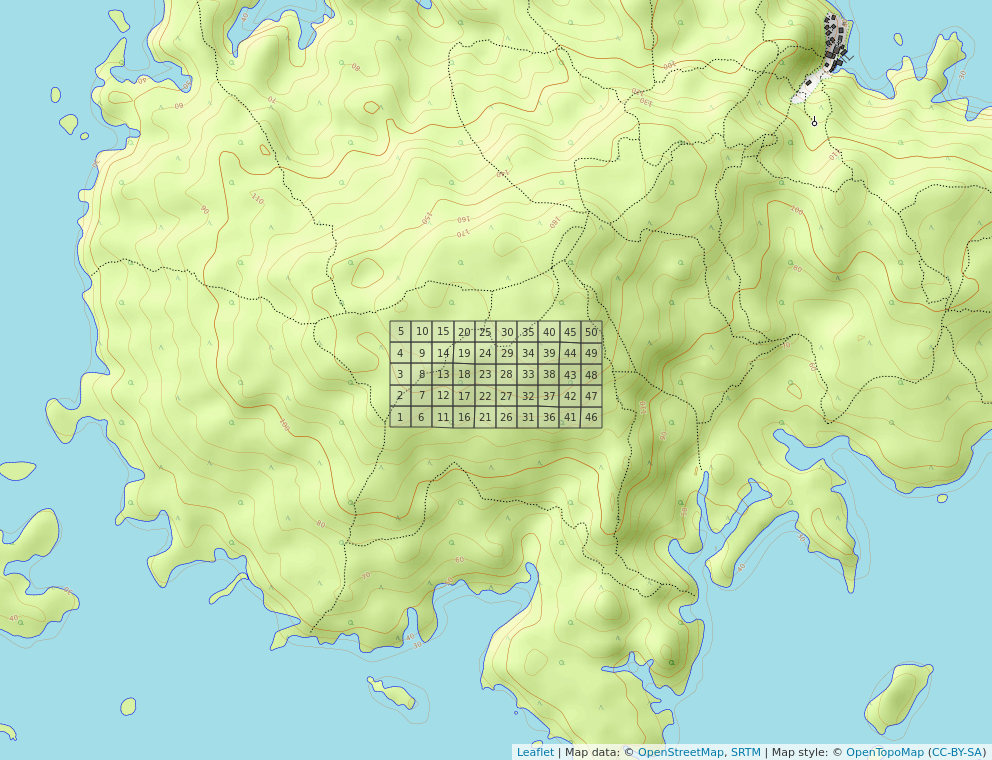
\includegraphics[width=1.00000\textwidth]{mapa_cuadros.png}
\caption{mapa de isla Barro Colorado cuadros\label{fig:bci_map}}
\end{figure}

Por igual empleo los cuadros de variables ambientales nominales y
numéricas de 1 hectárea de BCI, constituidas por categorías de edad,
habitat, geología y quebrada. Otros recursos de vital importancia son
las variables ambientales nominales de una hectárea de BCI, las
matrices, en especial de Spearman, de riqueza y abundancia de suelo, y
las de Hellinger de medición de asociación. La interacción con estas
fuentes de información ayudan a tener una aproximación más concreta
sobre la diversidad con relación a la familia tratada.

Los métodos que hasta el momento he señalado corresponden a los mapas en
los cuales aparece la parcela de 50 hectáreas en la isla Barro Colorado,
en donde se describen las variables ambientales ilustradas en matrices
que describen el comportamiento de dichas variables, y los patrones de
movilidad en el espacio que presentan las mismas, lo cual en lo adelante
permitirá comprender el mecanismo que siguen la fuerte asociación,
abundancia y riqueza de la familia en cuestión.

Todo lo anterior obedece a la parte de datos exploratorios, con
excepción de las matrices de Spearman y Hellinger que ya fueron
mencionadas y que corresponden a la sección de medición de asociación.
Está presente el segmento correpondiente a la medición de asociación, en
el que se presentan los modos Q y R, el primero referido a la medición
de asociación de sitios, en este caso por medio de la distancia, y la
similaridad de Jaccard. El modo R se refiere a la medición de la
asociación entre pares descriptores como son variables o especies,
también hago uso de la matriz de Hellinger. En el método de análisis
jerárquico, también se emplean los diagramas del árbol o dendrogramas
(método de cuerda y de Ward).

El análisis de agrupamiento, consiste en una agrupación sucesiva basada
en la repetición de un procedimiento dado de grupos de objetos, hasta
que estos encuentren su lugar, se basa en la construcción de
dendrogramas. El análsis jerárquico se caracteriza por tener un enfoque
aglomerativo, lo que implica un algoritmo ascendente, y la ordenación de
los subgrupos de objetos en un único grupo. Los algoritmos del análsis
jerárquico son los criterios de enlace, y estos a su vez se integran por
los siguientes tipos: Enlace simple, enlace completo y enlace promedio.
Los metodos de representación utilizados son: Agrupamiento aglomerativo
por enlace simple, agrupamiento aglomerativo por enlace completo, y
agrupamiento aglomerativo por enlace promedio.

También es notable la sección correspondiente a las técnicas de
ordenación y a las especies indicadoras.

La ordenación es una técnica de medición que busca determinar el grado
de asociación y de agrupamiento. Un objeto se caracteriza por sus
propiedades en un espacio n-dimensional donde cada dimensión es una
variable, un descriptor. A diferencia de la técnica de agrupamiento, o
como complemento de este, el análisis de ordenación abarca un conjunto
de técnicas que busca abarcar el tamaño ( dimensionalidad) de los datos.
El análisis de ordenación puede ser no restringido y restringido, en el
primer caso, las tendencias detectadas en el conjunto de datos suelen
estar no restringidas por otro conjunto. En el segundo caso las
tendencias detectadas en un conjunto suelen estar asociadas a otro
conjunto.

Se realiza el análisis de las especies indicadoras por medio del
estadístico de IndVal. Para el análisis de diversidad se emplean los
modos alpha y beta. Dentro de las técnicas de ordenación (restringida y
no restringida) las pruebas PCA, RDA, y CCA. Estas pruebas buscan medir
la similaridad entre los sitios con variables ambientales determinadas.
Y por último, para el análisis de ecología espacial se empleó el
correlograma con estadístico de Moran's I, que determina la existencia
de una correlación positiva o negativa.

En un correlograma, se aprecia un rectángulo cortado a la mitad de forma
horizontal, sobre este suelen alternarse barras verticales surcadas a la
mitad por un punto que representa el valor estimado (Moran's I) el cual
se lee asumiendo los valores por debajo o por encima de cero
(correlación negativa o positiva), que coincidan con dicho punto, estos
son los valores de la barra lateral izquierda. Estos puntos al franquer
la barra que representa los valores positivos y negtivos pues recrean la
autocorrelación positiva y negativa, que se expresa en sitios ubicados a
cierta cantidad de metros entre sí.

A menudo se define la biodiversidad como la variavilidad de organismos
presente en un lugar determinado, y muchos estudiosos han dejado su
impronta sobre este concepto a lo largo del tiempo. Por ejemplo, Harper
y Hawsworth, defienden que es el estudio de tres aspectos fundamentales:
Intraespecífica, interespecífica, y de ecosistemas, con los adjetivos de
genética, de organismos, y ecológica. Hubell ofrece una definición más
restringida y ajustada a la realidad actual: Biodiverisdad es sinónimo
de riqueza de especies y de abundancia relativa de especies en el
espacio en el tiempo. Magurran utiliza el término diversidad biológica y
biodiversidad como sinónimas y la define como la variedad y la
abundancia de especies en un estudio.

\section{Resultados}\label{resultados}

\subsection{Análisis Exploratorio de
Datos}\label{anuxe1lisis-exploratorio-de-datos}

A continuación muestro las mediciones de pH, mapa de pendientes, mapas
de abundancia, tanto global como de la familia, mapa de riqueza global y
de la familia, variables ambientales numéricas, y nominales en una
parcela de 50 hectáreas, integrada por subdivisiones de una hectárea,
todo ello correspondiente a la familia de las Moraceae. En el caso del
pH tenemos que es ácido, sgún los mapas y diagramas consultados, estas
condiciones para las Moraceae, y cualquier otra especie en condiciones
extremas, sería perjudicial. El pH del suelo es importante porque los
vegetales solo pueden absorver a los minerales disueltos y la variación
del pH modifica el grado de solubilidad de los minerales y nutrientes.
En el siguiente mapa, se pueden apreciar las medidas de pH presentes en
la isla de Barro Colorado en una parcela de 50 hectáreas, con un patrón
de distribución al oeste de la parcela en su variedad ácida (ver figura
\#\#2).

\begin{figure}
\centering
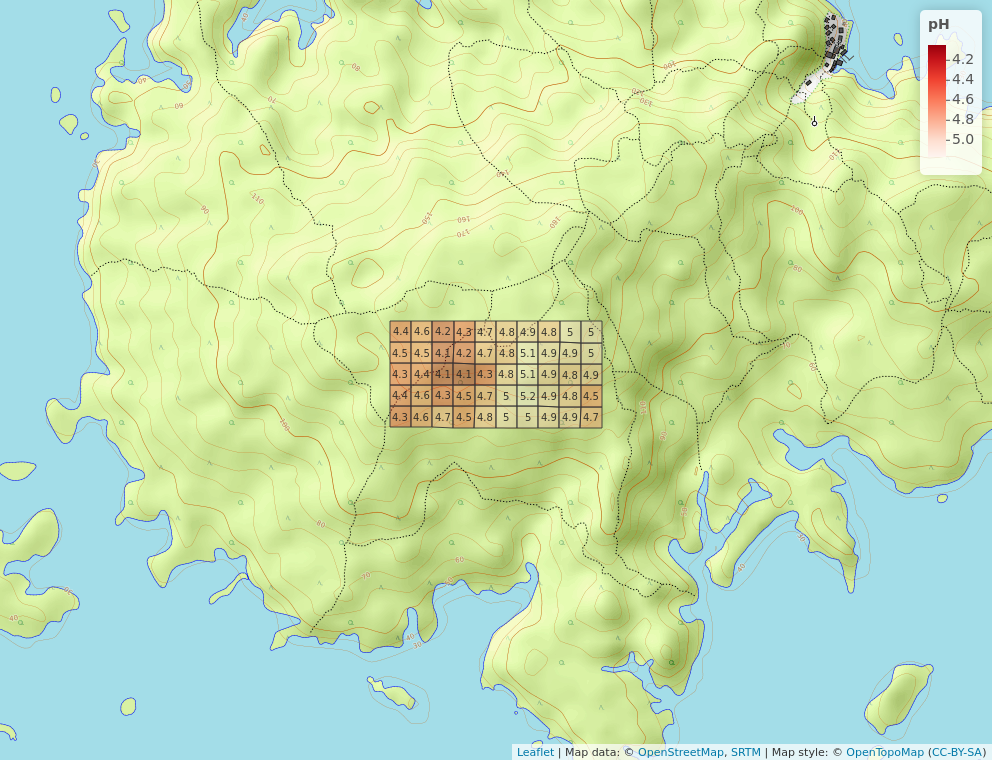
\includegraphics[width=1.00000\textwidth]{mapa_cuadros_ph.png}
\caption{mapa de la isla Barro Colorado cuadros ph\label{fig:bci_map}}
\end{figure}

Como se puede ver, el pH es eminentemente ácido, en una pacerla de 50
hectáreas, puesto que oscila en una escala de 0 a 6, con una
distribución que indica mayor concentración al oeste de dicha parcela.

En el mapa de abundacia global se advierten valores no lejanos de lo
ideal cuando se emplean parámetros de la muestra comprendidos entre 3600
y 5000, que en este caso sería una escala, en una parcela de 50
hectáreas. El Valor promedio que representaría cada hectárea en una
media hipotética sería de aproximadamente casi 4000 individuos de esta
familia, sin embargo tiende a cambiar cuando hablamos de riqueza. Si
bien existen dentro de esta familia, especies representativas de casi
todas las formas de vida leñosas, las formas más comunes entre las
especies de bibosi, son por un lado plantas hemiepífitas estranguladoras
o matapalos y por otro, plantas no epífitas con sistema propio de
sustento o higuerones (Fredericksen et al., n.d.,), (ver figura \#\#3).

\begin{figure}
\centering
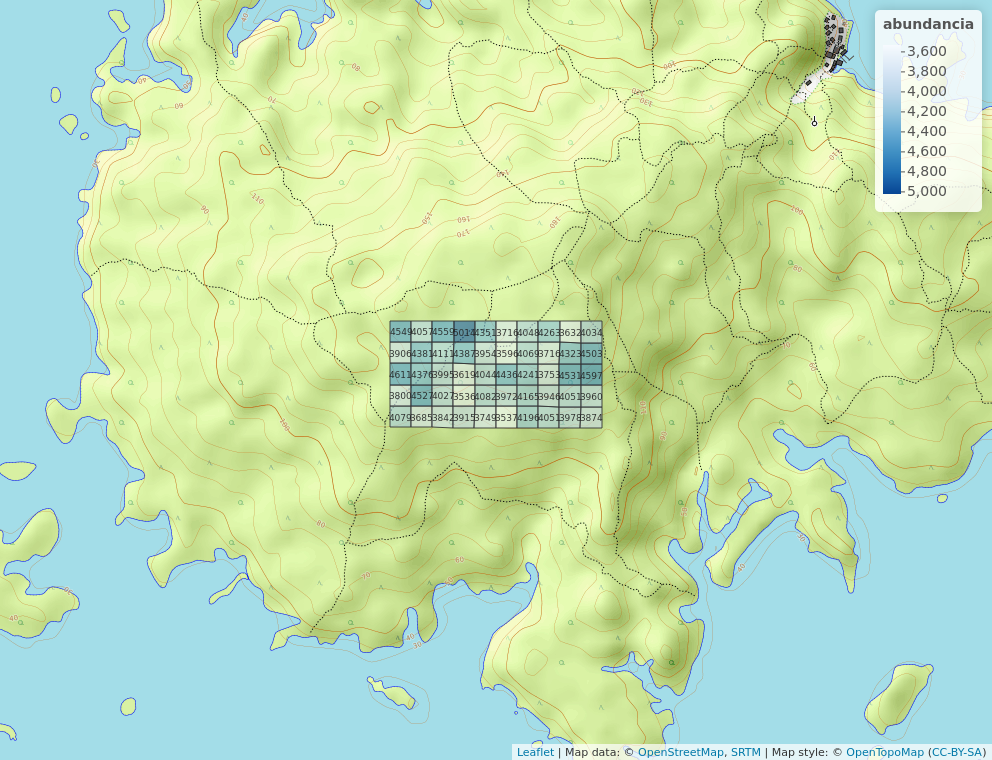
\includegraphics[width=1.00000\textwidth]{mapa_cuadros_abun_global.png}
\caption{mapa de la isla Barro Colorado abundancia global
\label{fig:bci_map}}
\end{figure}

En el mapa de abundancia de mi familia no se presenta tampoco que la
muestra por hectárea se aleja de forma marcada del parámetro empleado
para la parcela de 50 hectáreas, en este caso en un parámetro de entre
200 y 700 individuos, podría verificarse una especie de relación directa
entre el primer y segundo mapa.

En ambos casos cada hectárea adquiere valores próximos a la dimensión
numérica de individuos presentes en la parcela, para ello adjunto el
siguiente mapa sobre abundancia de mi familia (ver figura \#\#4).

\begin{figure}
\centering
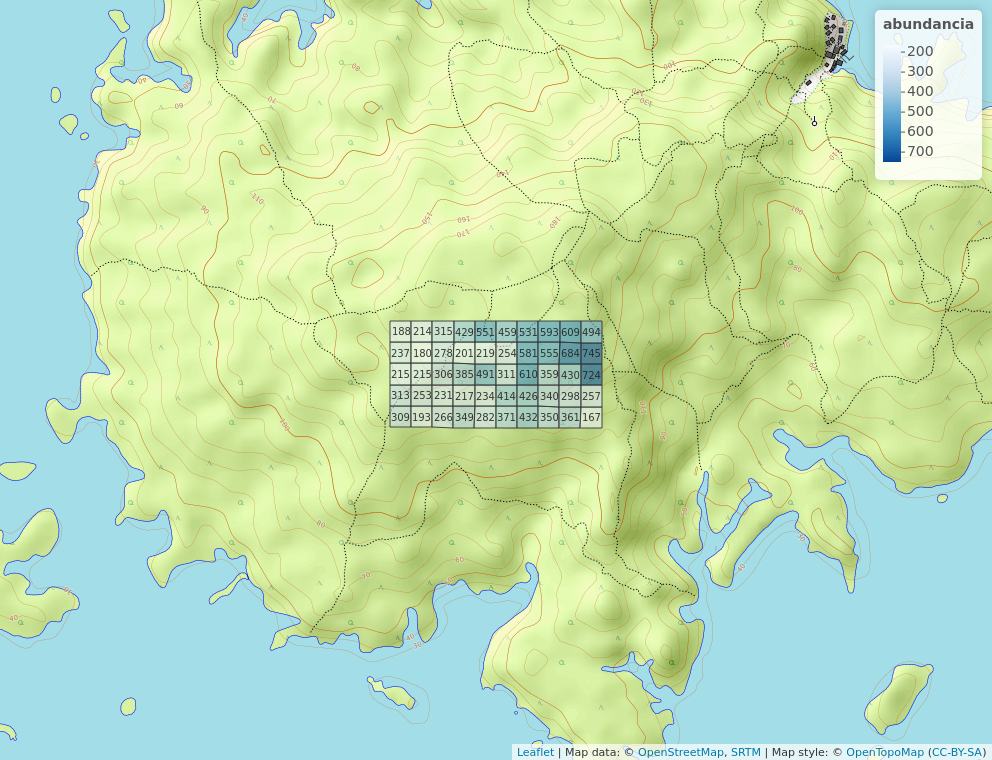
\includegraphics[width=1.00000\textwidth]{mapa_cuadros_abun_mi_familia.png}
\caption{mapa de la isla Barro Colorado abundancia de mi familia
\label{fig:bci_map}}
\end{figure}

Como puede comprobarse existen muchos individuos, en este caso citando
la abundancia, de una determinada especie de la familia de Moraceae en
una hectárea de la isla Barro Colorado, con un patrón de concentración
al noreste de la parcela, lo que muestra una amplia densidad para una
parcela de 50 hectáreas. Siendo estas plantas muchas veces ejemplares de
gran dimensión en muchos de los casos, se infiere que estas forman un
dosel impenetrable, típico de muchos bosques de la selva tropicla
centroamericana, en donde BCI no es la excepción. No solo estaríamos
hablando de Moraceae, sino de otras especies que forman la cubierta de
esta región intertropical.

La isla de Barro Colorado es realmente joven dentro de lo que es la
escala de tiempo geológico, solo tiene algo más de 100 años de
existencia lo que nos advierte de un relieve poco accidentado, debido en
gran parte a su tamaño, pero sobre todo a su edad.

En este sentido sería bueno apreciar las pendientes, y ver el valor de
la altitud en esta especie de enclave marítimo, lo que también favorece
la existencia abundante de ejemplares de Moraceae (ver figura \#\#5).

\begin{figure}
\centering
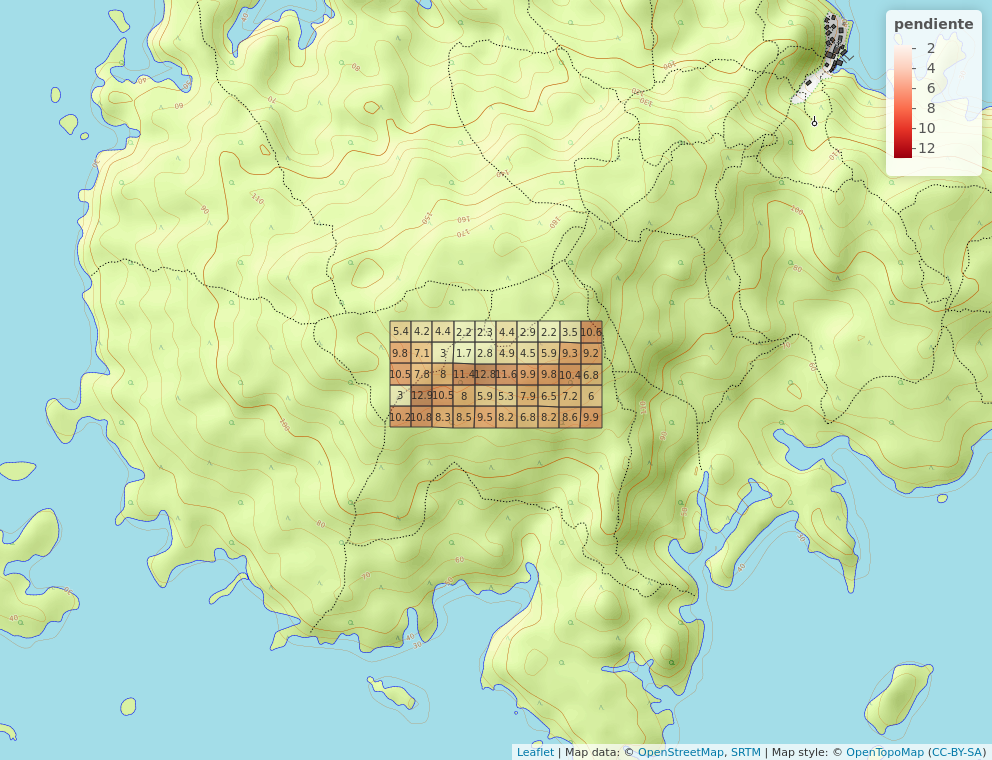
\includegraphics[width=1.00000\textwidth]{mapa_cuadros_pendiente.png}
\caption{mapa de la isla Barro Colorado cuadros y pendientes
\label{fig:bci_map}}
\end{figure}

Para una consideración general de la parcela de 50 hectáreas se destaca
gran pendiente, con un patrón de distribución al sur de la misma.

En el caso de las variables ambientales numéricas se obtiene los
siguientes valores (ver figura \#\#6)

\begin{figure}
\centering
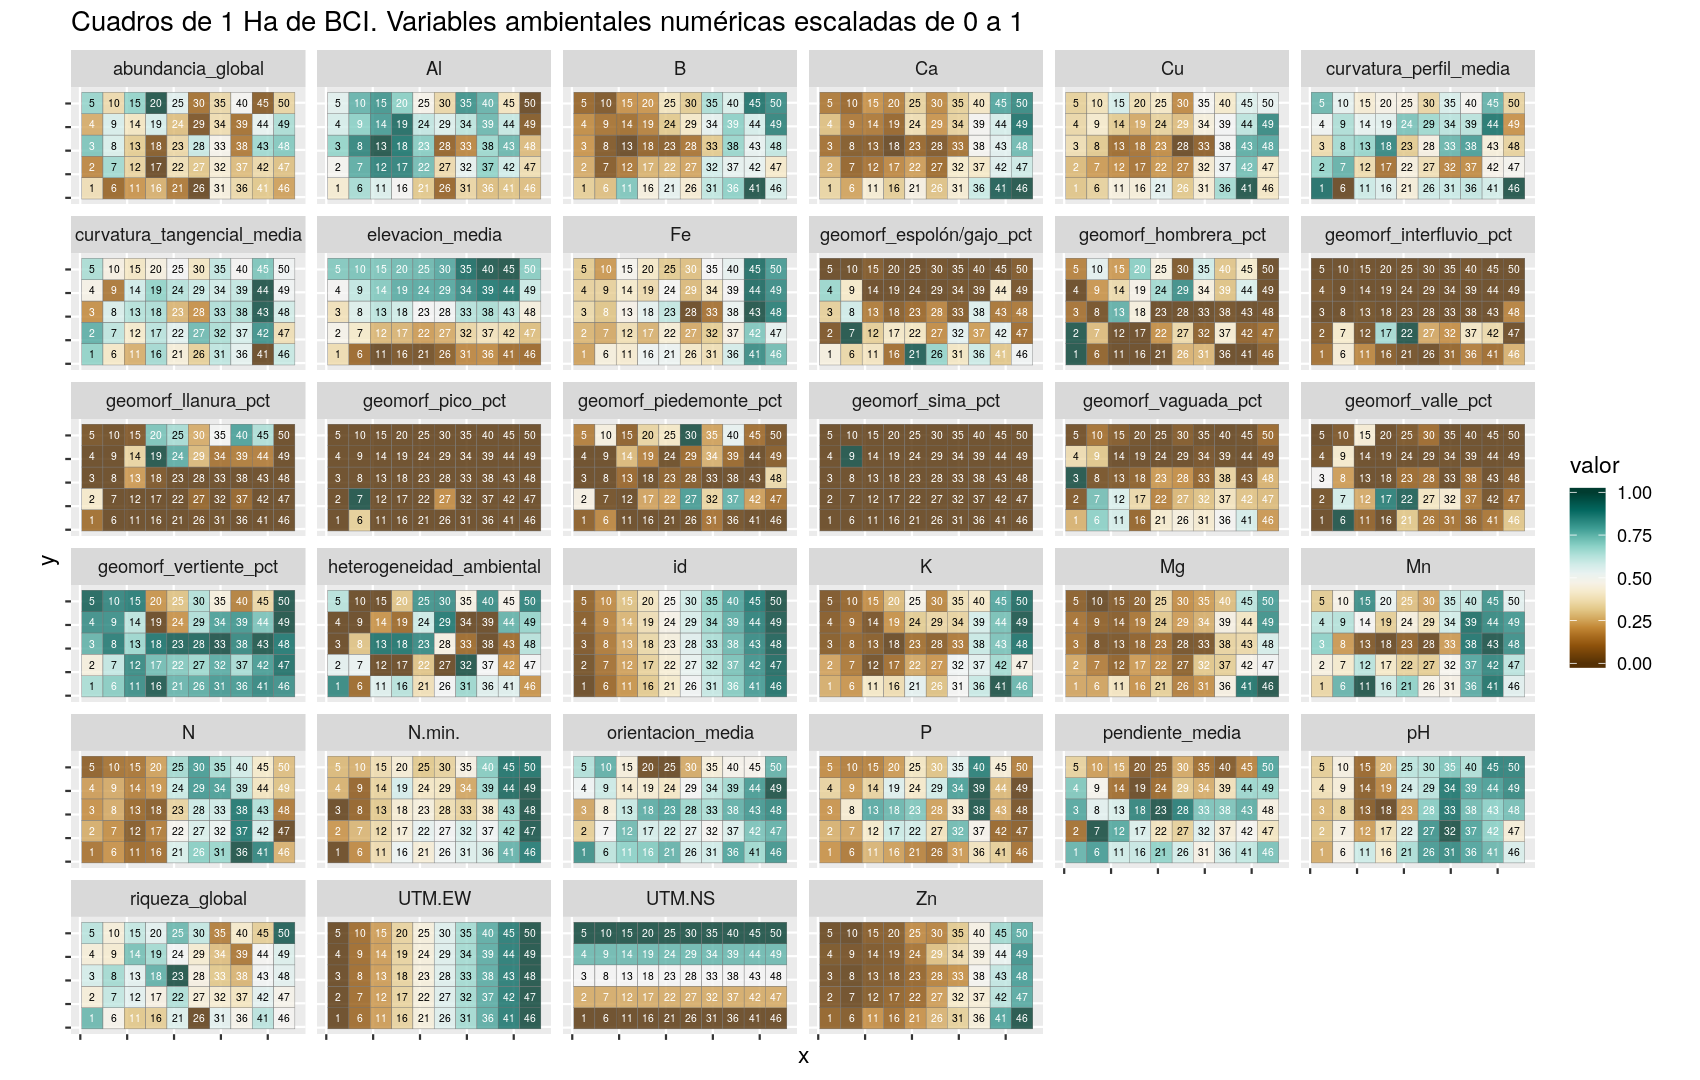
\includegraphics[width=1.00000\textwidth]{mapas_variables_ambientales_numericas.png}
\caption{mapa de la isla Barro Colorado variables ambientales numéricas
\label{fig:bci_map}}
\end{figure}

Aquí podemos ver una especie de síntesis de las informaciones que
ofrecen las variables ambientales de una hectárea, escaladas de 0 a 1.
En el caso de las geoformas, correspondientes a llanuras, se obtienen
valores grandes en un segmento de la escala que va de 0.00 a 0.25, lo
que refleja un terreno eminentemente llano. Con relación a las vrtientes
ocurre todo lo contrario, se obtienen valores grandes, en el segmento de
la escala que va de 0.75 a 1.00, lo que se refiere a mayor inclinación
en contraste con las tierras llanas. Otra geoforma como es el caso de
los valles, presenta valores muy pronunciados en los segmentos bajos de
la escala citada. Los valores de la escala muestran amplias diferencias
entre unas variables y otras, pero dentro de la misma escala, suele
verse la superioridad de una sobre otra.

En el mapa de variables ambientales nominales, se aprecia la dinámica de
algunas variables ambientales (ver figura \#\#7)

\begin{figure}
\centering
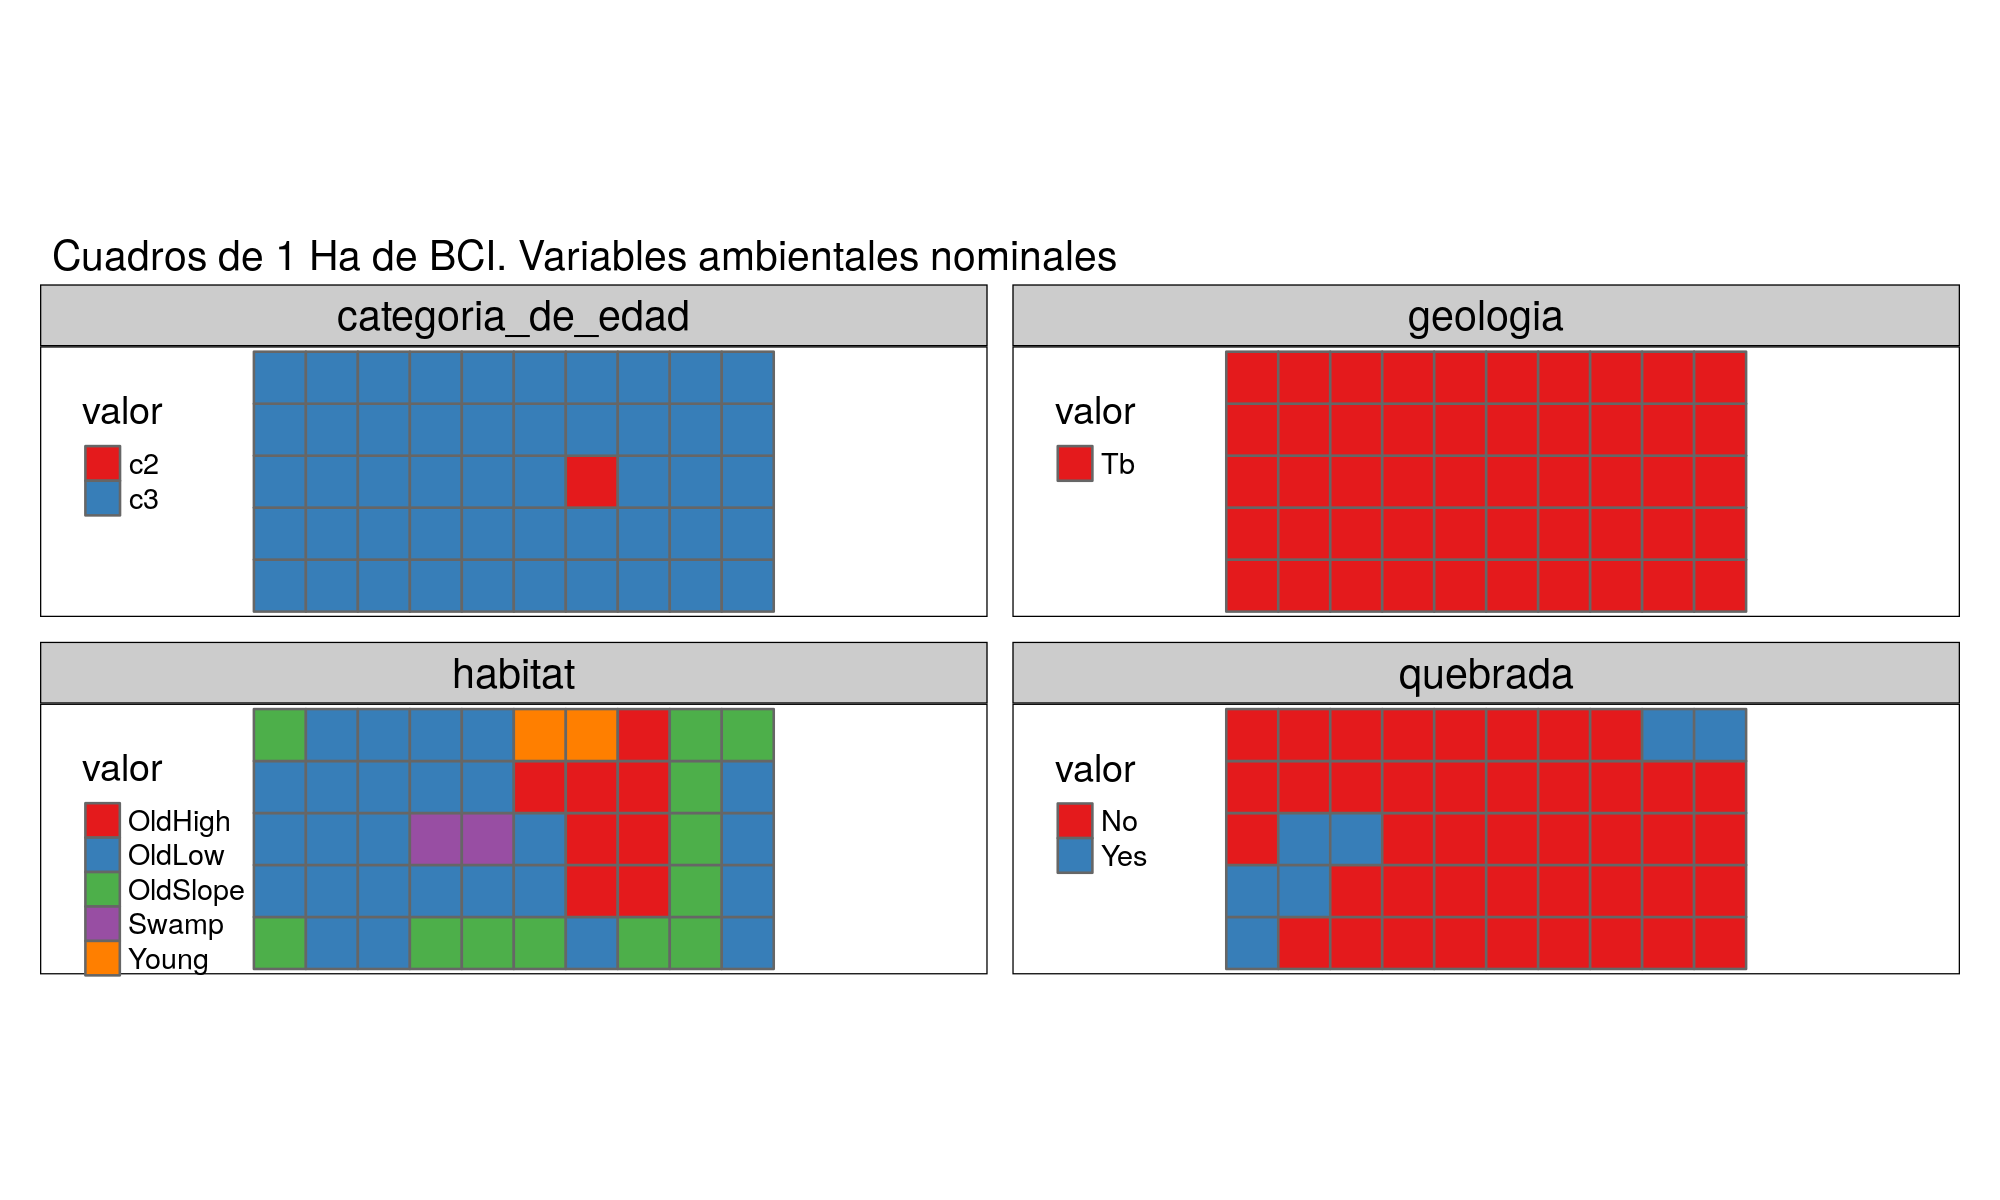
\includegraphics[width=1.00000\textwidth]{mapas_variables_ambientales_nominales_tmap.png}
\caption{mapa de la isla Barro Colorado variables ambientales nominales
\label{fig:bci_map}}
\end{figure}

En esta matriz se distinguen variables como la categoría de edad,
geología de la región, hábitat, y la quebrada. El hábitat de bosque
viejo en terreno alto (OldHigh), se destaca por su relativa minoría. En
tanto que el bosque viejo en relieve bajo (OldLow) es el más abundante.
El bosque viejo con pendiente (OldSlope), es relativamente abundante. El
pantano es escaso (Swamp), así también el bosque joven (Young). En
cuanto a la geología tenemos que el tipo de roca predominante es de tipo
intrusivo o plutónica. Las quebradas o barrancos son estrechos. Existen
dos grandes categorías dentro de la variable de edad, el bosque viejo en
terreno bajo, y el bosque viejo en terreno alto. De lo anterior se
infiere que existe más terreno bajo con bosque viejo en BCI en una base
gelógica joven, que con las demás variables.

El mapa de riqueza presenta un formato similar a los de abundancia, con
comportamientos diferenciados por hectárea, comparados con la parcela de
50 hectáreas. En el siguiente mapa puede apreciarse la riqueza de la
famiia botánica bajo estudio (Moraceae) por hectárea (ver figura \#\#8).

\begin{figure}
\centering
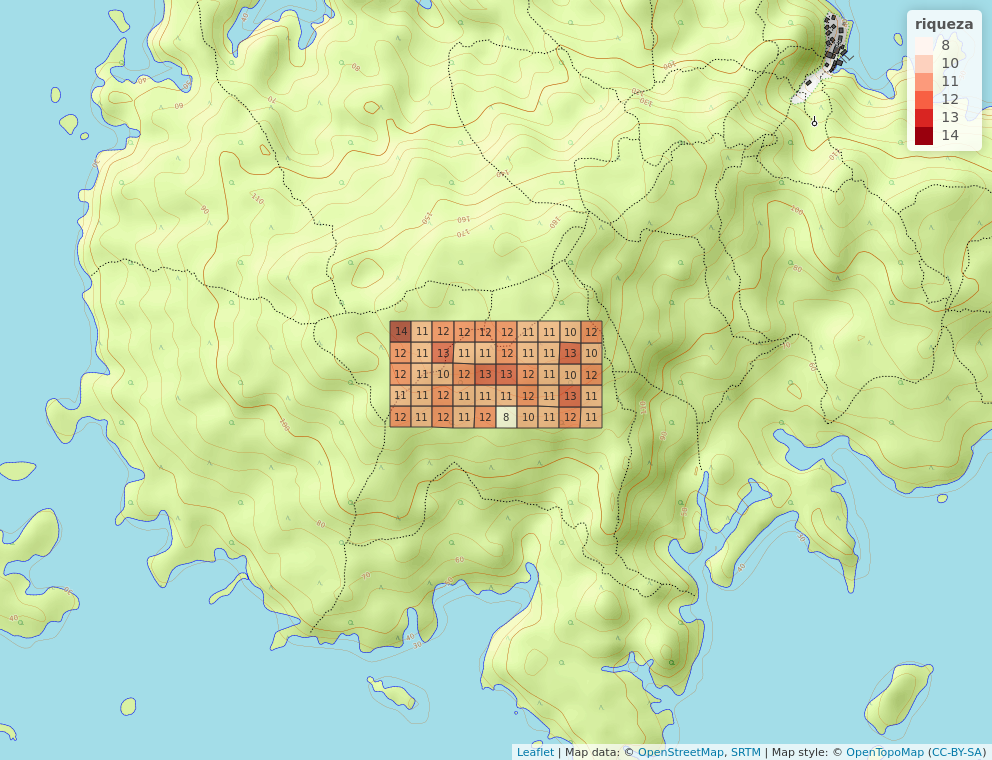
\includegraphics[width=1.00000\textwidth]{mapa_cuadros_riq_mi_familia.png}
\caption{mapa de la isla Barro Colorado cuadro de riqueza mi familia
\label{fig:bci_map}}
\end{figure}

En esta parte puede apreciarse que la riqueza es casi la misma por
hectárea, acercándose al nivel superior de la escala, así se puede
asumir que el grado de dispersión de algunos individuos de la familia
Moraceae es casi nulo. Existe una gran riqueza de estas plantas que
ayudan en gran parte a mantener este grandioso ecosistema.

Ya para el mapa de riqueza global se advierten mayores contrastes por
hectárea, pero igual se impone la diversidad, la multiplicidad de
individuos es asombrosa (ver figura \#\#9). La riqueza global presenta
un patrón de distribución noroeste-sureste.

\begin{figure}
\centering
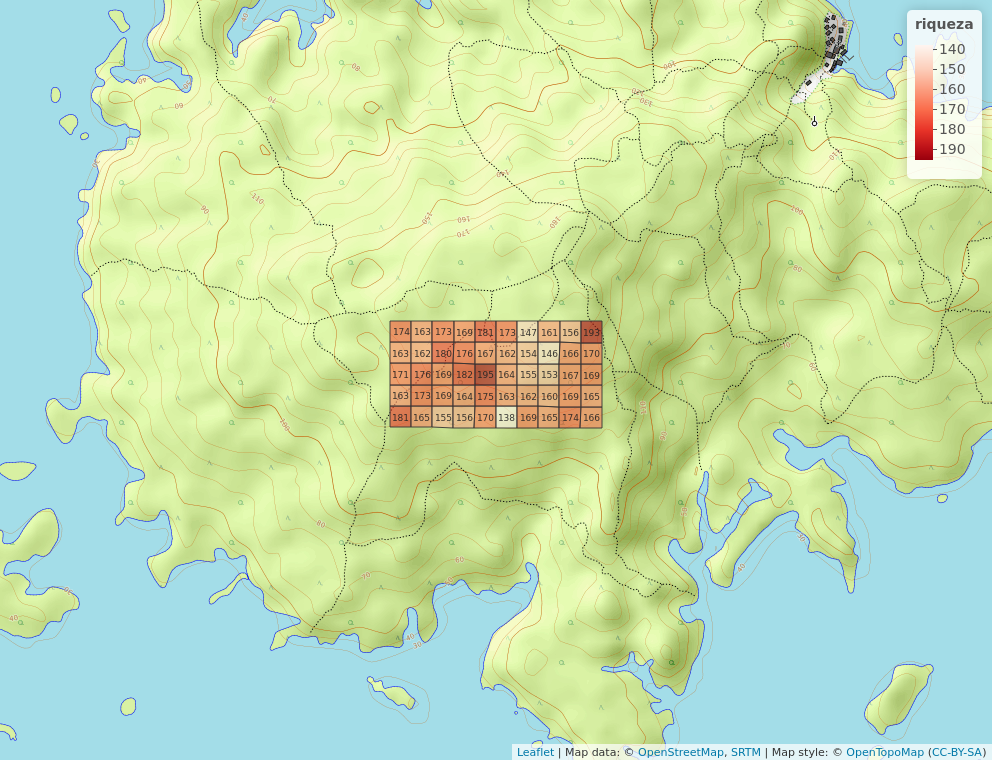
\includegraphics[width=1.00000\textwidth]{mapa_cuadros_riq_global.png}
\caption{mapa de la isla Barro Colorado riqueza global
\label{fig:bci_map}}
\end{figure}

En los cuadros de variables ambientales, se registran las diferencias
entre unas y otras, se distinguen tierras bajas de otras no muy altas.
Pero no solo se analizan los rasgos geomorfológicos, otras variables
ofrecen tambien allí su concurso. Aprecen valores de pH, riqueza global
por igual, abundancia global, entre otras variables.

\subsection{Medición de Asociación (Modos Q y
R)}\label{mediciuxf3n-de-asociaciuxf3n-modos-q-y-r}

En esta parte se aborda lo que es la medición de asociación, tomando en
cuenta lo que son los valores de disimilaridad o distancia, así como las
matríces de correlación. Dentro de los modelos de medición de asociación
existen los modos Q y R, en este caso de la distancia o disimilaridad,
tenemos el modo Q que describe la distancia entre objetos cuantitativos.
La paradoja de Orlóci plantea que la distancia euclidea es más pequeña
entre sitios que no comparten especies que entre sitios que sí las
comparten. A continuación se presenta una matríz de disimilaridad (ver
figura \#\#10).

\begin{figure}
\centering
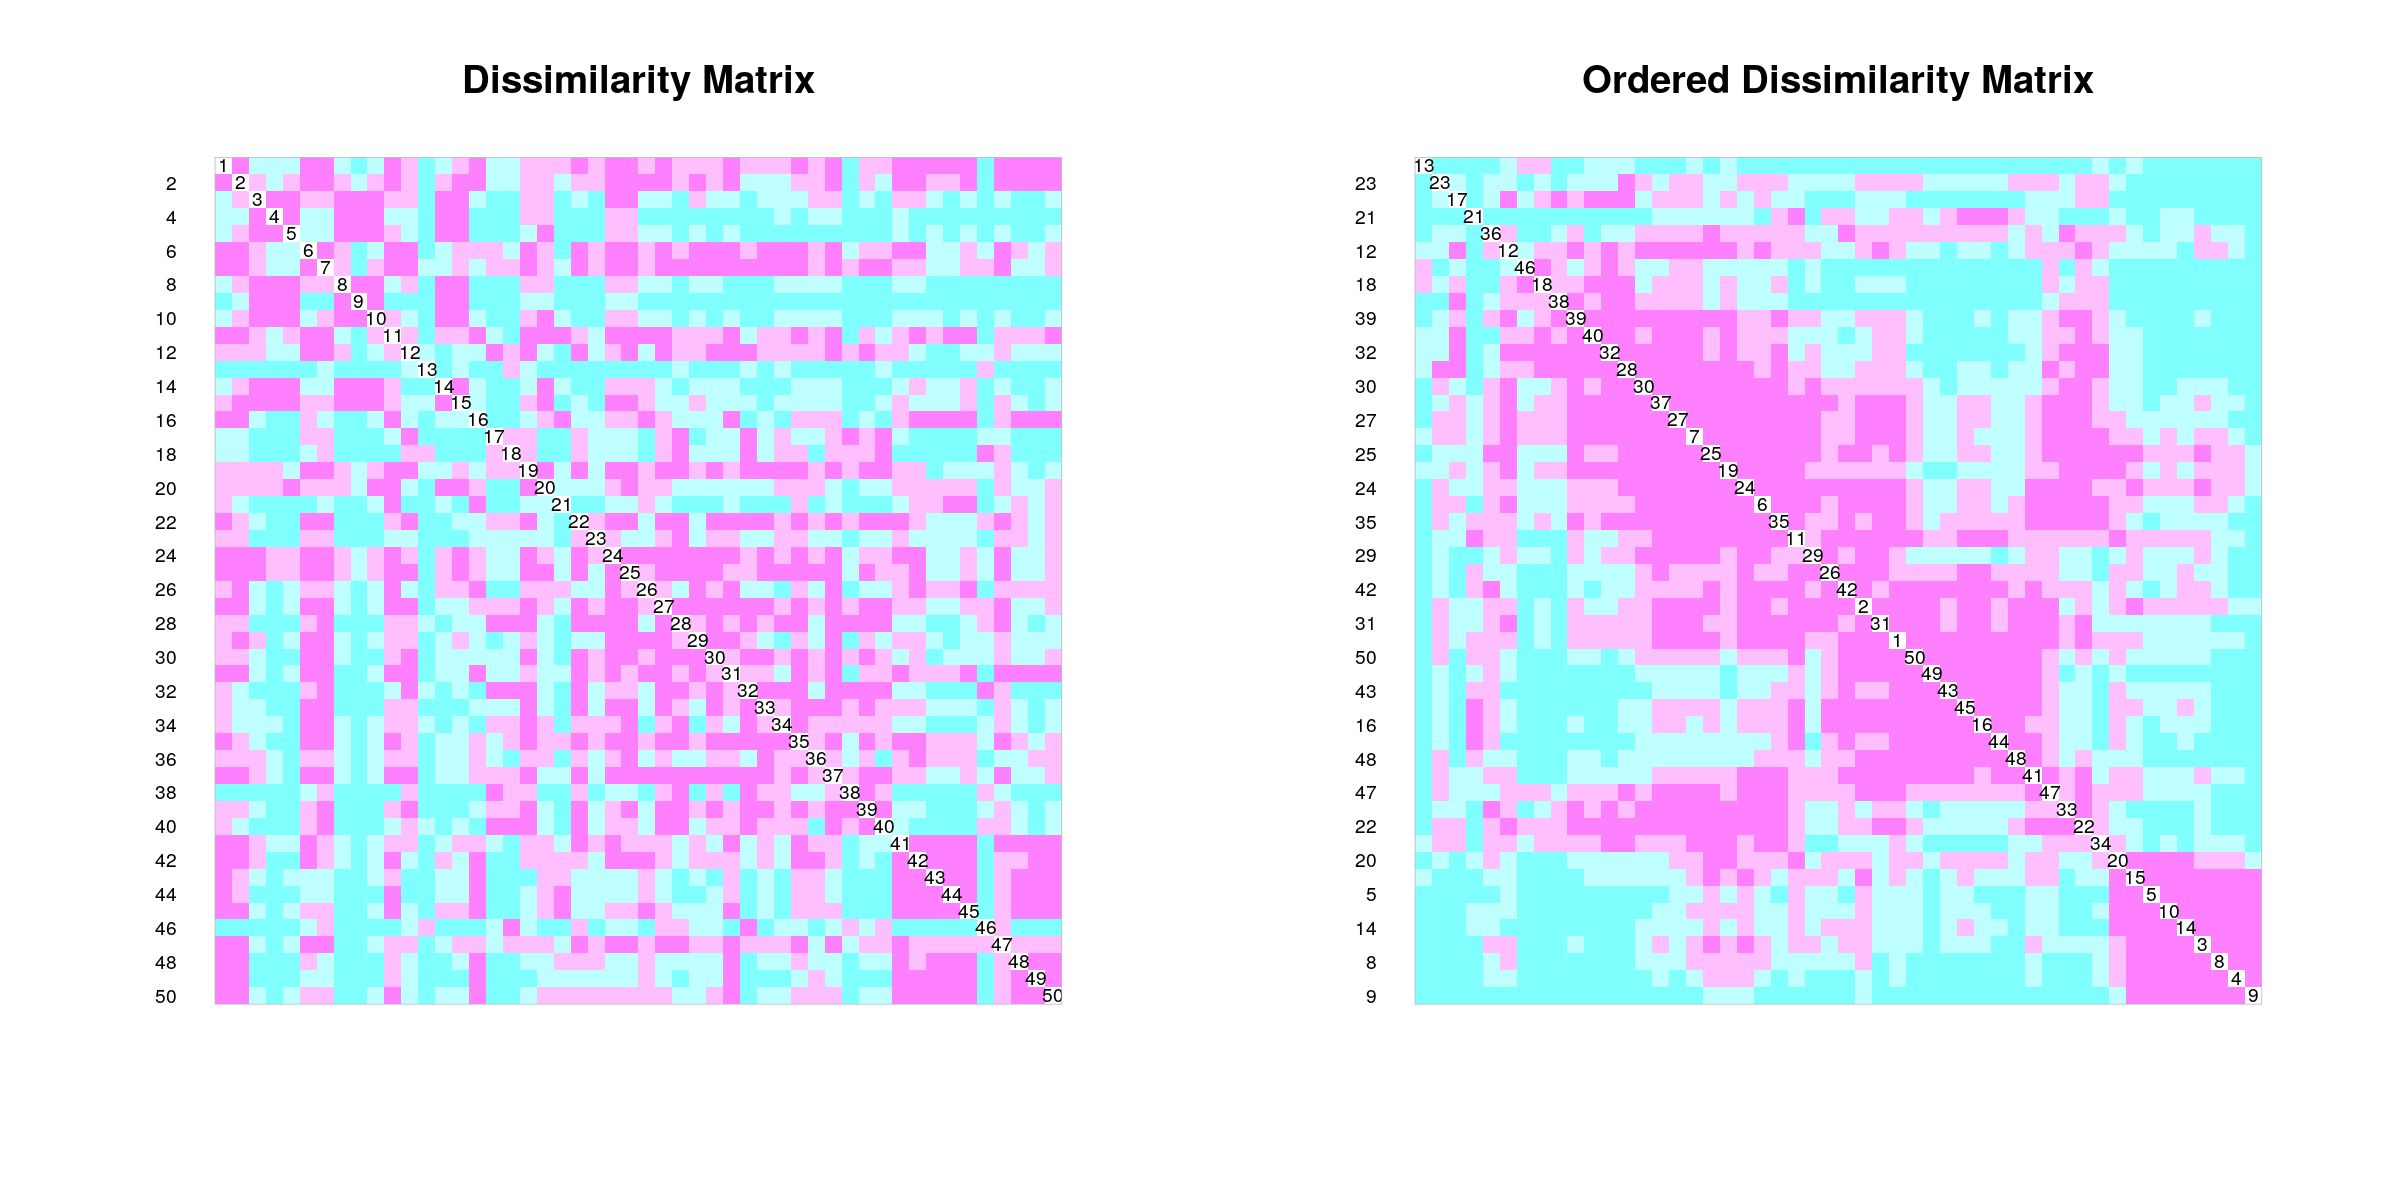
\includegraphics[width=1.00000\textwidth]{matriz_disimilaridad_hellinger.png}
\caption{mapa de la isla Barro Colorado matriz disimilaridad hellinger
\label{fig:bci_map}}
\end{figure}

La matrz de disimilaridad es una representación de la medición de
asociación entre objetos en el modo Q, como serían los sitios de
muestreo. En esta matriz se puede apreciar una fuerte asociación entre
objetos y esto lo indica la continuidad del color rosado (cuadro de la
derecha). En este caso nos referimos a la matriz de la derecha, que es
la matriz ordenada, a partir de la primera. Por ejemplo entre los sitios
40 y 35 existe una distancia muy pequeña entre sitios parecidos para la
matriz ordenada. La transformación Hellinger permite hacer la
interpretación en base a dos colores representativos: Color fucsia
(magneta, rosa) que equivale a corta distancia, muy similar, y el cian o
celeste que significa gran distancia o poco similar, todo esto con
relación a los elementos de la familia de las moraceae. Algunos de los
valores de disimilaridad o de distancia entre objetos que podemos
apreciar dentro de la transformación Hellinger son los siguientes: Entre
los sitios 2 y 1, tenemos que la distancia (dbl) es de 0.187, entre 3 y
1 es de 0.439, entre 4 y 1 es de 0.499, entre 5 y 1 es de 0.430, entre 6
y 1 de 0.297, entre 7 y 1 es de 0.280, entre 8 y 1 es de 0.492, entre 9
y 1 es de 0.584, entre 10 y 1 es de 0.425, y entre 11 y 1 es de 0.269 lo
que revela una escasa distancia o disimilaridad entre los objetos.

A continuación presento una versión mejorada de la matríz ordenada de
datos cuantitativos de especies (abundancia) con fuerte asociación en la
diagonal (ver figura \#\#11).

\begin{figure}
\centering
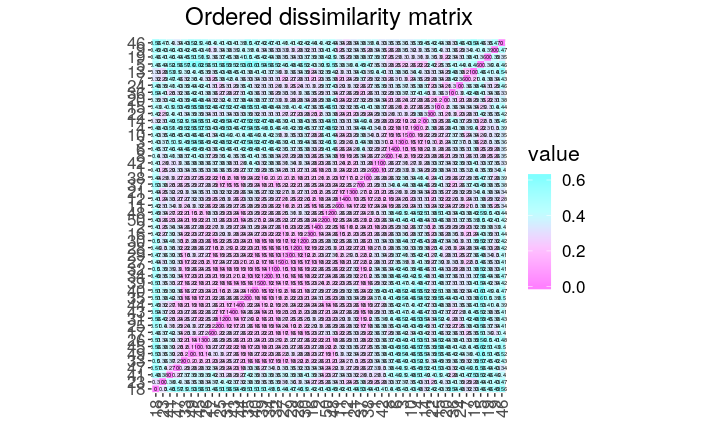
\includegraphics[width=1.00000\textwidth]{matrizdedisimilaridad.png}
\caption{mapa de la isla Barro Colorado matriz disimilaridad
\label{fig:bci_map}}
\end{figure}

En esta matriz de disimilaridad o de distancia vienen a recrearse los
anteriores casos de abundancia de los mapas de la Isla de Barro
Colorado. En la diagonal se pueden apreciar los sitios que poseen
características similares con la menor distancia(color rosado), mientras
que en los demás lugares se aprecian lugares con características
similares a mayor distancia y con una menor asociación (color cian o
celeste). Hasta el momento me he centrado en el modo Q que mide el nivel
de asociación por medio de la disimilaridad o similiridad. Algo
sumamente importante dentro del modo Q, en este caso basándome en datos
binarios (presencia/ausencia) es la famosa distancia de Jaccard, la
misma se puede expresar como la proporción de especies no compartidas.
Para el caso correspondinte de los datos de moraceae, la distancia (dbl)
muestra los siguientes resultados para algunos sitios: Entre 2 y 1, la
distancia es de 0.22, para 3 y 1 es de 0.33, entre 4 y 1 es de 0.222,
para 5 y 1 es de 0.3, para 6 y 1 es de 0.333, para 7 y 1 es de 0.222,
para 8 y 1 es de 0.333, para 9 y 1 es de 0.333, para 10 y 1 es de 0.4, y
para 11 y 1 es de 0.333, evidenciando en este caso una fuerte
asociación.

La similaridad es la proporción de objetos compartiods entre sitios, en
la siguiente gráfica de la matriz pueden apreciarse las espcecies
compartidas entre sitios (ver figura \#\#12).

\begin{figure}
\centering
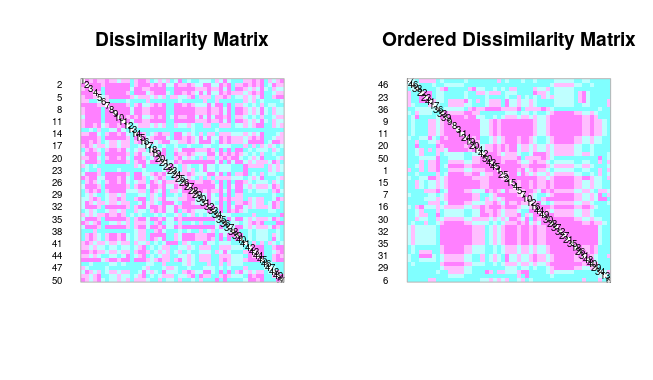
\includegraphics[width=1.00000\textwidth]{matriz_similaridad.png}
\caption{mapa de la isla Barro Colorado matriz disimilaridad
\label{fig:bci_map}}
\end{figure}

Pueden notarse en los bloques de colores las especies compartidas entre
sitios, y que son exclusivas de dichos sitios. Por ejemplo para las
variables a, b y c, que se desprenden de la fómula, incluida en los
scripts reproducibles que sirven de soporte a este trabajo, de la
similaridad, donde a representa el número de especies compartidas, b es
el número de especies exclusivas del sitio 2 y c el numero de especies
exclusivas del sitio 1. La cantidad de especies compartidas entre sitios
con relación a las moraceae es grande, esto debido a la ausencia de
ceros, hecho que en la paradoja de Orlóci refleja cercanía según la
distancia euclídea que hace ver próximos los lugares o sitios que no
comparten especies o individuos.

En el modo R se mide la asociación entre pares descriptores, es decir
variables o especies, mediante la covarianza y la correlación. Por
ejemplo para las variables a, b y c, que se desprenden de la fómula de
la similaridad, donde a representa el número de especies compartidas, b
es el número de especies exclusivas del sitio 2 y c el numero de
especies exclusivas del sitio 1.

Un ejemplo ilustrativo sería el mapa de calor (ver figura \#\#13)

\begin{figure}
\centering
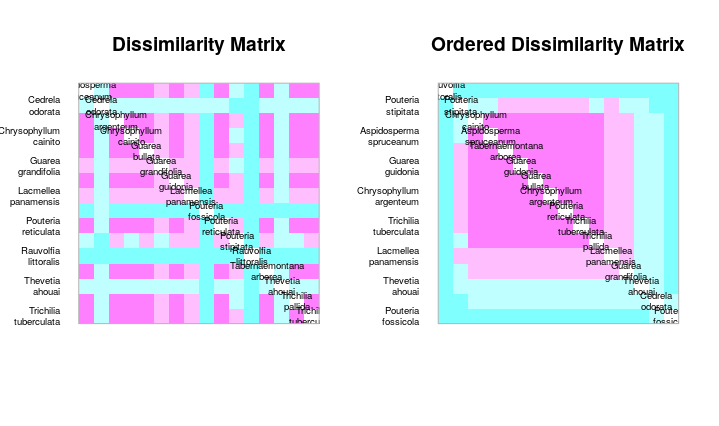
\includegraphics[width=1.00000\textwidth]{mapadecalor.png}
\caption{mapa de la isla Barro Colorado mapa de calor
\label{fig:bci_map}}
\end{figure}

En el mapa de calor mostrado se percibe una relación de dependencia en
la diagonal de la derecha, esto es lo que se mide en el modo R, la
asociación entre elementos descriptores, en este caso la abundancia de
especies como variables. Entre la \emph{Cainito aspidosperma} y la
\emph{trichinia tuberculata} se nota una fuerte dependencia, evidenciado
por la continuidad del color fucsia o rosa. Lo mismo no ocurre con los
colores de los bordes que reflejan franjas más pequeñas, y a su vez
degradadas, lo que evidencia ausencia de dependencia. Esto así cuando se
trata del modo R aplicado a datos cuantitativos de especies, que
reflejan la abundancia, al igual que el modo Q, el Modo R se aplica para
datos binarios, así tambien para la abundancia de variables
(coeficientes de spearman y pearson).

A continuación muestro una matriz de abundancia y riqueza de suelo según
el coeficiente de Spearman, con valores que aumentan y disminuyen de
este a oeste, y de norte a sur, los valores en rojo presentan los
valores más altos, y los azules los más bajos (ver figura \#\#14).

\begin{figure}
\centering
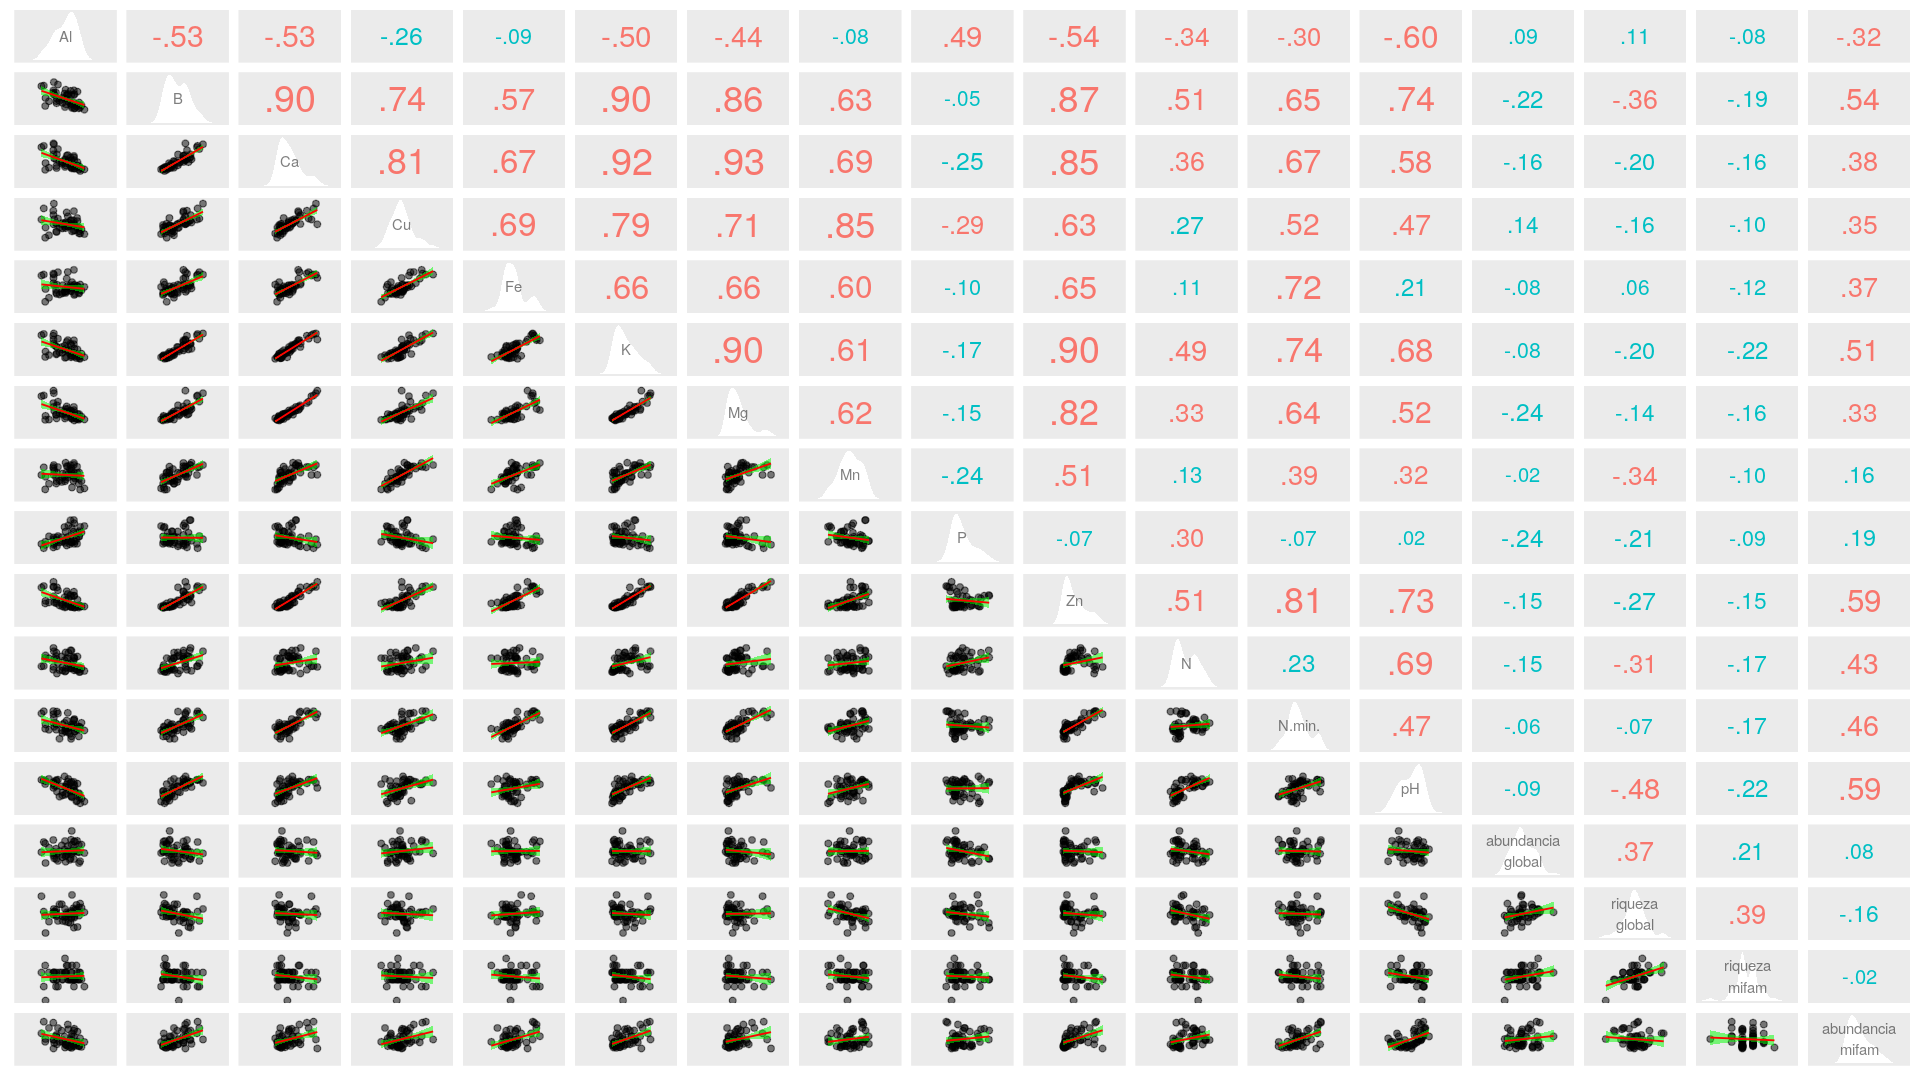
\includegraphics[width=1.00000\textwidth]{matriz_correlacion_suelo_abun_riq_spearman.png}
\caption{mapa de la isla Barro Colorado abundancia y riqueza de suelo
\label{fig:bci_map}}
\end{figure}

En la medición de asociación en los modos antes mencionados, se obtiene
una apreciación estadística de la distribución de sitios, especies y
variables ambientales presentes en la isla Barro Colorado que reflejan
la cuatificación de las comunidades de moraceas presentes en dicha isla,
así como la mayor o menor concentración de las mismas con relación al
grado de asociación presente en los sitios.

\subsection{Agrupamiento Jerárquico}\label{agrupamiento-jeruxe1rquico}

A continuación se muestran los resultados de esta sección
correspondiente a la familia de Moraceae.

\subsubsection{Agrupamiento Aglomerativo por Enlace
Simple}\label{agrupamiento-aglomerativo-por-enlace-simple}

\begin{figure}
\centering
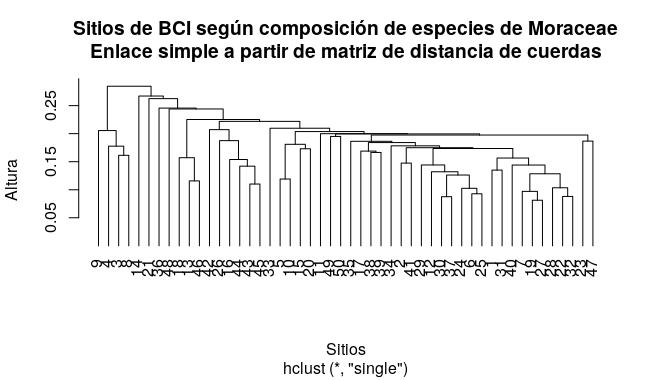
\includegraphics[width=1.00000\textwidth]{sitios_composicion_distancia_cuerdas.png}
\caption{mapa de la isla Barro Colorado sitios de composición por
distancia de cuerda \label{fig:bci_map}}
\end{figure}

Cuando se construye este dendrograma, empleando la menor distancia entre
sitios, se obtiene una matriz de cuerdas o matriz normalizada (ver
figura \#\#15). En este dendrograma se puede apreciar que en la parcela
de 50 hectáreas aún cuando se construyeran subgrupos cada vez más
pequeños para la familia de Moraceae, se formaría una innumerable
cantidad de los mismos, lo que pone sobre relieve la gran similaridad
entre sitios que albergan a especies de dicha familia, ya sea en función
de la abundancia o de la riqueza. Este dendrograma recuerda la forma de
una escalera (ver figura \#\#15).

\subsubsection{Agrupamiento Aglomerativo por Enlace
Completo}\label{agrupamiento-aglomerativo-por-enlace-completo}

\begin{figure}
\centering
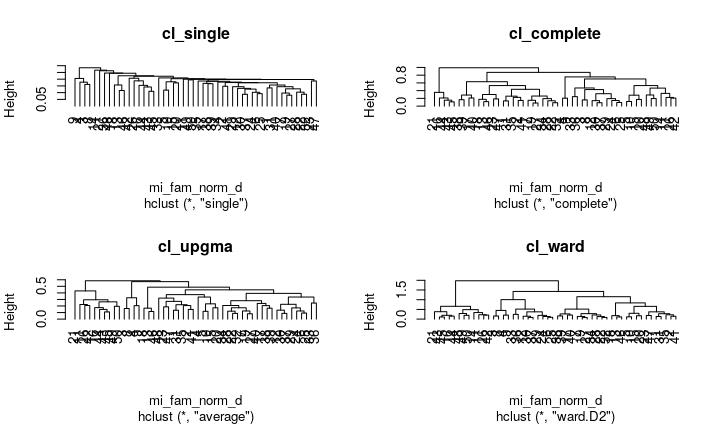
\includegraphics[width=1.00000\textwidth]{analisis_interpretacion_dendrogramas.png}
\caption{mapa de la isla Barro Colorado analisis interpretación
dendrogramas \label{fig:bci_map}}
\end{figure}

En esta imagen, aunque se ilustran los tipos considerados de
dendrogramas (ver figura \#\#16), nos interesa el completo. En el
agrupamiento aglomerativo por enlace completo, el criterio empleado es
la mayor distancia o menor similaridad, el vecino más lejano. En este
dendrograma se muestra una escalera pero con menor sucesión, se
distinguen grupos de dendrogramas como en el caso anterior, solo que en
esta ocasión los grupos con mayor distancia son poco numerosos en
contraste con los los grupos que presentan la menor distancia, y la
altura dominante para los cuadros mayores es de 0.8 en su generalidad.

\subsubsection{Agrupamiento Aglomerativo por Enlace
Promedio}\label{agrupamiento-aglomerativo-por-enlace-promedio}

\begin{figure}
\centering
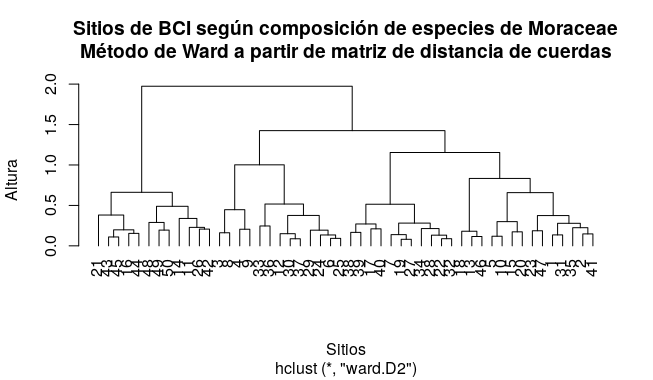
\includegraphics[width=1.00000\textwidth]{sitios_metodo_ward.png}
\caption{mapa de la isla Barro Colorado sitios de composición por
distancia de cuerda \label{fig:bci_map}}
\end{figure}

El método de Ward, aunque no es un método por enlace (ver figura
\#\#17), lo elijo por su fácil comprensión (en este caso sería el UPGMA,
para el caso de la media o promedio), recuerda la silueta de una
pirámide toscamente dibujada, con una interpretación visual más factible
que en los casos anteriores. Existe una regularidad en los subgrupos, lo
que refleja, al igual que en las secciones anteriores una fuerte
asociación, mayor similaridad que disimilaridad en las partes dominantes
o más visibles. Un ejemplo de visualización lo ofrece el modelo de
agrupación aglomerativa por enlace promedio, UPGMA, en el cual aparecen
siluetas aglomerativas y repetitivas que reflejan una continuidad en la
similaridad de los subgrupos.

\subsubsection{Interpretación de Agrupamiento
Jerárquico}\label{interpretaciuxf3n-de-agrupamiento-jeruxe1rquico}

En esta parte estamos a la altura de elegir métodos que nos permitan
minimizar la mayor cantidad posible de unidades de grupos en los
dendrogramas. Se establece la correlación cofenética y para la misma los
métodos convenientes son los de Ward y el UPGMA. En esencia consiste en
obtener la menor cantidad posible de siluetas que se distinguen por la
existencia de pequeños grupos de figuras. En la siguiente imagen pueden
apreciarse los cortes de las siluetas en tamaños menos complicados de
analizar y no muy distantes en su dimensión, por lo menos en los dos
primeros cuadros (ver figura \#\#18).

\begin{figure}
\centering
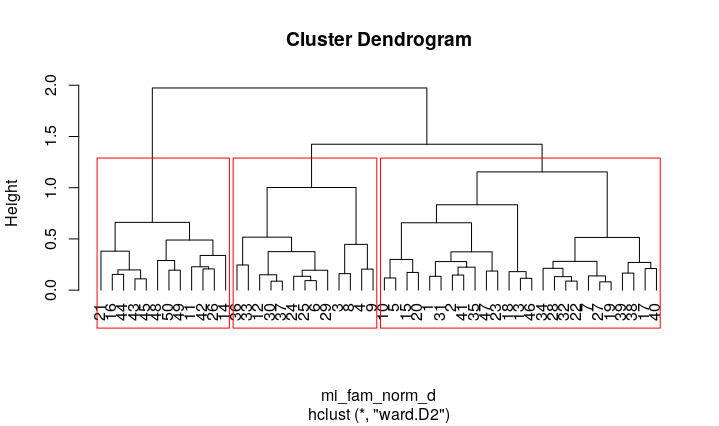
\includegraphics[width=1.00000\textwidth]{agrupamiento_dendrograma.png}
\caption{mapa de la isla Barro Colorado sitios de composición por
distancia de cuerda \label{fig:bci_map}}
\end{figure}

El método Ward es uno de los más ideales para elegir un dendrograma
único que permita apreciar por simple inspección el tamaño de las
siluetas, y el número de sitios que contienen, en este caso serían tres
cuadros de 12 y 13 sitios para el primer y segundo cuadro
respectivamente, y de 25 sitios para el tercero, todos a una altura de
1.3 aproximadamente dentro del dendrograma. En este dendrograma pueden
apreciarse las siluestas más fácilmente que en los ejemplos anteriores.

Una forma de ilustrar mejor la disimilaridad y la similaridad entre los
agrupamientos o dendrogramas es por medio del mapa de calor de la matriz
de comunidad fusionado con el dendrogrma. En eta ilustración se
distinguen los sitios que presentan mayor grado de asociación. Puede
verse que el dendrograma está cortado a la mitad, y los sitios que
presentan mayor similaridad o menor distancia están al centro y en los
extremos, por ejemplo, los grupos 13 y 18 presentan una fuerte
asociación, y en general los grupos dispuestos de forma vertical
presentan mayor similaridad que los dispuestos de forma horizontal (ver
figura \#\#19).

\begin{figure}
\centering
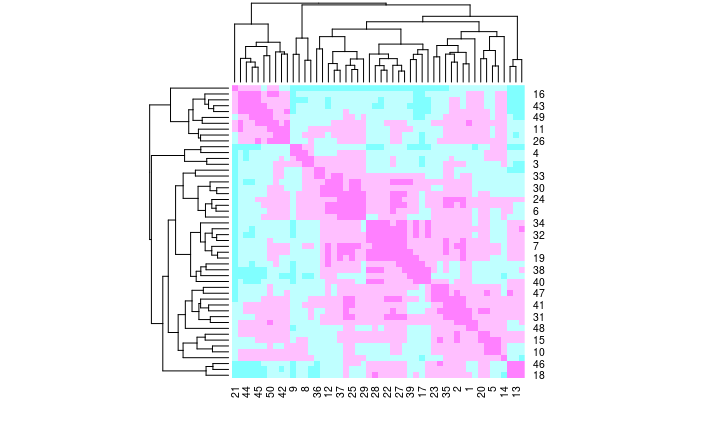
\includegraphics[width=1.00000\textwidth]{comparacion_dendrograma_mapa_calor.png}
\caption{mapa de la isla Barro Colorado sitios de composición por
distancia de cuerda \label{fig:bci_map}}
\end{figure}

\begin{figure}
\centering
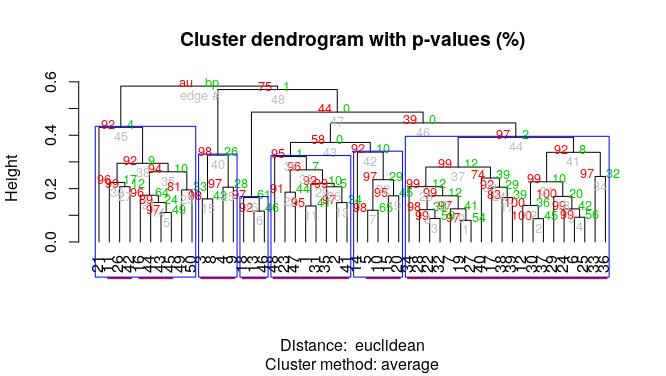
\includegraphics[width=1.00000\textwidth]{multiescalar_bootstrap.png}
\caption{mapa de la isla Barro Colorado remuestreo multiescalar por
Bootstrap \label{fig:bci_map}}
\end{figure}

En el mapa anterior pueden verse las probabilidades, y la anchura de las
siluetas de los cuadros que contienen los subgrupos con mayor
similaridad, lo que refleja los posibles cortes que se podrían hacer
sobre el dendrograma (ver figura \#\#20).

\begin{figure}
\centering
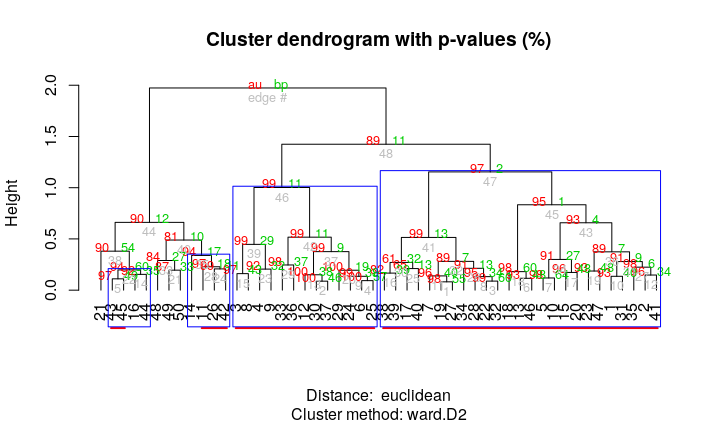
\includegraphics[width=1.00000\textwidth]{agrupamiento_dendrogramas_porcentajes.png}
\caption{mapa de la isla Barro Colorado dendrogramas y porcentajes
\label{fig:bci_map}}
\end{figure}

En el dendrograma anterior, también pueden notarse las probabilidades
por el método Ward (ver figura \#\#21)

Los dendrogramas, al igual que en los métodos de medición de asociación
permiten ver gráficmanete la dinámica de la distribución de las especies
de moraceae, sin embargo, estos nos ayudan a segmentar en grupos los
sitios con mayor cantidad de individuos o especies, dividiendolos en
cuadros a una mayor o menor altura, sería una forma de fraccionar en
grupos representativos lo que en principio parece desordenado y
monótono.

\subsection{Análisis de Variables Ambientales y
Mapas}\label{anuxe1lisis-de-variables-ambientales-y-mapas}

Dentro del análisis de agrupamiento, se haya incrustado el estudio de
las variales ambientales y los mapas. Desde un principio, en este
artículo, tanto la riqueza global como la de mi familia, han presentado
unos valores altos, y unos patrones de concentración y desplazamiento
por igual grandes.

Así se puede visualizar en el siguiente mapa (ver figura \#\#22)

\begin{figure}
\centering
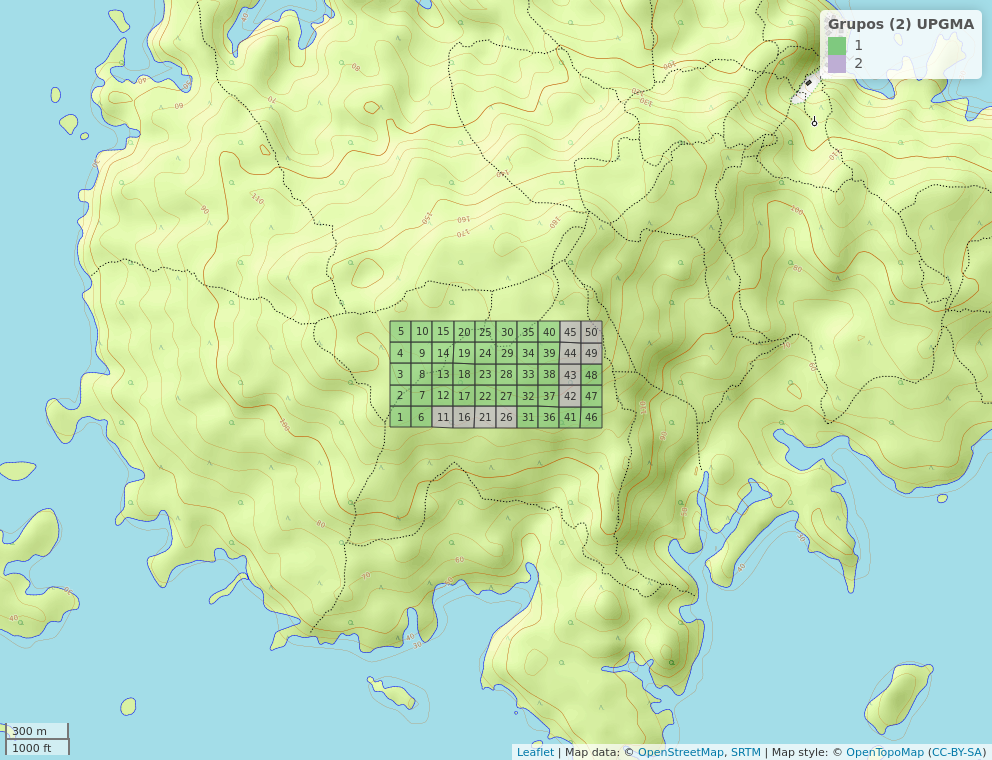
\includegraphics[width=1.00000\textwidth]{mapa_upgma_k2.png}
\caption{mapa de la isla Barro Colorado sitios de composición por
distancia de cuerda \label{fig:bci_map}}
\end{figure}

\begin{figure}
\centering
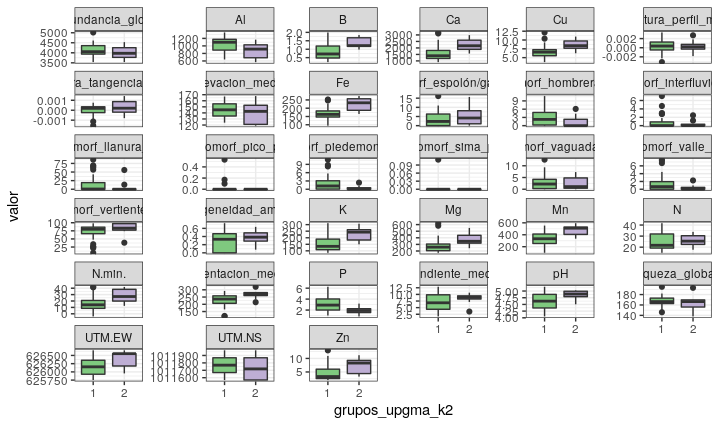
\includegraphics[width=1.00000\textwidth]{mapas_variables_ambientales.png}
\caption{mapa de la isla Barro Colorado mapa de variables ambientales
\label{fig:bci_map}}
\end{figure}

En el mapa adjunto, así como en el diagrama de cajas (ver figura
\#\#23), puede visualizarse el comportamiento de la mediana de las
variables ambientales, de la riqueza, así como también de abundancia. El
método UPGMA, presenta un patrón de distribución al este y al sur para
el grupo 2 de las variables ambientales dentro de la parcela de 50
hectáreas. Las varibles del grupo 1 de la parcela presentan un patrón en
todos los rumbos. Dentro de la riqueza, y la abundancia, los grupos 1 y
2, presentan valores no muy distantes, lo que evidencia el
condicionamieto ambietal de la isla, y que nuevamente refleja la fuerte
riqueza y asociación de las especies de Moraceae en dicho espacio
insular. Dentro de las variables ambientales de tipo geomorfológico, la
mediana para el grupo 1, naturalmente presenta mayores valores que
aquellos sitios de la misma parcela que se presentan en el grupo 2, pero
en cuanto a la concentración de elementos químicos en un número de
hectáreas más reducido (en este caso el grupo 2), representan mayor
valor para la mediana.

\begin{figure}
\centering
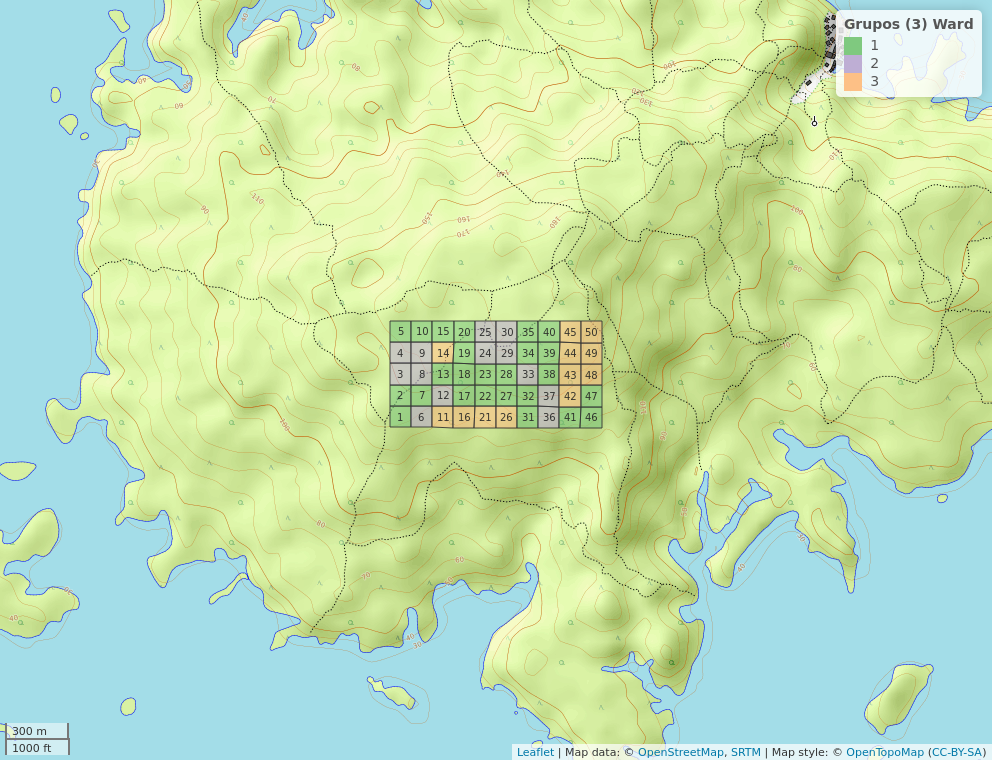
\includegraphics[width=1.00000\textwidth]{mapa_ward_k3.png}
\caption{mapa de la isla Barro Colorado grupos Ward k3
\label{fig:bci_map}}
\end{figure}

\begin{figure}
\centering
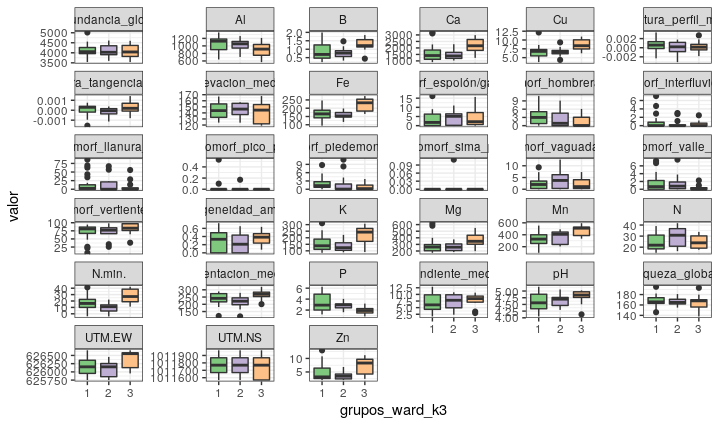
\includegraphics[width=1.00000\textwidth]{cuadro_cajas_ward.png}
\caption{mapa de la isla Barro Colorado cuadro de cajas Ward
\label{fig:bci_map}}
\end{figure}

Para el método Ward en el comportamiento de las varibles se presentan
tres sitios que muestran la dinámica de las variables ambientales dentro
de la parcela de 50 hectáreas con un patrón de distribución distinto al
caso anterior. Cuando relacionamos las varibles del diagrama de cajas
(ver figura \#\#25) que también se aprecian en el mapa (ver figura
\#\#24), puede corroborarse que estas se concentran más al centro de la
parcela, algunas al sur, y otras al este. Variables como el pH,
presentan altos valores de mediana en casi todas las hectáreas de la
parcela. También ocurre lo mismo con el nitrógeno. Para el caso de la
abundancia y la riqueza el valor de la mediana presenta valores
elevados, aunque en el caso de la primera las cajas o sitios ocupan
mayor espacio.

\subsection{Especies Indicadoras}\label{especies-indicadoras}

Para las especies indicadoras, tenemos que por especie indicadora se
entiende el grado de predicción que esta tenga dentro de un espacio bajo
estudio. Pueden darse casos de abunancia, y esos ejemplos de abundancia,
nos pueden llevar a la cocepción de grupos dentro de una familia. Dichos
grupos tienden a identificarse por el predominio de una variable
ambiental, ya sea un tipo de bosque, una concentración de pH, o de
ntrógeno. La aparición de estos grupos bajo el condicionamiento de
dichas variabes es lo que hace posible la existencia ordenada de los
mismos.

Existe el análisis de especies indicadoras por medio del método de
Inval, este método se aplica tanto para UPGMA, así como para Ward, se
verifica cuál es la especie que presenta el mayor indicador o
estadístico, la abundancia y la permutación. Para UPGMA, en el caso de
las Moraceae se registran dos grupos de una y cuatro especies
respectivamente. En el caso del primer grupo sería \emph{Perebea
xanthochyma} con una abundancia de 226, y un indicador (Inval) de 0.32,
tenemos en el segundo grupo: \emph{Pulsenia armata}, cuya abundancia es
de 993, y su indicador 0.774, \emph{Ficus tonduzzi} 23 y 0.459,
\emph{Tropis caucana} 136 y 0.454, y \emph{Tropis racemosa} con 218 y
0.420. En este primer grupo la especie indicadora es \emph{Perebea
xanthochyma} con los valores indicados y una permutación de 0.037, en el
segundo grupo: \emph{Pusenia armata} es la especie predictora de este
grupo por la abundancia que presenta, con un valor de permutación igual
0.001. El intervalo de confianza es pequeño, por ejemplo para
\emph{Brosimun alicastrum} va de -0.3597668 (-0.36) a 0.2896983 (0.29).

En el caso Ward, se registran por igual dos grupos, el grupo 3 y el
grupo 4 que resultaría de la suma del 2 y el 3 y que contiene una
especie indicadora. Sus valores de de abundancia e indicador estadístico
respectivamente son: \emph{Poulsenia armata} 993 y 0.785, \emph{Trophis
caucana} 136 y 0.538, \emph{Trophis racemosa} 228 y 0.435, y \emph{Ficus
tonduzii} 23 y 0.417.

Para el segundo grupo, tenemos la \emph{Maquira guianensis} con 1315 y
0.575. Para el tercer y cuarto grupo, las especies indicadoras son:
\emph{Pulsenia armata}, y para el cuarto grupo \emph{Maquiara guinensis}
con valores de permutación de 0.001 para ambos casos. Para el caso Ward
el intervalo de confianza es para la misma \emph{Brosimun alicastrum},
desde su límite inferior con -0.1289961 (-0.129) hasta su límite
superior de 0.41576092 (0.42).

\subsection{Análisis de Diversidad Alpha y
Beta}\label{anuxe1lisis-de-diversidad-alpha-y-beta}

En este artículo se emplean dos modalidades de estudio: Alpha y beta.

Para la diverisdad alpha sobre la familia en cuestión se muestran los
resultdos siguientes,

\begin{figure}
\centering
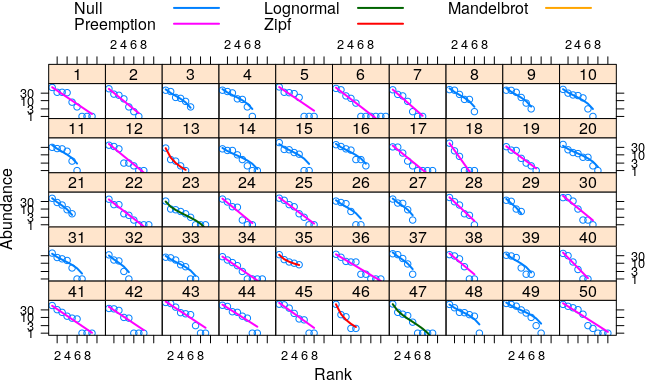
\includegraphics[width=1.00000\textwidth]{modelo_abundancia_especie.png}
\caption{mapa de la isla Barro Colorado modelo abundancia de especies
\label{fig:bci_map}}
\end{figure}

La gráfica anterior (ver figura \#\#26) representa la abundancia por
sitios, sitios de una hectárea, pero cada línea representa una métrica.
El gráfico también presenta cuáles sitios podrían mostrar mayor equidad.
Encontramos que las líneas de color verde y azul represental la mayor
abundancia de los lugares en los cuales se encuentran.

\begin{figure}
\centering
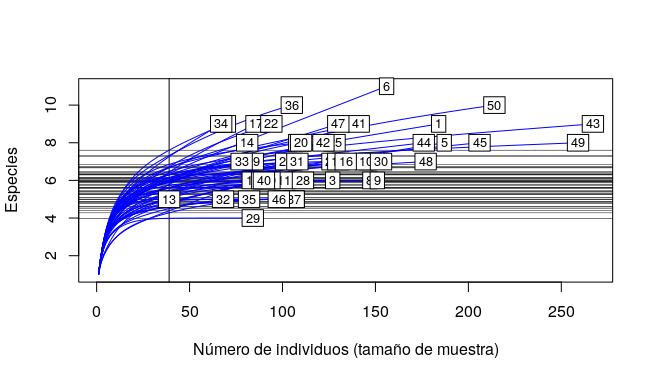
\includegraphics[width=1.00000\textwidth]{Numero_individuos.png}
\caption{mapa de la isla Barro Colorado número de individuos
\label{fig:bci_map}}
\end{figure}

En el digrama anterior (ver figura \#\#27) de curvas de rarefacción
puede apreciarse también el número de individuos por sitios. En este
diagrama puede apreciarse que prácticamente la totalidad de de sitios
poseen una cantidad de individuos superior a los 50 individuos, con
excepción del sitio 13 que posee unos 45 aproximadamente, y un escaso
número de sitios con una catidad superior a los 200 individuos. La mayor
cantidad de sitios comprende una riqueza en especies que va de los 50 a
los 200 individuos.

\subsection{Diversidad Beta}\label{diversidad-beta}

La diversidad beta se puede apreciar en segiente mapa de cuadros (ver
figura \#\#27), seguido de la gráfica (ver figura.

\begin{figure}
\centering
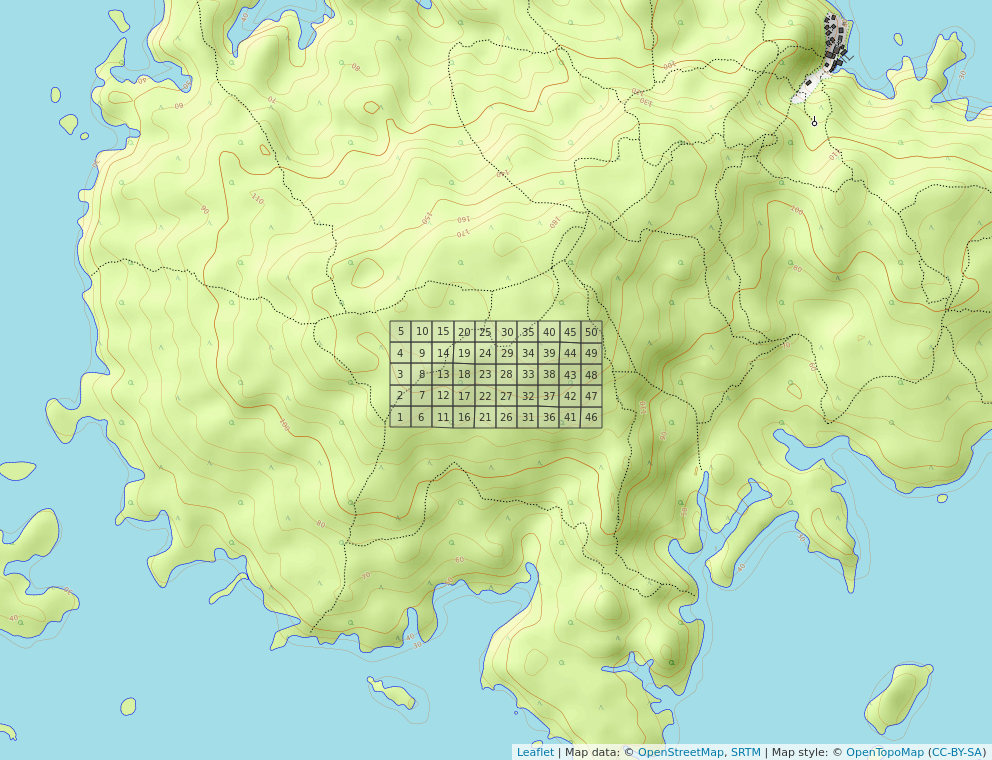
\includegraphics[width=1.00000\textwidth]{mapa_cuadros.png}
\caption{mapa de la isla Barro Colorado mapa cuadro diversidad beta
\label{fig:bci_map}}
\end{figure}

\begin{figure}
\centering
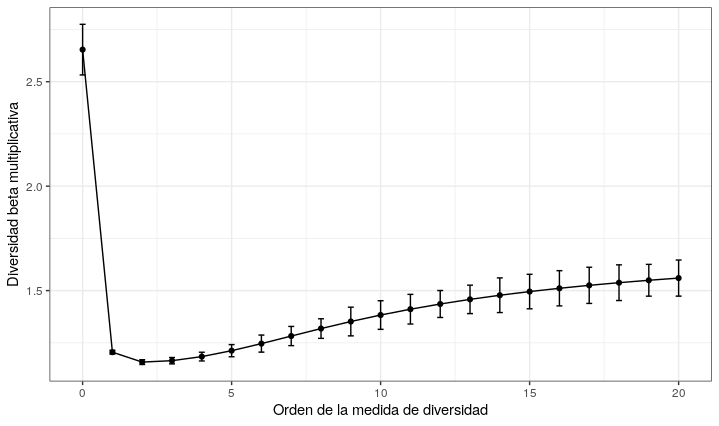
\includegraphics[width=1.00000\textwidth]{diversidad_beta.png}
\caption{mapa de la isla Barro Colorado mapa de calor
\label{fig:bci_map}}
\end{figure}

Para este tipo de diversidad, se presenta un patrón de distribución al
este de la parcela de 50 hectáreas y se aprecian las parcelas de una
hectárea que poseen la mayor cantidad de individuos por especies, al
oeste se aprecia una diversidad mucho más reducida. Este modo de
visualizar la variabilidad es más comprensible que en los casos
anteriores. En el gráfico (ver figura \#\#28) también puede apreciarse
mayor diversidad al este de la parcela.

\subsubsection{Análisis de Ordenación Simple (no restringida y
restringida)}\label{anuxe1lisis-de-ordenaciuxf3n-simple-no-restringida-y-restringida}

Las principales técnicas de análisis no restringido son: PCA (Análisis
de Componentes Principales), CA (Análisis de Correspondencia), PCoA
(Análisis de Coordenadas Principales), y NMDS (Escalamiento
multidimesional No Métrico).

Así se muestran para la familia de moraceae, empleando la técnica de
escalamiento PCA, la cual compara las componentes principales.

\begin{figure}
\centering
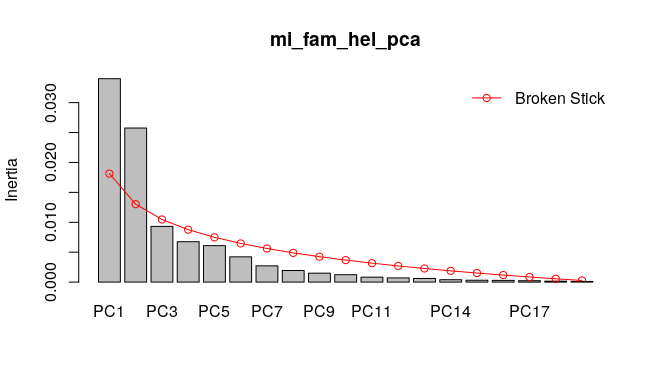
\includegraphics[width=1.00000\textwidth]{mi_fam_hel_pca.png}
\caption{mapa de la isla Barro Colorado diagrama de componentes
principales variables\label{fig:bci_map}}
\end{figure}

En este diagrama de componentes principales se puede visualizar un
decenso brusco de la medida de la inercia que pasa de 0.030 en la
componente principal 1 a 0.00 en la componente princioal 17 (ver figura
\#\#29).

\begin{figure}
\centering
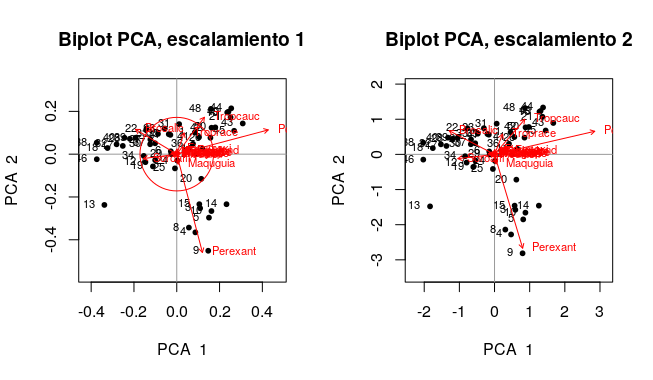
\includegraphics[width=1.00000\textwidth]{escalamiento_1_2.png}
\caption{mapa de la isla Barro Colorado diagrama de escalamiento 1 y 2
\label{fig:bci_map}}
\end{figure}

En esta técnica de escalamiento pueden visualizarse los grados de
asociación mediante un plano de coordenadas ortogonales. La cercanía que
describen los ángulos de las variables ambientales representa el grado
de asocición de las mismas. En el primer cuadrante (ver figura \#\#30)
predomina la distancia euclídea, en el segundo, la distancia de
Mahalanovich. Se forman nuves de puntos en los cuadrantes, estos puntos
representan los sitios, y como se puede ver en los gráficos, estos se
concentran más en el cuadrante negativo. Para ambos casos hay mayor
asociación al norte del plano.

\begin{figure}
\centering
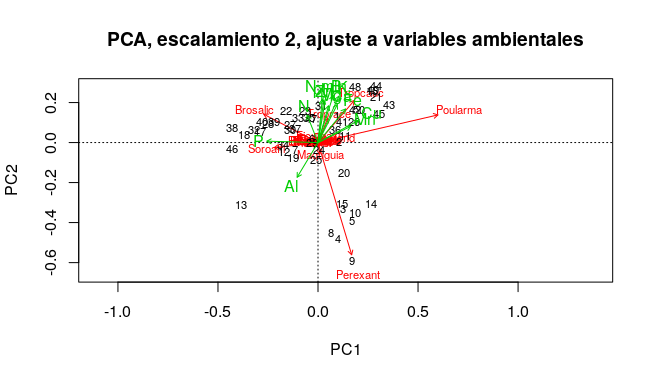
\includegraphics[width=1.00000\textwidth]{escalamiento_ajuste_2.png}
\caption{mapa de la isla Barro Colorado diagrama asociación de
variables\label{fig:bci_map}}
\end{figure}

En este diagrama (ver figura \#\#31) puede percibirse la fuerte
asociación que existe en las variables ambientales (color verde), por la
cercanía de los ángulos en la parte superior del plano. Hay mayor
asociación en la componente principal 2 que en la componente principal
1.

\subsubsection{Ordenación Simple
Restringida:}\label{ordenaciuxf3n-simple-restringida}

Para la ordenación restringida, las tendencias asociadas a un grupo de
ordenación se asocian a otro grupo. Las principales técnicas de
ordenación restringida son: Análisis de redundancia (RDA), Análisis de
redundancia basado en la distancia (db-RDA), Análisis de Correspondencia
Canónica (CCA), Análisis Discriminante Lineal (LDA), Curvas de
respuestas Principales (PRC), Análisis de Correspondencia conjunto
(CoCA, Análisis de Correlación Canónica (CCorA) y Análisi de Inercia
Conjunto (ColA).

En esta parte se mostrarán los resultados para RDA Y CCA. RDA combina la
regresión y elanálisis de componentes principales.

\begin{figure}
\centering
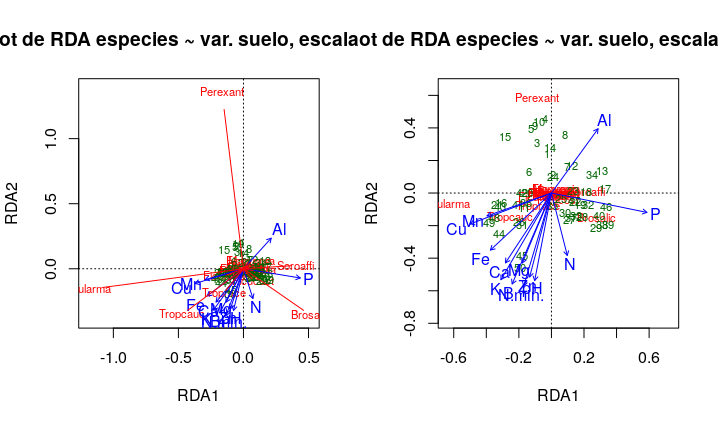
\includegraphics[width=1.00000\textwidth]{rda_escala_especies.png}
\caption{mapa de la isla Barro Colorado RDA diagrama de especies
variables\label{fig:bci_map}}
\end{figure}

\begin{figure}
\centering
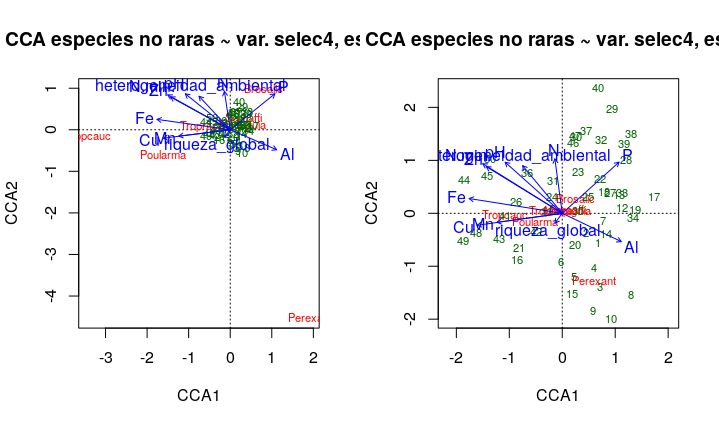
\includegraphics[width=1.00000\textwidth]{rda_escalamiento_escala_5.png}
\caption{mapa de la isla Barro Colorado RDA especies no raras
variables\label{fig:bci_map}}
\end{figure}

\begin{figure}
\centering
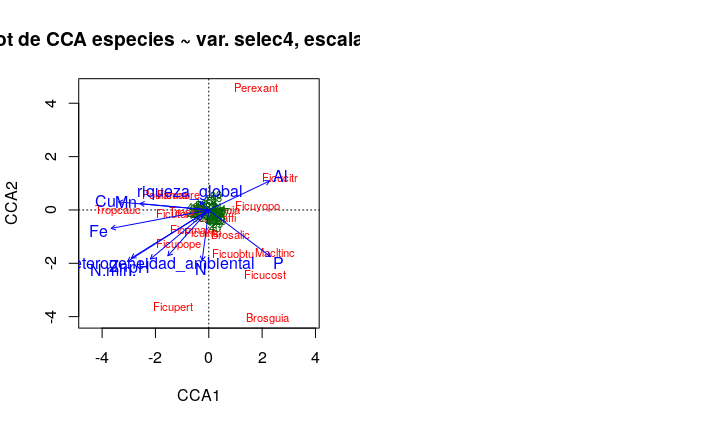
\includegraphics[width=1.00000\textwidth]{rda_especies_escala_4.png}
\caption{mapa de la isla Barro Colorado RDA digrama de especies
variables\label{fig:bci_map}}
\end{figure}

En estos planos bidimensionales puede apreciars el comportamiento de las
variables ambientales incluyendo el recurso suelo, de las especies, y de
especies no raras. en el primer diagrama (RDA) (ver figura \#\#32) puede
verse la fuerte asociación de los elementos químicos que integran el
suelo, descrita por las líneas azules que represental los ángulos en el
tercer cuadrante del plano. En el digrama de especies no raras (CCA)
(ver figura \#\#33) se percibe una fuerte concentración de sitios en el
tercer cuadrante, y es precisamente allí donde existe una menor
asociación entre elementos químicos (variables ambientales). Por ejemplo
el fósforo está presente en la mayor cantidad de sitios, y es un
elemento que se encuentra a una distancia angular considerada con
relación a los demás, lo mismo pasa con el alunminio. Para el cobre, el
manganeso y el hierro ocurre todo lo contrario.

En el último diagrama (ver figura \#\#34) correspondiente a CCA, existe
mayor asociación entre las especies en las zonas con predominio de
fósforo y aluminio, correspondiete a los cuadrantes 1 y 2 del plano.

\subsection{Análisis Espacial de Datos Ecológicos
(Autocorrelación)}\label{anuxe1lisis-espacial-de-datos-ecoluxf3gicos-autocorrelaciuxf3n}

Esta es una froma de observar los valores de las variables Ambientales
desde una perspectiva espacial, por medio de segmentos verticales,
parecidos a bastones, encerrados en cajas, se pueden ver de una forma
más comprensiva la dinámica del valor de correlación de las especies de
Moraceae que se vienen tratando, y que se pueden apreciar en el gráfico
o correlograma (ver figura \#\#35).

\begin{figure}
\centering
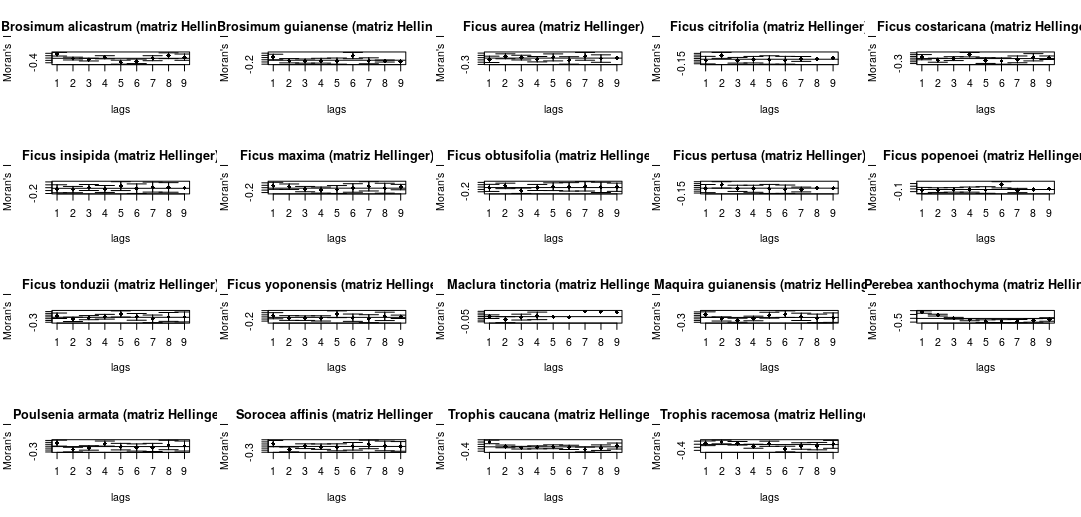
\includegraphics[width=1.00000\textwidth]{multiples_especies.png}
\caption{mapa de la isla Barro Colorado RDA digrama de especies
variables\label{fig:bci_map}}
\end{figure}

A partir de esta pequeña descripción del correlograma se puede entender
la dinámica espacial de algunas especies de Mooraceae. Como puede verse
existe una correlación más positiva que negativa entre las distintas
especies de moraceae. Lo que nuevamente viene a recrear la gran riqueza
predominante en las distintas especies de Moraceae, la similaridad qe se
hace visible en cada modo de estudio empleado.

\section{Discusión}\label{discusiuxf3n}

La abundancia y riqueza de la familia Moraceae, dentro de la isla Barro
Colorado, es vieja y asentada en terreno bajo, en su generalidad, con
una adaptación bastante ajustada a las condiciones de los factores
físico químicos de dicha isla, por lo general son plantas perennes, de
gran porte que sirven de alimentación a los individuos frugívoros que
allí habitan, constituyendo con su dosel el típico paisaje de la selva
tropical crentroamericana.

Como se pudo ver en los mapas, y los cuadros de variables, se presenta
gran riqueza y abundancia en espacios muy reducidos. Todo esto nos hace
pensar que se trata un gran bioma en miniatura en el que se reducen las
distancias, y se incrementan los ejemplares que hacen confluir la
biología y la geografía. Tal vez en el aspecto geomorfológico no se
puedan hacer conjeturas similares. Pero desde la biogeografía, el
sendero es complejo. El hecho de que exista este conglomerado de
especies de plantas y animales, requiere de unas condiciones óptimas
para hacer posible la vida de este gigantesco ecosistema. En los mapas
de abundacia, tanto global como de la familia se advierte un crecimiento
casi perfecto, bajo condiciones físicas y químicas que le son favorables
a la vida en esta parte del mundo.

No se ignora que a la misma latiud se encuentren condiciones similares
en otros rincones de la tierra, de hecho las zonas intertropicales, las
tropicales y las ecuatoriales se caracterizan más por la riqueza que por
la abundancia. Pero en ese sentido tenemos millones de kilómetros bajo
estudio si nos adentraramos en las grandes selvas que se conocen de
antiguo, y tal vez nos toparíamos más con abundancia que con riqueza.
Las grandes expediciones de la historia se han distinguido siempre por
cubrir amplios itinerarios, que a su vez implican grandes distancias.

Dentro de la selva del ístmo, BCI, es como un estracto sintético
susceptible de múltiples investigaciones, por su amplia concentración de
flora y fauna. Si bien la isla Barro Colorado es un enclave marítimo, y
de investigación científica, contando por ende con las riquezas antes
descritas, es motivo de cuestionamiento, el cómo un espacio, esta
pequeña isla, haya acumulado estas riquezas en tan poco tiempo, a
sabiendas de la zona geoastronómica en que se encuentra. Sería más
aceptable la abundancia.

La construcción de riquezas ecológicas, ademas del emplazamiento
geográfico, requieren de eventos geológicos, geográficos y tal vez
antrópicos, en este caso tenemos el Canal de Panamá, el recuerdo mejor
conservado de la injerencia yanqui en el Caribe. Una isla que se formó
en algo más de un siglo, pues de la misma forma corre el riesgo de
desaparecer. Pero esto solo compete a un asunto geológico, que no
concierne a este trabajo, solo de manera parcial.

En el caso de la pendiente, esta es favorable para formaciones boscosas
como la que he asumido, aunque inservible para la agricultura bajo
cualquier consideración que se haga a favor de la vegetación que no sea
referente a la anteriormente citada. Sin embargo la altitud guarda una
relación acorde con las dimensiones de la isla. Las plantas como las
Moraceae mantienen una relación favorble con estos grados de inclinación
del terreno. Ya en espacios controlados y con plantaciones con las qe se
persigue un determinado propósito se tiene un conocimiento sobre el
manejo de la pendiente, a sabiendas de que en este escenario han crecido
de forma silvestre sin intervención alguna de la mano del hombre.

La isla constituye uno de los ecosistemas más grandes del mundo, lo que
deja al descubierto la gran adaptabilidad que presentan algunas plantas
a este medio. Por tratarse de un lugar sumamente pequeño, los rasgos
orográficos han de ser casi imperceptibles, pero sobre todo la edad de
la isla no la hace poseedora de formas del relieve que estén
consolidadas dentro de lo ques es la periodización geológica. Pues la
isla se formó hace algo más de un siglo, tiempo en el qe no caben
eventos geológicos trascendentales.

BCI constituye como una especie de interrupción del sistema orgráfico de
la región istmica panameña y centroamericana, pues la espina dorsal de
toda la costa del Pacífico, aunque no se eleva de forma tan imponente
como en los Andes o en las Montañas Rocosas, en Centro América, poseen
continuidad, aunque con una escasa altiud. Es como si se tratara de un
lugar construido para la investigación, en medio de sistemas tan
extremos, es decir franja estrecha de tierra y masas imensas de agua que
aguardan a ambos lados del Canal de Panamá (situación ístmica).

La familia de plantas que nos interesa sobreabunda en estas condiciones.
Muy probablemente las familias de Moraceae presentes en otros lugares
prosperen bajo condiciones muy diferentes. Sin embargo los lugares a una
misma latitud en el planeta, se caracterizan por operar sobre los
indiviuos bajo las mismas condiciones, por ende las condiciones de pH en
otras regiones tal vez no se alejen tanto de las que por el momento se
citan.

El pH es un factor que en lo adelante incidirá en la utilidad de la
planta, especialmete a nivel comercial, la presencia de uno o varios
elementos, o la ausencia de estos determinará el valor utilitario de
estas. La quimiotaxonomía o qimiosistemática evalúa la presencia de
elementos químicos en especies vegetales, el aspecto químico de la
clasificación de las plantas, se basa en sus constituyentes es decir en
sus características moleculares. Estas al igual que las características
geomorfológicas son controladas químicamente.

Dentro los factores físico químicos las medidas de pH no suelen presetar
cambios significativos, en las inmediaciones de las aguas del Canal de
Panamá, pese a que se presentan ligeras fluctuaciones en las medidas de
este indicador, que en esencia muestran la sensibilidad de las aguas
circundantes, este por lo general es regular (Simmonds, Gómez, \&
Villalaz, 2002,). Esto sugiere un grado de adaptabilidad bastante
desarrollado por las especies de la familia en cuestión, no solo al
medio de la isla, sino tambien de las áreas circundantes. La fenología
reprodctiva de la Isla de Barro Colorado ha sido descrita extensamente
por algunos autores. Los árboles más grandes presentan un pico de
floración entre febrero y junio, y alcanzan un máximo en marzo y abril,
justamente al final de la estación seca (Williams-Linera \& Meave,
2002,). Tal vez este régimen de floración y de adaptación permitan a las
Moraceae mantener una fenología por encima de los patrones físico
químicos, en este caso especialmente el pH.

Como pudo verse en los demás bloques que corresponden a las mediciones
de asociación, análisis de agrupamiento jerárquico, diversidad,
ordenación, y análisis ecológico espacial. La fuerte asociación
prevalece en las especies de Moraceae. Algunas variables ambientales
como el pH mantienen sun primacía en su modalidad ácida. Pero en todo
este trabajo, lo que generalmente prevalece es la similaridad entre
sitios que contienen especies, denotado en los diferentes métodos
empleados y en las matrices descritas, existe una fuerte cohesión entre
individuos similares y abundantes en espacios sumamente reducidos.

Las Matrices de Hellinger, de Spearman, así como la distancia de
Jaccard, vienen a hacer síntesis de los niveles de asociación
predominantes en la parcela, determinando la disimilaridad, y la
similaridad y los contrastes que existen cuando se emplean otros
métodos.

Nuestro interés se centra, en esta parte, en las condiciones que han
creado este espacio insular tan singular, en un tiempo tan breve, en el
istmo de Panamá. Si bien sabemos que América es la masa continental que
alcanza mayor extensión latitudinal, es probable que en todo el tiempo
precedente a la construcción del canal, se dieran las migraciones de
especies tanto del norte como del sur. Aunque, una vía interoceánica
artificial como lo es el Canal de Panamá, probablemente no provocaría
cambios notables en el equilibrio biológico de las comunidades de
individuos que poblaban esta parte del continente.

La sostenibilidad de las especies de plantas y animales que allí existen
no se puede poner en duda, por las condiciones climáticas que en dicho
lugar se mantienen. Es como si tratara de un ambiente controlado y
planificado. De modo que las investigaciones siempre tienen una página
que arañar, dando motivos de colgarse una mochila y salir a hacer
trabajo de campo. Es muy probable que para muchos, BCI siga siendo el
secreto mejor guardado dentro de las regiones de investigación más
llamativas del mundo,lo cual resulta ser asombroso por el peso que posee
el istmo de Panamá a escala comercial.

El presente artículo ha sido un intento por abordar la información
básica de la familia de las Moraceae, desde una perspectiva científica,
teniendo como escenario la isla de Barro Colorado. En el desarrollo me
he volcado más en lo que es la distribución de individuos por hectárea,
en una parcela de 50 hectáreas, tanto desde una perspectiva global, como
específica, en las condiciones del terreno, así como en la situación
geográfica, pretendiendo dar un enfoque lo más abarcador posible,
siguiendo estas variables, que han de ser de las más pertinentes para la
consideración de un trabajo de campo.

Sabemos que esta familia de angiospermas posee gran riqueza y abundancia
en esta parte del istmo, y que las condiciones típicas del suelo son
idóneas para su sostenimiento. En un principio mencioné el caso de otras
regiones próximas, por sus estadísticas en cuanto a predominio de
plantas, especialmete de la familia que estoy tratando.

Panamá es uno de los paises más diversos, ya que tiene el 10\% de la
fauna y flora global. México tiene el 11\%, pero Panamá cabe en México
unas 26 veces. Panamá tiene 1010 especies registradas, de esa cantidad
un tercio le corresponde a la isla Barro Colorado. El bosque de Barro
Colorado se cierra muy abajo y es difícil ver algunas especies de aves,
solo se pueden escuchar. Las especies de Moraceae por lo general
corresponden a árboles de hojas anchas (latifoliados), lo que hace de
los suelos de estas especies, lugares prácticamente impenetrables por la
radiación solar, algo típico de la selva en cualquiera de sus
denominaciones. En el bosque la temperatura promedio es de 27 grados
centígrados (80\(^\circ\) fahrenheit), y la humedad es bastante alta.

Existen muchos lugares en el Mar Caribe que como BCI, pueden ser grandes
laboratorios, a partir de los cuales se pueda hacer ciencia, producir
material científico de utilidad, pero la dependencia es peor que el
analfabetismo. Por ello tal val tenemos una ciencia estacionaria,
incapáz de dar el santo de la libertad.

Y se espera que el caudal de inforamción que se genera en las
investigaciones alcance a estos lugares, porque la ciencia genera
identidad a los lugares y los hace crecer. BCI, tiene algo más de 100
años, pero Panamá como nación es más vieja, y no es mi incumbencia el
tema político, ni de este artículo. Pero hago la aclaración porque
entiendo que se puede crecer en la ciencia, siempre dejando claro que
cada pueblo tiene contextos distintos y que el error siempre será tratar
de copiar. Este ha sido un trabajo en virtud del interés biológico, y
geográfico. Esperando que sea del agrado de quienes puedan leerlo.

\section{Agradecimientos}\label{agradecimientos}

Quiero dedicar todo mi agradecimiento, primero a Dios porque es quien
hace posible todas las cosas, luego al maestro José Ramón Martínez
Batlle, maestro de la escuela de ciencias geográficas en la facultad
ciencias de la Universidad Autónoma de Santo Domingo, en las áreas de
biogeografía, geomorfología, y anteriormente de geología por enrutarnos
en este mar de investigación que siempre termina arrojando cosas nuevas.
Por último a mis compañeros de carrera, Carolain Pérez Ureña, Ana Hilda
Valera, Darihanna Linares y Wilson Robles Rosario, sin ellos esto no
habría sido posible, muchas gracias.

\section{Información de soporte}\label{informaciuxf3n-de-soporte}

\begin{figure}
\centering
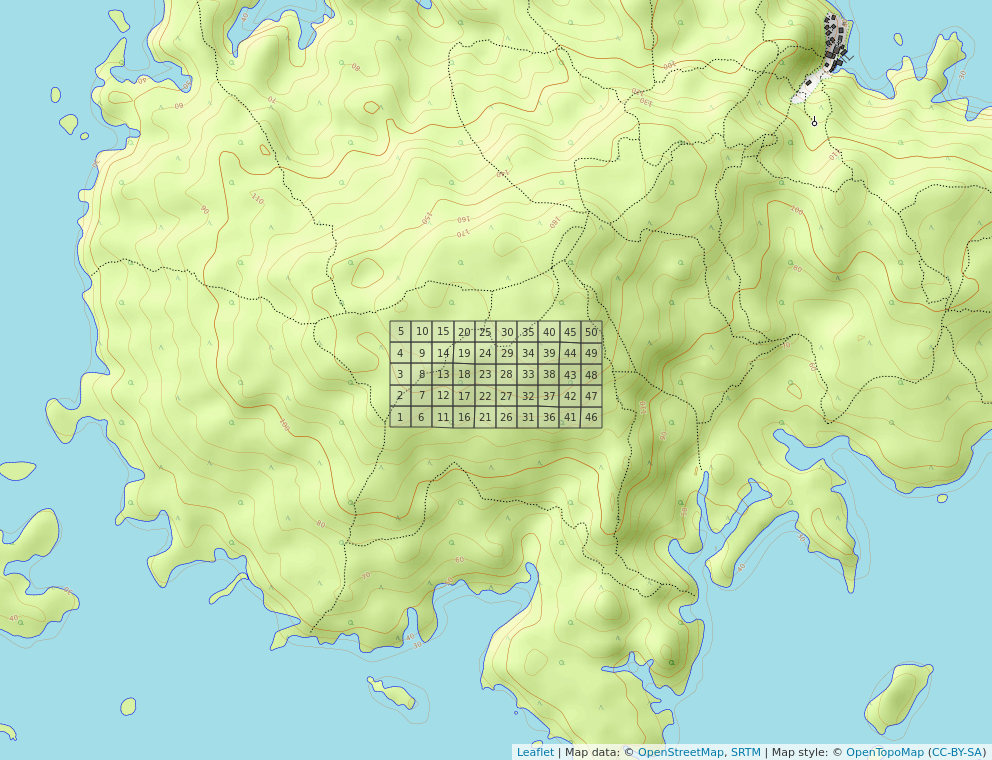
\includegraphics[width=1.00000\textwidth]{mapa_cuadros.png}
\caption{mapa de isla Barro Colorado cuadros\label{fig:bci_map}}
\end{figure}

\begin{figure}
\centering
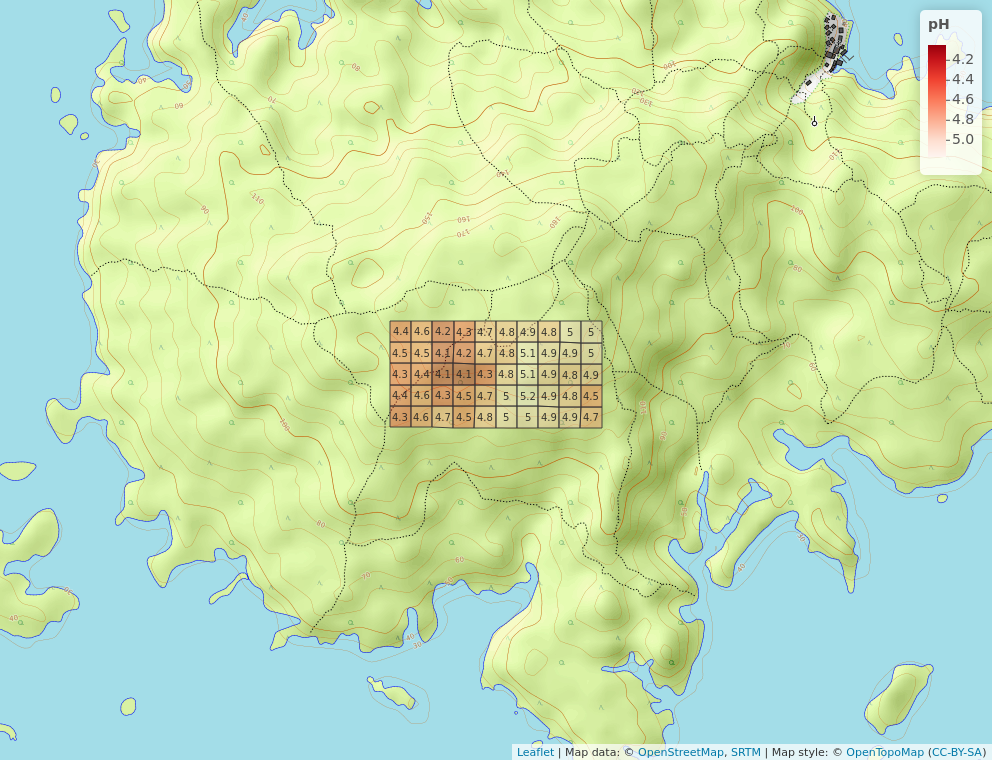
\includegraphics[width=1.00000\textwidth]{mapa_cuadros_ph.png}
\caption{mapa de la isla Barro Colorado cuadros ph\label{fig:bci_map}}
\end{figure}

\begin{figure}
\centering
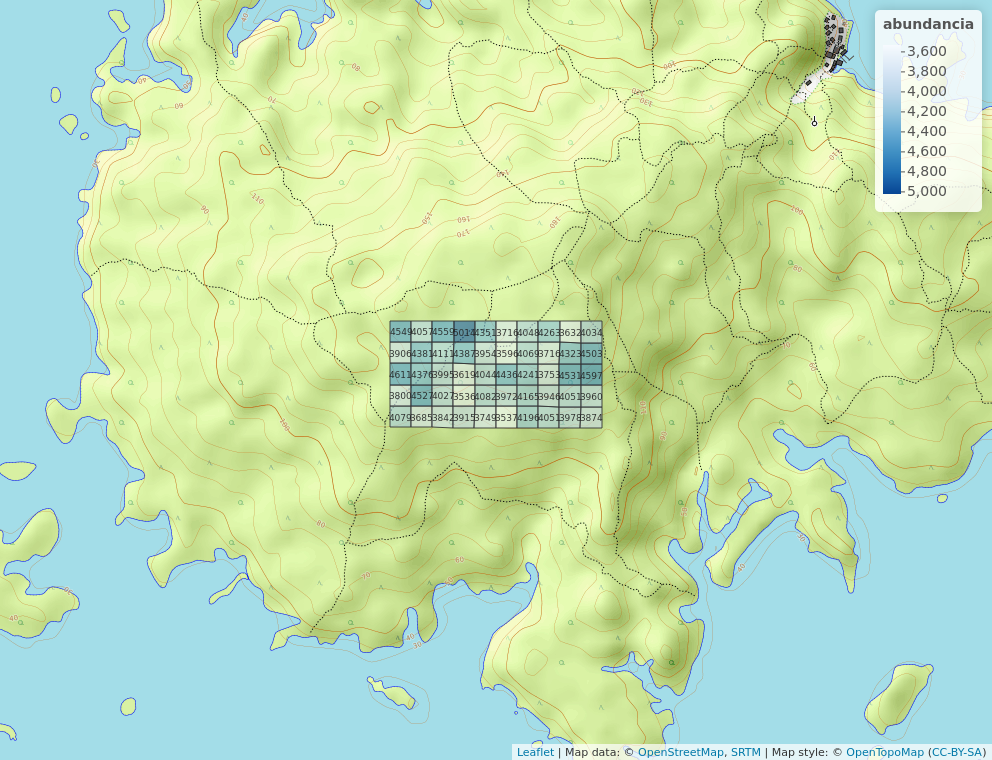
\includegraphics[width=1.00000\textwidth]{mapa_cuadros_abun_global.png}
\caption{mapa de la isla Barro Colorado abundancia global
\label{fig:bci_map}}
\end{figure}

\begin{figure}
\centering
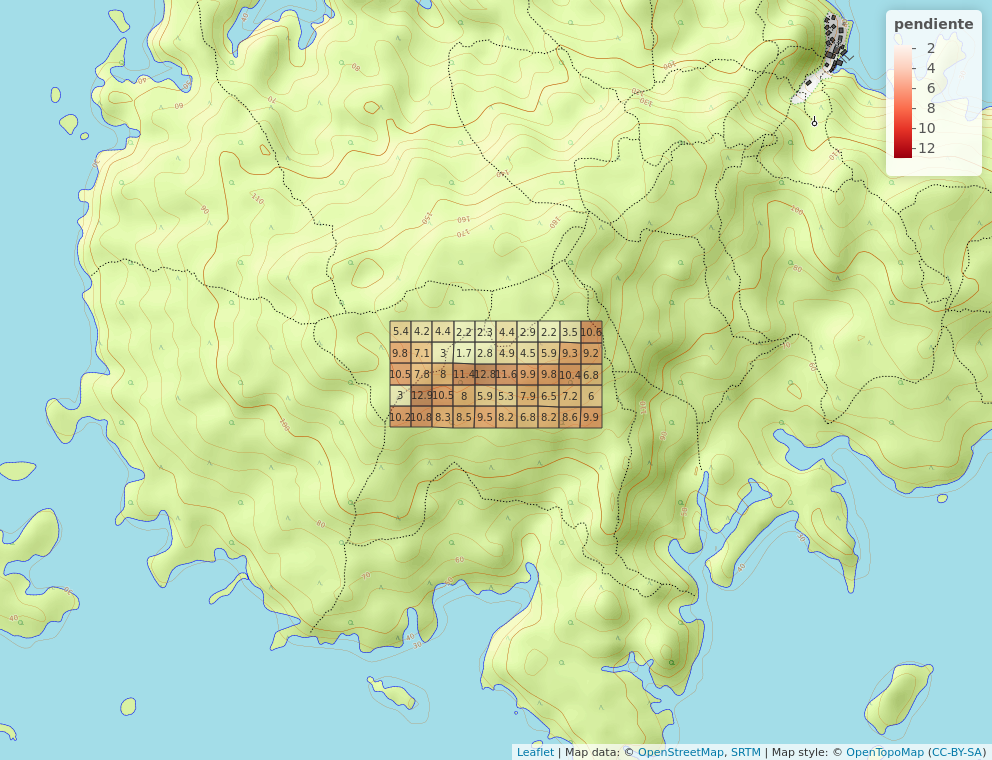
\includegraphics[width=1.00000\textwidth]{mapa_cuadros_pendiente.png}
\caption{mapa de la isla Barro Colorado cuadros y pendientes
\label{fig:bci_map}}
\end{figure}

\begin{figure}
\centering
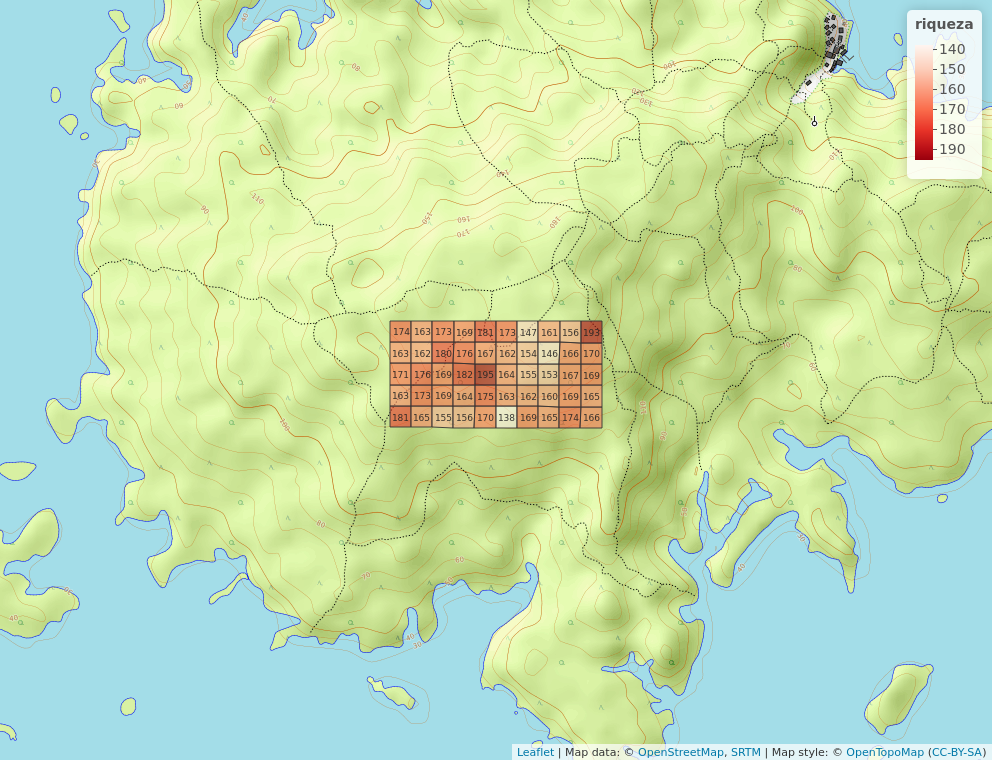
\includegraphics[width=1.00000\textwidth]{mapa_cuadros_riq_global.png}
\caption{mapa de la isla Barro Colorado riquza global
\label{fig:bci_map}}
\end{figure}

\begin{figure}
\centering
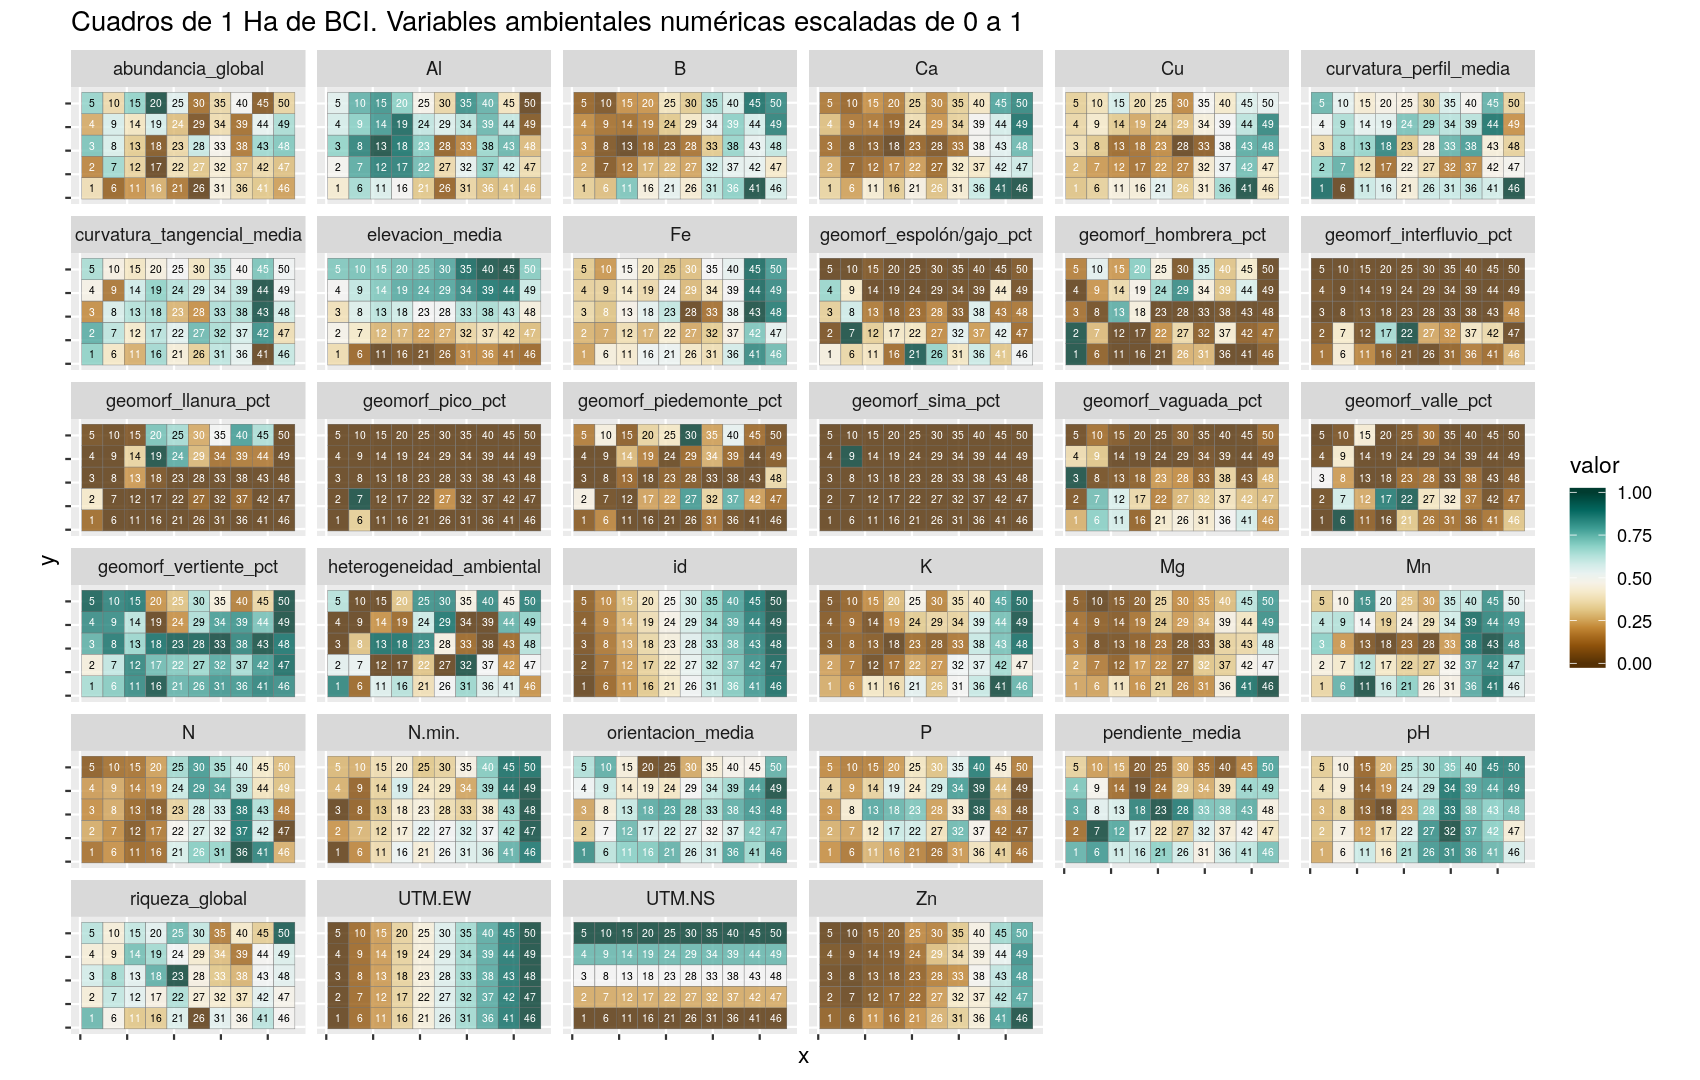
\includegraphics[width=1.00000\textwidth]{mapas_variables_ambientales_numericas.png}
\caption{mapa de la isla Barro Colorado variables ambientales numéricas
\label{fig:bci_map}}
\end{figure}

\begin{figure}
\centering
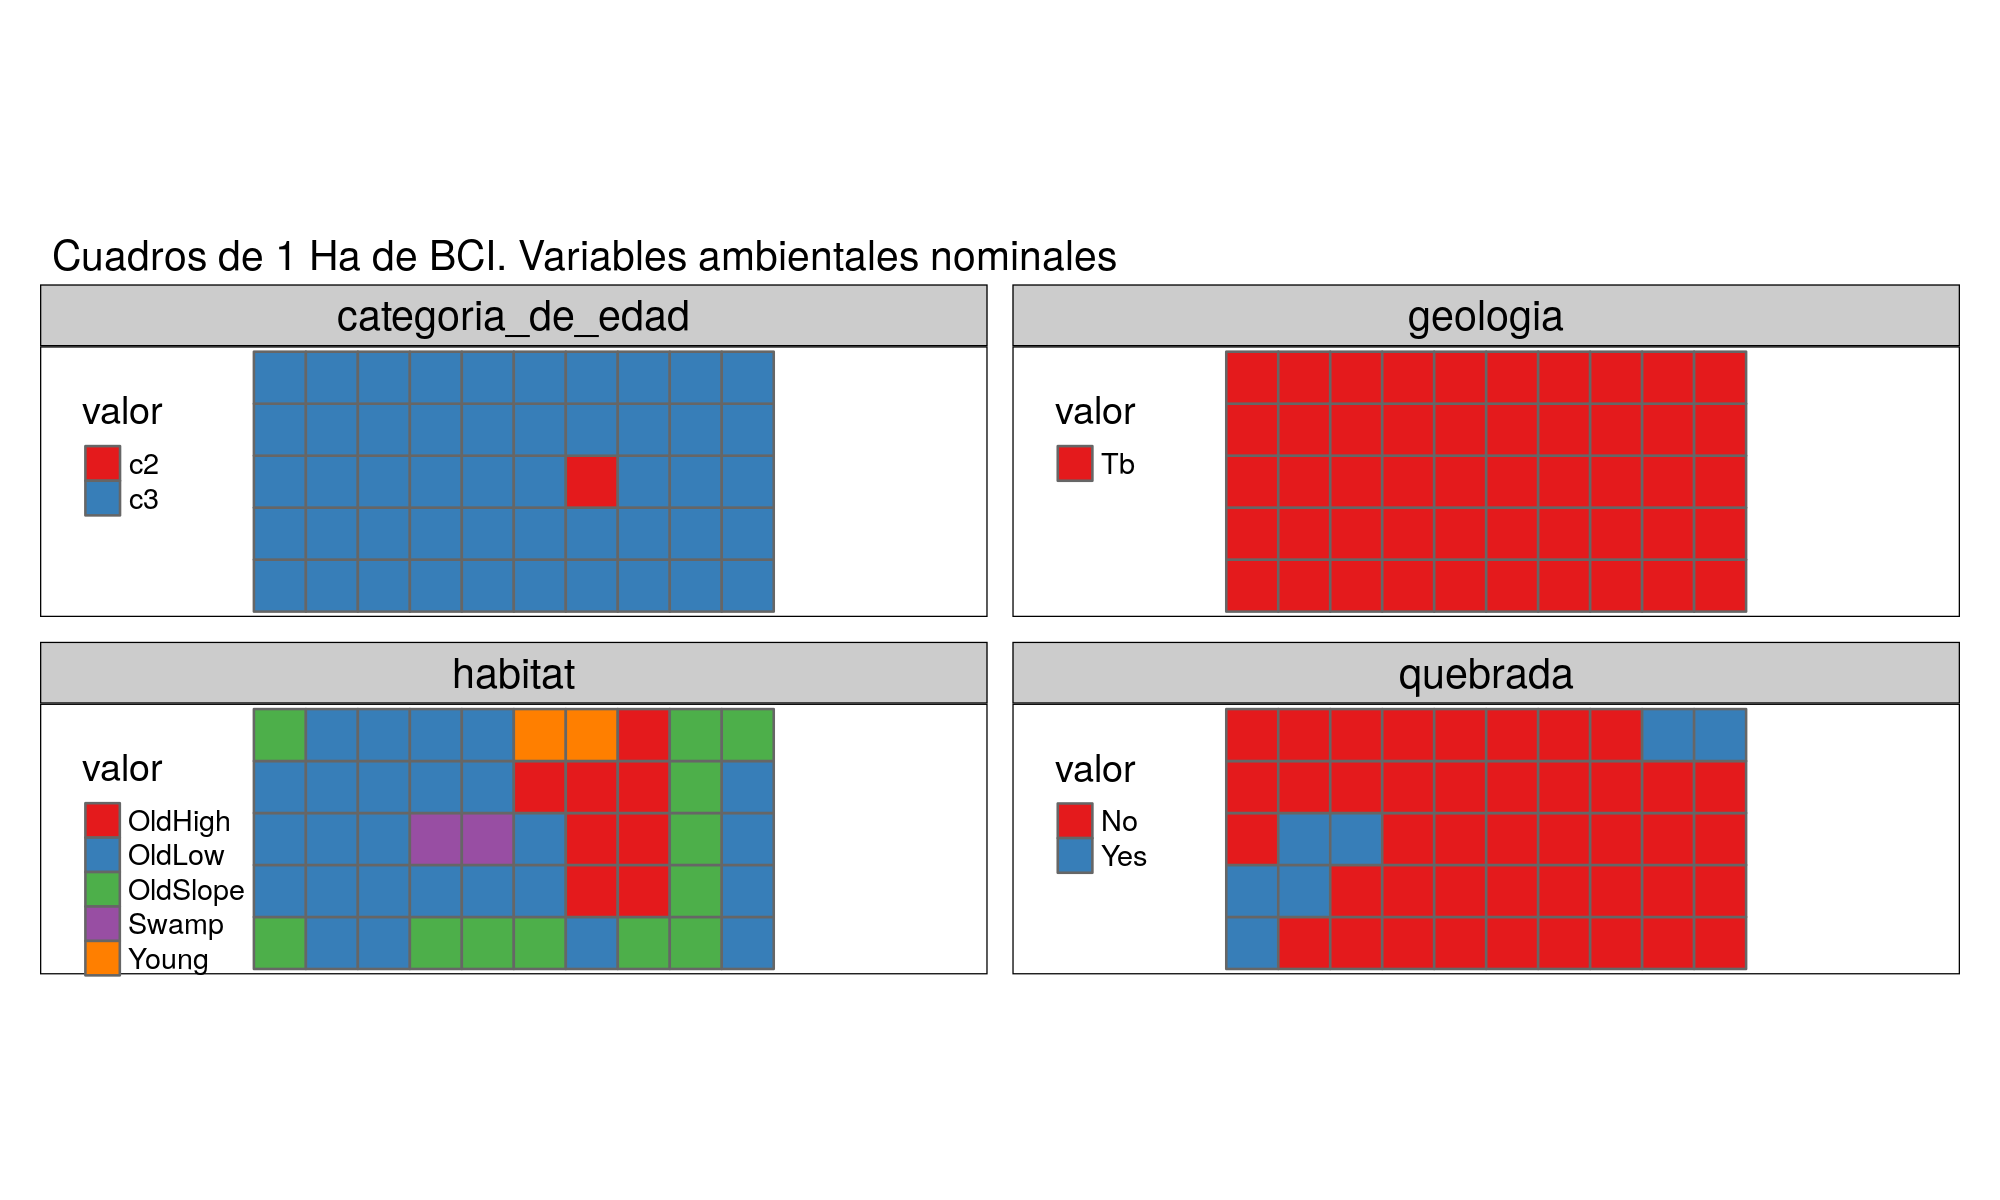
\includegraphics[width=1.00000\textwidth]{mapas_variables_ambientales_nominales_tmap.png}
\caption{mapa de la isla Barro Colorado variables ambientales nominales
\label{fig:bci_map}}
\end{figure}

\begin{figure}
\centering
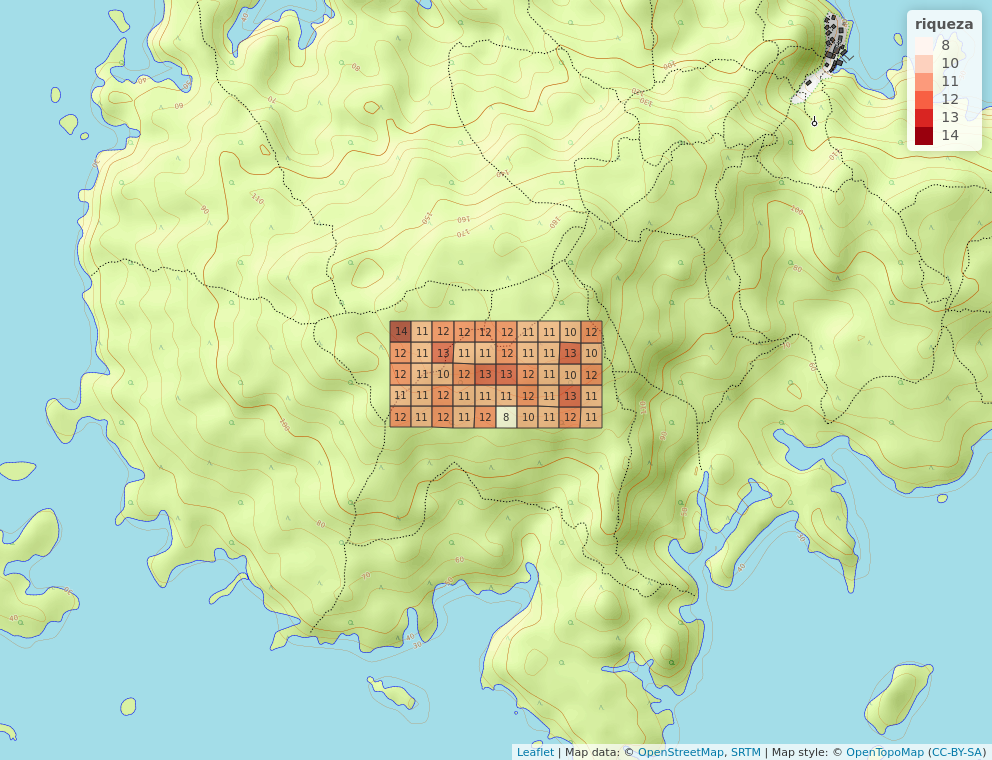
\includegraphics[width=1.00000\textwidth]{mapa_cuadros_riq_mi_familia.png}
\caption{mapa de la isla Barro Colorado cuadro de riqueza mi familia
\label{fig:bci_map}}
\end{figure}

\begin{figure}
\centering
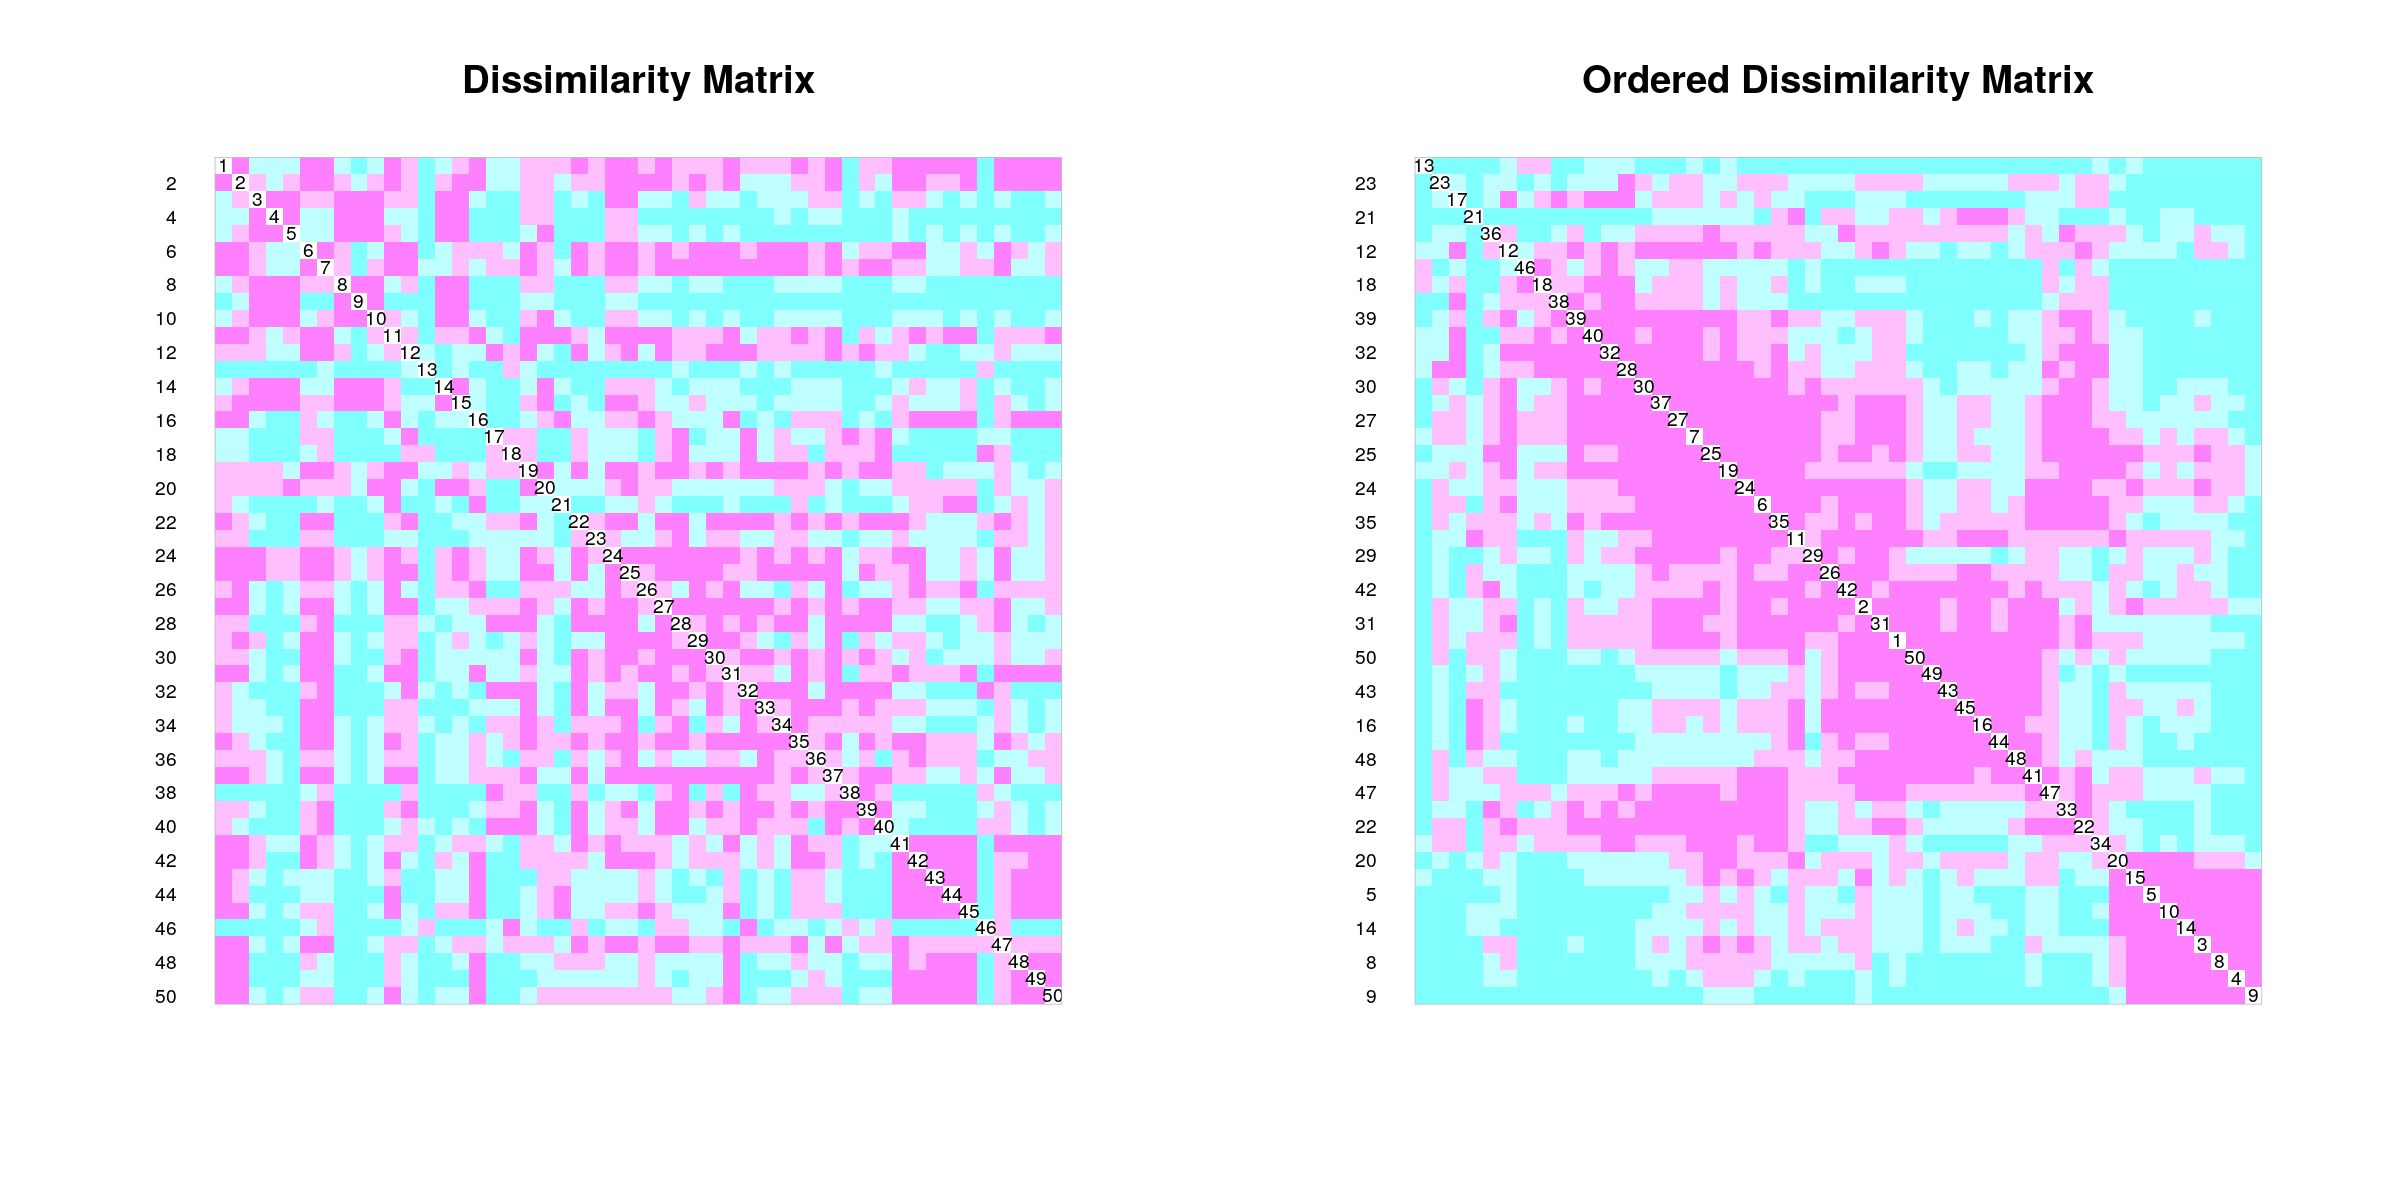
\includegraphics[width=1.00000\textwidth]{matriz_disimilaridad_hellinger.png}
\caption{mapa de la isla Barro Colorado matriz disimilaridad hellinger
\label{fig:bci_map}}
\end{figure}

\begin{figure}
\centering
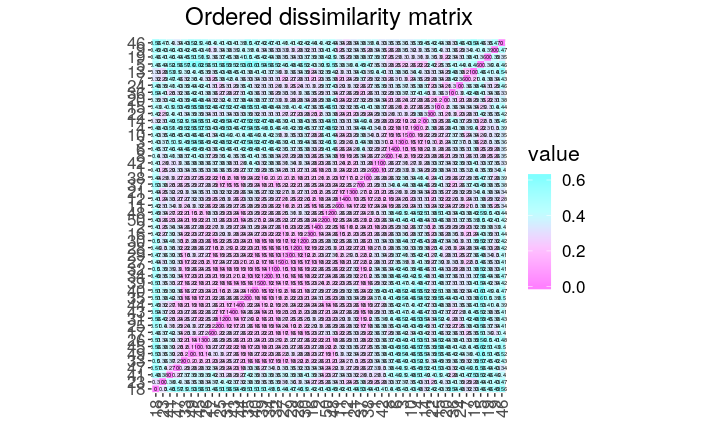
\includegraphics[width=1.00000\textwidth]{matrizdedisimilaridad.png}
\caption{mapa de la isla Barro Colorado matriz disimilaridad
\label{fig:bci_map}}
\end{figure}

\begin{figure}
\centering
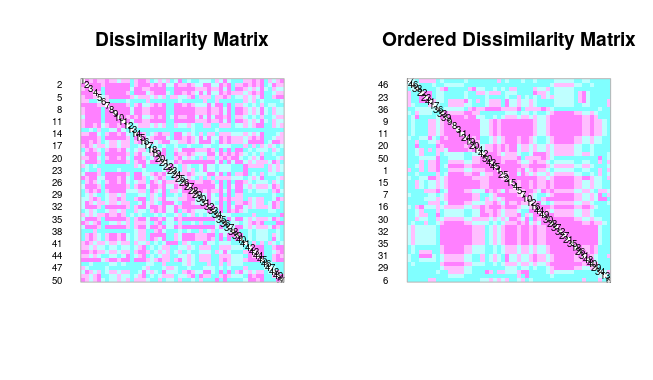
\includegraphics[width=1.00000\textwidth]{matriz_similaridad.png}
\caption{mapa de la isla Barro Colorado matriz disimilaridad
\label{fig:bci_map}}
\end{figure}

\begin{figure}
\centering
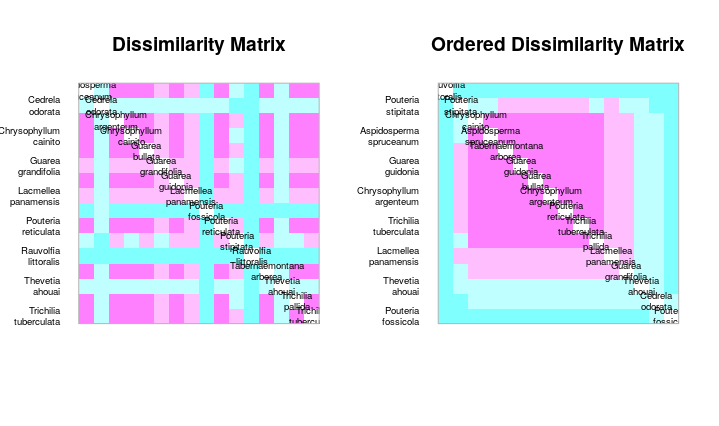
\includegraphics[width=1.00000\textwidth]{mapadecalor.png}
\caption{mapa de la isla Barro Colorado mapa de calor
\label{fig:bci_map}}
\end{figure}

\begin{figure}
\centering
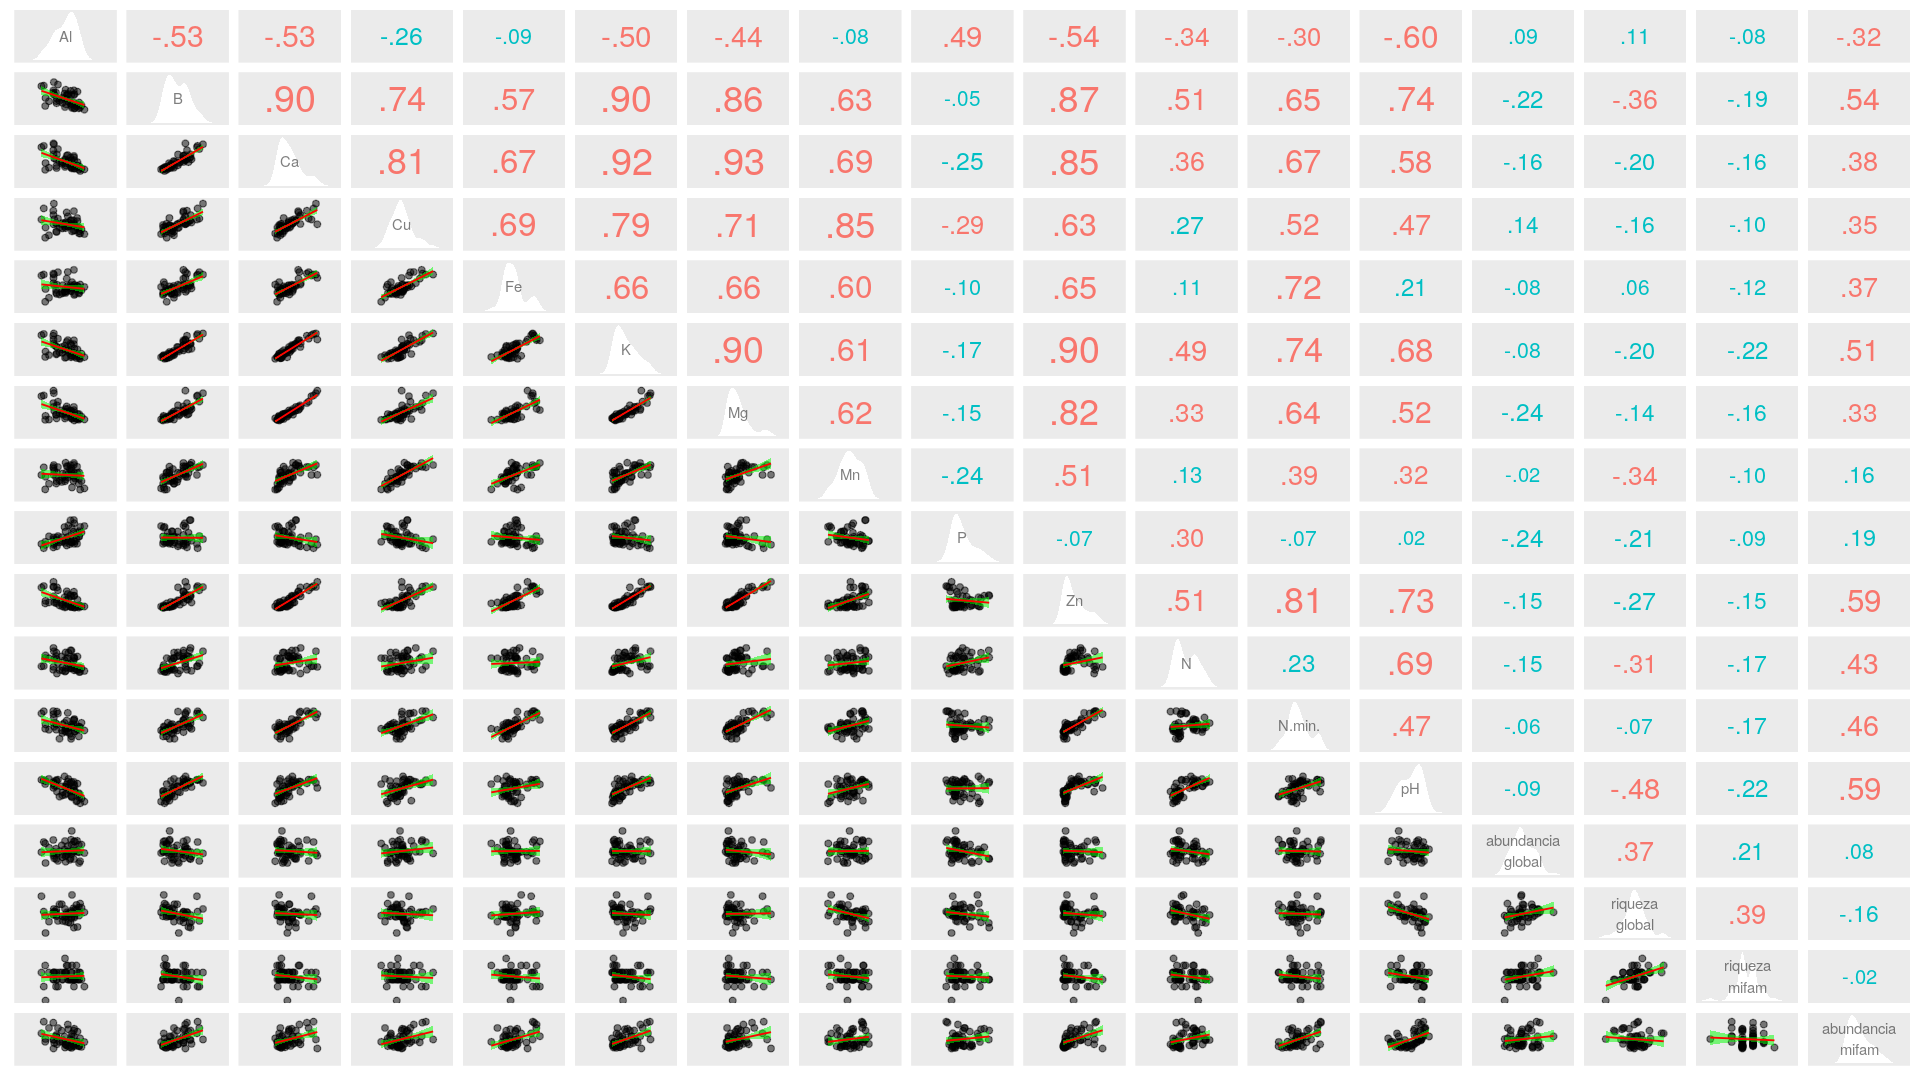
\includegraphics[width=1.00000\textwidth]{matriz_correlacion_suelo_abun_riq_spearman.png}
\caption{mapa de la isla Barro Colorado abundancia y riqueza de suelo
\label{fig:bci_map}}
\end{figure}

\begin{figure}
\centering
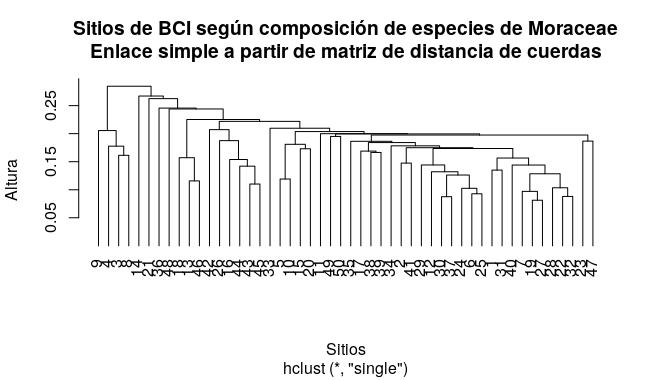
\includegraphics[width=1.00000\textwidth]{sitios_composicion_distancia_cuerdas.png}
\caption{mapa de la isla Barro Colorado sitios de composición por
distancia de cuerda \label{fig:bci_map}}
\end{figure}

\begin{figure}
\centering
\includegraphics[width=1.00000\textwidth]{analisis_interpretacion_dendrogramas.png}
\caption{mapa de la isla Barro Colorado analisis interpretación
dendrogramas \label{fig:bci_map}}
\end{figure}

\begin{figure}
\centering
\includegraphics[width=1.00000\textwidth]{sitios_metodo_ward.png}
\caption{mapa de la isla Barro Colorado sitios de composición por
distancia de cuerda \label{fig:bci_map}}
\end{figure}

\begin{figure}
\centering
\includegraphics[width=1.00000\textwidth]{agrupamiento_dendrograma.png}
\caption{mapa de la isla Barro Colorado sitios de composición por
distancia de cuerda \label{fig:bci_map}}
\end{figure}

\begin{figure}
\centering
\includegraphics[width=1.00000\textwidth]{comparacion_dendrograma_mapa_calor.png}
\caption{mapa de la isla Barro Colorado sitios de composición por
distancia de cuerda \label{fig:bci_map}}
\end{figure}

\begin{figure}
\centering
\includegraphics[width=1.00000\textwidth]{multiescalar_bootstrap.png}
\caption{mapa de la isla Barro Colorado remuestreo multiescalar por
Bootstrap \label{fig:bci_map}}
\end{figure}

\begin{figure}
\centering
\includegraphics[width=1.00000\textwidth]{agrupamiento_dendrogramas_porcentajes.png}
\caption{mapa de la isla Barro Colorado dendrogramas y porcentajes
\label{fig:bci_map}}
\end{figure}

\begin{figure}
\centering
\includegraphics[width=1.00000\textwidth]{mapa_upgma_k2.png}
\caption{mapa de la isla Barro Colorado sitios de composición por
distancia de cuerda \label{fig:bci_map}}
\end{figure}

\begin{figure}
\centering
\includegraphics[width=1.00000\textwidth]{mapas_variables_ambientales.png}
\caption{mapa de la isla Barro Colorado mapa de variables ambientales
\label{fig:bci_map}}
\end{figure}

\begin{figure}
\centering
\includegraphics[width=1.00000\textwidth]{mapa_ward_k3.png}
\caption{mapa de la isla Barro Colorado grupos Ward k3
\label{fig:bci_map}}
\end{figure}

\begin{figure}
\centering
\includegraphics[width=1.00000\textwidth]{cuadro_cajas_ward.png}
\caption{mapa de la isla Barro cuadro de cajas Ward \label{fig:bci_map}}
\end{figure}

\begin{figure}
\centering
\includegraphics[width=1.00000\textwidth]{modelo_abundancia_especie.png}
\caption{mapa de la isla Barro Colorado modelo abundancia de especies
\label{fig:bci_map}}
\end{figure}

\begin{figure}
\centering
\includegraphics[width=1.00000\textwidth]{Numero_individuos.png}
\caption{mapa de la isla Barro Colorado número de individuos
\label{fig:bci_map}}
\end{figure}

\begin{figure}
\centering
\includegraphics[width=1.00000\textwidth]{diversidad_beta.png}
\caption{mapa de la isla Barro Colorado mapa de calor
\label{fig:bci_map}}
\end{figure}

\begin{figure}
\centering
\includegraphics[width=1.00000\textwidth]{mi_fam_hel_pca.png}
\caption{mapa de la isla Barro Colorado diagrama de componentes
principales variables\label{fig:bci_map}}
\end{figure}

\begin{figure}
\centering
\includegraphics[width=1.00000\textwidth]{escalamiento_1_2.png}
\caption{mapa de la isla Barro Colorado diagrama de escalamiento 1 y 2
\label{fig:bci_map}}
\end{figure}

\begin{figure}
\centering
\includegraphics[width=1.00000\textwidth]{rda_escala_especies.png}
\caption{mapa de la isla Barro Colorado RDA diagrama de especies
variables\label{fig:bci_map}}
\end{figure}

\begin{figure}
\centering
\includegraphics[width=1.00000\textwidth]{rda_escalamiento_escala_5.png}
\caption{mapa de la isla Barro Colorado RDA especies no raras
variables\label{fig:bci_map}}
\end{figure}

\begin{figure}
\centering
\includegraphics[width=1.00000\textwidth]{rda_especies_escala_4.png}
\caption{mapa de la isla Barro Colorado RDA digrama de especies
variables\label{fig:bci_map}}
\end{figure}

\includegraphics[width=1.00000\textwidth]{multiples_especies.png} \#
\emph{Script} reproducible

\subsection{Análisis exploratorio de datos. Riqueza y
abundancia}\label{anuxe1lisis-exploratorio-de-datos.-riqueza-y-abundancia}

\begin{verbatim}
#' ---
#' título: 'Análisis exploratorio de datos. Riqueza y abundancia'
#' autor: "JR"
#'fecha: "13 de octubre, 2020"
#' salida: github_document
#' ---

#' ### Área de cargar paquetes
library(vegan)
library(tidyverse)
library(sf)
source('biodata/funciones.R' )

#' ### Área de cargar datos
#' Censo (el objeto se carga con prefijo "censo") y matriz de comunidad (prefijo "mc")
load("~/unidad-0-asignacion-99-mi-manuscrito-GeografosigloXXV/biodata/Moraceae.Rdata")
load('biodata/matriz_ambiental.Rdata') #Matriz ambiental, se carga como "bci_env_grid"

#'### Imprimir datos en pantalla (impresiones parciales con head)
head(censo_morac)
head(mc_morac)
bci_env_grid # No necesita imprimirse parcialment

#' ### También podemos usar
#' Requiere que se haya cargado ya la colección tidyverse
censo_morac %>% tibble
mc_morac %>% tibble

#' ### Lista de especies
sort(colnames(mc_morac))

#' ### Número de sitios, tanto en matriz de comunidad como en ambiental
#' Verifica que coinciden
nrow(mc_morac) #En la matriz de comunidad
nrow(bci_env_grid) #En la matriz ambiental

#' ### Riqueza numérica de especies (usando matriz de comunidad) por quadrat
#'Nota: cargar paquete vegan arriba, en el área de paquetes
specnumber(mc_morac)
sort(specnumber(mc_apcyn_melic_saptc))  # Ordenados ascendentemente
summary(specnumber(mc_morac))  # Resumen estadístico

#' ### Abundancia de especies por quadrat
sort(rowSums(mc_morac))
summary(rowSums(mc_morac))# Resumen estadístico

#' ### Abundancia por especie
sort(colSums(mc_morac))
summary(colSums(mc_morac))# Resumen estadístico

#' ### Riqueza numérica de toda la "comunidad"
specnumber(colSums(mc_morac))

#' ### Abundancia de toda la comunidad
sum(colSums(mc_morac)

#' ### Una tabla para el manuscrito, es necesario asignarle nombre
#' Para esto, usaré la colección "tidyverse"
abun_sp <- (censo_morac) %>%
  group_by(Latin) %>% 
  count() %>% 
  arrange(desc(n))
 abun_sp

#' ### Un gráfico para el manuscrito
#' Gráfico de mosaicos de la abundancia por especie por cuadros
abun_sp_q <- crear_grafico_mosaico_de_mc(mc_apcyn_melic_saptc, tam_rotulo = 6)
abun_sp_q
\end{verbatim}

\subsection{Análisis exploratorio de datos. Mapas de variables
ambientales}\label{anuxe1lisis-exploratorio-de-datos.-mapas-de-variables-ambientales}

\begin{verbatim}
#' ---
#' title: "Análisis exploratorio de datos. Mapas de variables ambientales"
#' author: "JR"
#' date: "25 de octubre, 2020"
#' output: github_document
#' ---

#' ### Cargar paquetes
library(mapview)
library(tidyverse)
library(sf)
library(RColorBrewer)

#' ### Cargar datos
load('biodata/matriz_ambiental.Rdata')

#' ### Paletas
azul <- colorRampPalette(brewer.pal(8, "Blues"))
rojo <- colorRampPalette(brewer.pal(8, "Reds"))
rojo_inv <- colorRampPalette(rev(brewer.pal(8, "Reds")))

#' ### Mapa de cuadros, simbología por pendiente
mapa_cuadros_pendiente <- mapView(
  bci_env_grid,
  layer.name = 'pendiente',
  alpha.regions = 0.4,
  map.types = 'OpenTopoMap',
  legend = T, zoom = 14,
  col.regions = rojo,
  zcol = 'pendiente_media') %>%
  addStaticLabels(label = round(bci_env_grid$pendiente_media, 1)) %>%
  leaflet::setView(
    lng = -79.85136,
    lat = 9.15097,
    zoom = 15)
mapa_cuadros_pendiente
mapa_cuadros_pendiente %>% mapshot(file = 'mapa_cuadros_pendiente.png') #Genera archivo

#' ### Mapa de cuadros, simbología por Nitrógeno
mapa_cuadros_nit <- mapView(
  bci_env_grid,
  layer.name = 'N (mg/kg)',
  alpha.regions = 0.4,
  map.types = 'OpenTopoMap',
  legend = T, zoom = 14,
  col.regions = rojo,
  zcol = 'N') %>%
  addStaticLabels(label = round(bci_env_grid$N, 1)) %>%
  leaflet::setView(
    lng = -79.85136,
    lat = 9.15097,
    zoom = 15)
mapa_cuadros_nit
mapa_cuadros_nit %>% mapshot(file = 'mapa_cuadros_nit.png')

#' ### Mapa de cuadros, simbología por pH
mapa_cuadros_ph <- mapView(
  bci_env_grid,
  layer.name = 'pH',
  alpha.regions = 0.4,
  map.types = 'OpenTopoMap',
  legend = T, zoom = 14,
  col.regions = rojo_inv,
  zcol = 'pH') %>%
  addStaticLabels(label = round(bci_env_grid$pH, 1)) %>%
  leaflet::setView(
    lng = -79.85136,
    lat = 9.15097,
    zoom = 15)
mapa_cuadros_ph
mapa_cuadros_ph %>% mapshot(file = 'mapa_cuadros_ph.png')
\end{verbatim}

\subsection{Análisis de agrupamiento (cluster analysis). Parte 1:
agrupamiento
jerárquico}\label{anuxe1lisis-de-agrupamiento-cluster-analysis.-parte-1-agrupamiento-jeruxe1rquico}

\begin{verbatim}
#' ---
#' title: "Análisis de agrupamiento (cluster analysis). <br> Parte 1: agrupamiento jerárquico"
#' author: "JR"
#' date: "11 de noviembre, 2020"
#' output: github_document
#' ---

knitr::opts_chunk$set(fig.width=12, fig.height=8)

#' ## Preámbulo

#' ### Cargar paquetes
library(vegan)
library(magrittr)
library(broom)
source('biodata/funciones.R')

#' ### Cargar datos
#' 
load('biodata/Moraceae.Rdata')
mi_fam <- mc_morac
#'
#' ## Características de las técnicas de agrupamiento
#' 
#' Las técnicas de agrupamiento se clasifican según los algoritmos que emplean y el orden de ejecución, así como según el tipo de enfoque inferencial. Los algoritmos de agrupamiento pueden ser:
#' 
#' - Secuenciales o simultáneos.
#' - Por aglomeración o por división. En referencias en español encontrarás "aglomerativos" y "divisivos", pero ten presente que la primera grafía no está en el Diccionario.
#' - Monotéticos o politéticos.
#' - Jerárquicos o no jerárquicos.
#' - Probabilísticos o no probabilísticos.
#' - Restringidos o no restringidos.
#' 
#' ## Agrupamiento jerárquico
#' 
#' El agrupamiento jerárquico (AJ) es una técnica de agrupamiento secuencial que consiste en la repetición de un procedimiento dado para agrupar objetos hasta que todos encuentran un lugar. **Los resultados del AJ comúnmente se muestran en dendrogramas**.
#' 
#' Dentro del AJ es frecuente usar un enfoque aglomerativo, lo cual implica aplicar algoritmos secuenciales desde abajo hacia arriba. Bajo este enfoque, se comienza con una colección discontinua de objetos que son subsecuentemente agrupados en grupos (clusters) cada vez más grandes, hasta alcanzar un único grupo que engloba a todos los subgrupos.
#' 
#' El AJ aglomerativo dispone de varios algoritmos de resolución del agrupamiento por pares, que son los denominados **"criterios de enlace"**. Los más usados son: "de enlace simple", "de enlace completo" y "de enlace promedio".
#' 
#' Normalmente, en el análisis de agrupamiento nos interesa agrupar sitios en función de sus descriptores que, en una matriz de comunidad, son sus especies, y en una matriz ambiental son las variables que caracterizan los microhábitats. En mi caso y en el de ustedes, los sitios son los 50 cuadros de 1 Ha (quadrats); el resultado de este primer script serán dendrogramas con los que podremos explorar, de manera visual y analítica, cuántos grupos hacen sentido y, con suerte, determinar a qué grupo parece pertenecer cada sitio (siguiente script).
#' 
#' Dado que los cuadros en BCI están autocorrelacionados espacialmente, violamos el supuesto de independencia de las observaciones. Esto limita el alcance de nuestros resultados, pero no los invalida, y al mismo tiempo nos ofrecen una oportunidad estupenda para evaluar las técnicas mostradas a continuación.
#' 
#' ### Agrupamiento "aglomerativo" por enlace simple
#' 
#' Este método utiliza, como criterio de enlace para agrupar sucesivamente pares de objetos, la mayor similaridad ("mínima distancia" o "vecino más próximo"). Comúnmente, los dendrogramas muestran un encadenamiento de objetos, a modo de escaleras.
#' 
#' Para aplicar este método, debes transformar la matriz de comunidad utilizando alguno de los métodos explicados en medición de la asociación. En este caso, utilizaré el método de normalización y luego obtendré la distancia euclidea (distancia de cuerdas o *chord*).
#' 
mi_fam_norm <- decostand(mi_fam, "normalize")
mi_fam_norm_d <- vegdist(mi_fam_norm, "euc")
mi_fam_norm_d %>% tidy
#'
#' Es importante, para garantizar consistencia a lo largo del agrupamiento, asignar los nombres de sitios al atributo `labels` del objeto de distancias.
#' 
attr(mi_fam_norm_d, "labels") <- rownames(mi_fam)
#' 
#' Posteriormente, el agrupamiento jerárquico lo realizaré con la función `hclust` del paquete `stats` (se carga por defecto al abrir R), especificando el argumento `method = 'single'`:
#' 
(cl_single <- hclust(mi_fam_norm_d, method = 'single'))
#' 
#' Finalmente, el dendrograma a continuación:
plot(cl_single, labels = rownames(mi_fam), hang = -1,
     main = "Sitios de BCI según composición de especies de Moraceae\nEnlace simple a partir de matriz de distancia de cuerdas",
     xlab = 'Sitios', ylab = 'Altura')
#' 
#' ### Agrupamiento "aglomerativo" por enlace completo
#' 
#' En este caso, el criterio de enlace para agrupar sucesivamente pares de objetos es la menor similaridad ("máxima distancia" o "vecino más lejano"). Crearé el dendrograma a partir de la misma matriz de distancia de cuerdas empleada en el dendrograma anterior.
#' 
(cl_complete <- hclust(mi_fam_norm_d, method = 'complete'))
plot(cl_complete, labels = rownames(mi_fam), hang = -1,
     main = "Sitios de BCI según composición de especies de Moraceae\nEnlace completo a partir de matriz de distancia de cuerdas",
     xlab = 'Sitios', ylab = 'Altura')
#' 
#' ### Agrupamiento "aglomerativo" por enlace promedio
#' 
#' En este caso, el criterio de enlace para agrupar sucesivamente pares de objetos es el promedio entre grupos, el cual a su vez puede ser de dos tipos: media o centroide. Este método es más bien una familia de submétodos, clasificados en función del tipo de promedio empleado y el peso asignado a las distancias originales (número de elementos de los clusters que se agrupan progresivamente).
#' 
#' Así, dependiendo de si se media o centroide, o si se ponderan o no las distancias originales, se producen cuatro combinaciones de submétodos: grupos de pares no ponderados con media aritmética (unweighted pair-group method using arithmetic averages, UPGMA), grupos de pares ponderados con media aritmética (WPGMA), grupos de pares no ponderados con centroide (UPGMC) y grupos de pares ponderados con centroide (WPGMC). El más usado es UPGMA, porque máximiza la correlación entre la distancia cofenética (ver siguiente script) y la matriz de distancia original.
#' 
#' Sólo crearé el dendrograma del método UPGMA.
#' 
(cl_upgma <- hclust(mi_fam_norm_d, method = 'average'))
plot(cl_upgma, labels = rownames(mi_fam), hang = -1,
     main = "Sitios de BCI según composición de especies de Moraceae\nUPGMA a partir de matriz de distancia de cuerdas",
     xlab = 'Sitios', ylab = 'Altura')
#' 
#' ### Agrupamiento por el método de Ward de varianza mínima
#' 
#' Se basa en los mismos supuestos y criterios de la regresión lineal por mínimos cuadrados, similar a lo establecido para el ANOVA, que a fin de cuentas es un caso particular de regresión lineal. El objetivo es definir grupos de manera que la suma de cuadrados se minimice dentro de cada uno de ellos.
#' 
(cl_ward <- hclust(mi_fam_norm_d, method = 'ward.D2'))
plot(cl_ward, labels = rownames(mi_fam), hang = -1,
     main = "Sitios de BCI según composición de especies de Moraceae\nMétodo de Ward a partir de matriz de distancia de cuerdas",
     xlab = 'Sitios', ylab = 'Altura')
\end{verbatim}

\subsection{Análisis de agrupamiento (cluster analysis). Parte 2:
Interpretación y comparación de
resultados}\label{anuxe1lisis-de-agrupamiento-cluster-analysis.-parte-2-interpretaciuxf3n-y-comparaciuxf3n-de-resultados}

\begin{verbatim}
#' ---
#' title: "Análisis de agrupamiento (cluster analysis). <br> Parte 2: Interpretación y comparación de resultados"
#' author: "JR"
#' date: "11 de noviembre, 2020"
#' output: github_document
#' ---

knitr::opts_chunk$set(fig.width=12, fig.height=8)

#' ## Preámbulo
#' 
#' ### Cargar paquetes
#' 
library(vegan)
library(tidyverse)
library(broom)
library(cluster)
library(gclus)
library(pvclust)
library(sf)
source('biodata/funciones.R')
#' 
#' ### Cargar datos
#' 
load('biodata/Moraceae.Rdata')
mi_fam <- mc_morac
load('biodata/matriz_ambiental.Rdata')
mi_fam %>% tibble
bci_env_grid %>% tibble
#' 
#' ### Generar matriz de distancias de cuerdas
#' 
mi_fam_norm <- decostand(mi_fam, "normalize")
mi_fam_norm_d <- vegdist(mi_fam_norm, "euc")
mi_fam_norm_d %>% tidy
#' 
#' ## Interpretación visual de dendrogramas
#' 
#' [En el script anterior](aa_analisis_de_agrupamiento_1_jerarquico.md) realicé los dendrogramas a partir de una matriz de cuerdas aplicando distintos métodos. El objetivo de este script es mostrarte cómo explorar, de manera visual y analítica, cuál o cuáles métodos de agrupamiento son idóneos para sintetizar tus resultados, cuántos grupos hacen sentido en un análisis de agrupamiento y, con suerte, determinar a qué grupo parece pertenecer cada sitio.
#' 
#' La primera evaluación de los dendrogramas NO debe venir de la mano de sofisticados análisis ni de procedimientos mecánicos. Te recomiendo que los explores visualmente, con la intención de identificar grupos (clústers) consistentes, es decir, aquellos que se repiten entre dendrogramas. Asimismo, identifica aquellos elementos que, de manera consistente entre dendrogramas, no parezcan agruparse con otros.
#' 
#' Evita concentrar tu vista en grupos extremadamente pequeños; comienza analizando el árbol desde arriba hacia abajo, prefiere encontrar grupos grandes y consistentes entre dendrogramas (si los hay). No atomices el dendrograma a menos que sea estrictamente necesario. Observar muchos grupos pequeños te impedirá ver los posibles patrones globales. Ahora bien, si hubiere grupos pequeños reiteradamente, entonces considéralos. No obstante, los cuadros de 1 Ha de la parcela de BCI están autocorrelacionados espacialmente, por lo que normalmente encontrarás grupos grandes.
#' 
#' Anota tus impresiones, para que las compares con los resultados que posteriormente obtendrás; si confirmas patrones detectados visualmente, la evidencia se irá acumulando en una dirección. Si por el contrario, detectas inconsistencia, es el momento de revisar los scripts de generación de dendrogramas; si luego de revisar ves que todo está correcto, entonces debes seguir explorando patrones con otras técnicas o utilizando distintos criterios de agrupamiento. Cuando termines la exploración visual, entonces continúa aplicando otras técnicas analíticas.
#'
#' Para la exploración visual, generaré los objetos de cluster dentro de una lista:
#' 
lista_cl <- list(
  cl_single = hclust(mi_fam_norm_d, method = 'single'),
  cl_complete = hclust(mi_fam_norm_d, method = 'complete'),
  cl_upgma = hclust(mi_fam_norm_d, method = 'average'),
  cl_ward = hclust(mi_fam_norm_d, method = 'ward.D2')
)
#' 
#' Un plot en panel 2x2 ayuda a visualizarlos todos de manera conjunta. En tu caso, observa y compara todos los dendrogramas:
#' 
par(mfrow = c(2,2))
invisible(map(names(lista_cl), function(x) plot(lista_cl[[x]], main = x, hang = -1)))
par(mfrow = c(1,1))
#' 
#' En mi caso, exceptuando el dendrograma generado por medio del enlace simple, detecto al menos 2 grupos consistentes (integrados por múltiples posibles subgrupos), los cuales mencionaré usando los identificadores de sitios:
#' 
#' - Un grupo pequeño, compuesto por los sitios 1, 42, 12, 21, 11, 2 y 16.
#' - Un "grupo" heterogéneo y grande, conformado por 25, 31,..., 26,..., 35,..., 34,...,32, 17,..., 30, que también parece incluir a 44, 49, 47, 48, 50.
#' 
#' Además de los grupos anteriores, detecto elementos que no forman grupos, es decir, sitios que aparecen aislados del resto, como por ejemplo el 46 y, en algunos métodos, también el 9.
#' 
#' ## Elegir método y número de clústers
#' 
#' Existen varios criterios para elegir un dendrograma idóneo, como por ejemplo, los gráficos tipo-Shepard y la correlación cofenética. Centraré mi atención en esta última. Igualmente, una vez elijas el método de agrupamiento idóneo, existen varios métodos para decidir cuántos clústers son óptimos, como la anchura de silueta (*silhouette width*, que explicaré) y los niveles de fusión (*fusion levels*, este último te lo dejo para autoapredizaje).
#' 
#' ### Seleccionar método de agrupamiento por correlación cofenética
#' 
#' La correlación cofenética impica conocer la distancia cofenética, y esta última se entiende mejor con un ejemplo: elige un objeto (e.g. sitio, cuadro de 1 ha) cualquiera, "escala" por el árbol hasta llegar a un nodo, luego desciende hasta el objeto más cercano. El recorrido que acabas de realizar se denomina distancia cofenética. Ahora, hipotéticamente, construye una matriz de distancias cofenéticas entre todos los objetos (a pares), y calcula la correlación de ésta con la matriz de distancias original. Esto último se denomina "correlación cofenética". El método con el valor más alto de correlación cofenética es el que mejor sintetiza la distancia original y, por lo tanto, será el preferido. Normalmente, la mayor correlación cofenética la brindan UPGMA y enlace completo, pero no elijas un método de agrupamiento mecánicamente basándote sólo en este criterio (ver notas más adelante al respecto).
#' 
#' Usando la lista de objetos de clústers, calcularé la correlación cofenética dentro de un `map` (una función del paquete `purrr`, perteneciente a la colección `tidyverse`), para así repetir el mismo proceso con los cuatro objetos de clusters en una sentencia:
#'
map_df(lista_cl, function(x) {
  coph_d <- cophenetic(x)
  corr <- cor(mi_fam_norm_d, coph_d)
  return(corr)
})
#' 
#' Habrás notado que, tanto UPGMA como enlace completo, tienen valores altos de correlación cofenética. Un método complementario para explorar la correlación cofenética es el diagrama tipo-Shepard, el cual te recomiendo aprender a usar por tu cuenta si deseas profundizar.
#' 
#' ### Elegir número de clústers
#' 
#' Elegiré UPGMA como método de agrupamiento y determinaré cuántos grupos son idóneos de acuerdo a su anchura de silueta (*silhouette width*). Sin embargo, no lo haré sólo para UPGMA, también contrastaré con Ward. ¿Por qué? De entrada, se sabe que UPGMA tendrá una buena correlación cofenética, dado que dicho método está diseñado para maximizarla. Sin embargo, me interesa explorar patrones con sentido ecológico, no sólo seguir procedimientos mecánicos y, al menos en mi caso, el método de Ward podría hacer más sentido ecológico que UPGMA.
#' 
#' El objetivo de la función `calcular_anchuras_siluetas` está implícito en su nombre, y requiere de tres argumentos: matriz de comunidad original, matriz de distancias, y objeto de clúster. Devuelve como resultado una lista con dos objetos (los explico más abajo):
#' 
#' 1. Las anchuras promedio para cada partición, excepto para las particiones `i=1` y `i=50`, por ser irrelevantes (se les asigna 0);
#' 
#' 2. Número óptimo de grupos. Haré los cálculos para UPGMA y Ward, y luego explico en qué consisten los resultados.
#' 
#' Para UPGMA:
#' 
anch_sil_upgma <- calcular_anchuras_siluetas(
  mc_orig = mi_fam, 
  distancias = mi_fam_norm_d, 
  cluster = lista_cl$cl_upgma)
anch_sil_upgma
#' 
#' El objeto `anchuras_siluetas` de la lista `anch_sil_upgma` te muestra un vector con los promedios de anchuras de siluetas para todas las posibles particiones con sentido. Al ser promedios, lo que reflejan es el valor de las siluetas de manera general. Si para una partición dada, se registran promedios de siluetas grandes, se interpreta entonces que habrá muchos casos de grupos claramente aislados para dicha partición.
#' 
#' Igualmente, el objeto `n_grupos_optimo` te indica cuál es el número óptimo de clústers a crear, es decir, en cuántos grupos cortar el árbol. Esto se determina programáticamente por medio de la posición que ocupa el promedio más alto, que en este caso es la posición dos. Sin embargo, te recomiendo NO usar este número a ciegas. Verifica si el valor máximo, que en este caso ocupa la posición dos, se diferencia o se parece mucho a los de su entorno, por ejemplo, al valor de la posición 3. En mi caso, el valor de anchura promedio de la posición 2 se diferencia, por mucho, del de la posición 3. Por lo tanto, puedo elegir con seguridad 2 como número de clústers óptimo.
#' 
#' Haré el gráfico de dendrograma, aunque nota que en este caso primero reordenaré los sitios con la función `reorder.hclust`, de tal suerte que los sitios más próximos en términos de distancias aparecerán próximos también en el dendrograma.
#' 
u_dend_reord <- reorder.hclust(lista_cl$cl_upgma, mi_fam_norm_d)
plot(u_dend_reord, hang = -1)
rect.hclust(
  tree = u_dend_reord,
  k = anch_sil_upgma$n_grupos_optimo)
#' 
#' Ahora compararé el dendrograma con el mapa de calor en un mismo gráfico, colocando los dendrogramas en los márgenes del gráfico. Verificaré si el número de grupos hace sentido, recordando los grupos que inicialmente identifiqué.
#' 
heatmap(
  as.matrix(mi_fam_norm_d),
  Rowv = as.dendrogram(u_dend_reord),
  symm = TRUE,
  margin = c(3, 3),
  col = rev(cm.colors(4))
)
#' 
#' En general, hay dos grupos, uno grande y otro pequeño, y parece haber un tercero en el mapa de calor. El grupo grande ocupa la mancha rosa central que se extiende hasta el borde inferior derecho, y el grupo pequeño ocupa la posición superior derecha. Aunque los promedios de anchura de siluetas sugerían usar 2 grupos, el mapa de calor parece sugerir que existe un tercer grupo entre los dos anteriores, representado por los sitios 18, 8,..., 7,..., 19.
#' 
#' Mostraré el resultado para Ward:
#' 
anch_sil_ward <- calcular_anchuras_siluetas(
  mc_orig = mi_fam, 
  distancias = mi_fam_norm_d, 
  cluster = lista_cl$cl_ward)
anch_sil_ward
#' 
#' En este caso, el valor máximo, que ocupa la posición número 2, no se diferencia mucho del de la posición 3. Al parecer, sería igualmente válido elegir 2 o 3 particiones, por tener promedios de anchuras de siluetas bastante parecidos. Por tal razón, cortaré el dendrograma en 2 y en 3 grupos, respectivamente:
#' 
w_dend_reord <- reorder.hclust(lista_cl$cl_ward, mi_fam_norm_d)
plot(w_dend_reord, hang = -1)
rect.hclust(
  tree = w_dend_reord,
  k = anch_sil_ward$n_grupos_optimo)
plot(w_dend_reord, hang = -1)
rect.hclust(
  tree = w_dend_reord,
  k = anch_sil_ward$n_grupos_optimo + 1)
#' 
#' Comparando el dendrograma con el mapa de calor. Verificar si el número de grupos hace sentido.
#' 
heatmap(
  as.matrix(mi_fam_norm_d),
  Rowv = as.dendrogram(w_dend_reord),
  symm = TRUE,
  margin = c(3, 3),
  col = rev(cm.colors(4))
)
#' 
#' Nótese que este dendrograma hace más sentido que el sugerido por UPGMA. En cualquier casos, conservaré ambos resultados para seguir evaluando a posteriori y contrastando con nuevos métodos.
#' 
#' ### Evaluación mediante remuestreo por *bootstrap* multiescalar
#' 
#' Con suerte, un agrupamiento aplicado a datos muestrales reflejará los patrones naturales de organización. Sin embargo, lo que con toda seguridad mostrará es el sesgo de muestreo. Afortunadamente, los datos de BCI son censales, por lo que el sesgo de muestreo es una preocupación menor o inexistente.
#' 
#' Sin embargo, los datos de BCI también tienen sesgo, pues se usa un DAP de corte para decidir si un individuo es censado o no. Si consideramos que el universo es "todos los individuos de 1 cm o más de tallo", pues el sesgo es bajísimo, pero si quisiéramos extraer conclusiones aplicadas a toda comunidad, cometeríamos errores debidos a sesgo por muestreo.
#' 
#' No obstante, aun con todas sus bondades, los datos censales carecen de una fortaleza: no reflejan asociación con grandes unidades de hábitats y, a lo sumo, revelan asociación con microhábitats muy específicos, por lo que extraer conclusiones sobre patrones de asociación con variables ambientales de manera más general, presenta sus limitaciones.
#' 
#' Por estas razones, los análisis de agrupamientos realizados hasta este punto, reflejan tanto el mencionado sesgo y las limitaciones impuestas por el pequeño espacio territorial estudiado. Una forma de validar la robustez de los resultados anteriores, consiste en realizar un remuestreo por medio de *bootstrap*, un método que consiste en tomar muestras aleatorias de los datos y realizar, con cada una, análisis de agrupamiento. Este proceso se repite varias veces (e.g. 1000 veces), es decir, se realizan varias iteraciones. Al finalizar, se cuenta la proporción de veces que un grupo dado aparece consistentemente como clúster (tasa de éxito), la cual se denomina probabilidad de *bootstrap* del clúster en cuestión (*bootstrap probability*, BP). A este procedimiento se le ha añadido más recientemente el criterio de remuestreo por *bootstrap* multiescalar, es decir, considerar muestras de tamaños diferentes, a lo que se denomina valores de probabilidad aproximadamente insesgados (*approximately unbiased*, AU). Los valores de AU son, en principio, más fiables que los de BP, por lo que serán los preferidos en este análisis.
#' 
#' El método de remuestreo por *boostrap* multiescalar está implementado en el paquete `pvclust`, y la función del mismo nombre se encarga de realizarlo. IMPORTANTE: la matriz de comunidad, que en este caso es la matriz normalizada, debe transponerse previamente; de ahí que verás el uso de la función `t()` en el primer argumento de `pvclust`. La función primero genera un agrupamiento, por lo que debemos especificar con qué método, en este caso lo haré tanto con UPGMA como con Ward, para así validar los dos métodos ejecutados anteriormente.
#' 
#' La función `pvclust` devolverá un dendrograma enriquecido, que incluirá los valors de AU y BP de cada nodo del dendrograma en cuestión. Los valores de AU serán especialmente relevantes, porque con ellos trazaré dos "decoraciones" de ayuda:
#' 
#' - Rectángulos de borde azul, para todos aquellos grupos que resulten con valores de AU>0.91 en sus nodos. Estos rectángulos permitirán ver los grandes grupos sin perder robustez, dado que prefiero el enfoque de agrupador (*lumper*) por encima del desglosador (*splitter*); con esto además evito la tendencia de dividir en demasiados grupos pequeños, la cual vengo evitando desde análisis anteriores por el alto grado de autocorrelación espacial que afecta a los datos de BCI.
#' 
#' - Líneas inferiores rojas, que resaltan aquellos grupos (o subgrupos) que obtuvieron AU>0.95. Estos grupos son considerados como sólidamente coherentes, es decir, aquellos cuya singularidad es prácticamente indiscutible. No obstante, suelen ser pequeños con relación a los anteriores.
#' 
#' Ten presente que, al realizar remuestreo por *bootstrap* multiescalar, cada corrida puede arrojar resultados diferentes, dado que el procedimiento implica remuestreo. No obstante, los patrones indiscutibles estarán siempre presentes en cada corrida. Para garantizar reproducibilidad, utilicé el argumento `iseed` en la función `pvclust`.
#' 
#' #### UPGMA
#' 
cl_pvclust_upgma <-
  pvclust(t(mi_fam_norm),
          method.hclust = "average",
          method.dist = "euc",
          iseed = 91, # Resultado reproducible
          parallel = TRUE)
# Añadir los valores de p
plot(cl_pvclust_upgma, hang = -1)
# Añadir rectángulos a los grupos significativos
lines(cl_pvclust_upgma)
pvrect(cl_pvclust_upgma, alpha = 0.91, border = 4)
#' 
#' #### Ward
#' 
cl_pvclust_ward <-
  pvclust(t(mi_fam_norm),
          method.hclust = "ward.D2",
          method.dist = "euc",
          iseed = 191, # Resultado reproducible
          parallel = TRUE)
# Añadir los valores de p
plot(cl_pvclust_ward, hang = -1)
# Añadir rectángulos a los grupos significativos
lines(cl_pvclust_ward)
pvrect(cl_pvclust_ward, alpha = 0.91, border = 4)
#' 
#' ### Recapitulando los grupos de sitios.
#' 
#' #### Patrones comunes y dispares
#' 
#' Detecto algunos patrones consistentes en cuanto a grupos de sitios según composición de las especies de mi familia asignada:
#' 
#' - Tanto en UPGMA como en Ward, detecté al menos dos o tres grandes grupos. Con el primer método, UPGMA, noté buena coincidencia entre el número de grupos detectados por el criterio de *silhouette width* y por `pvclust`.
#' 
#' - En el caso específico del dendrograma Ward, `pvclust` atomizó los sitios en demasiados grupos. Este resultado podría ser de interés para determinados análisis, como por ejemplo, si se consideraran microhábitats muy específicos o si entre mis familia asignada se registrasen especialistas muy selectivos.
#' 
#' #### ¿Cómo declaro los grupos de sitios?
#' 
#' Para conservar las clasificaciones de grupos de sitios anteriores, crearé un vector con el identificador del grupo al que pertenece cada grupo. Es importante imprimir el resultado, para confirmar que los sitios estén ordenados según aparecen en las matrices de comunidad y ambiental.
#' 
#' UPGMA:
(grupos_upgma_k2 <- as.factor(cutree(lista_cl$cl_upgma, k = 2)))
#' 
#' En este caso, los sitios 1 y 2 pertenecen al grupo 1, los sitios 3 al 6 pertenecen al grupo 2, nuevamente, del 7 al 9 pertenecen al grupo 1, el sitio 10 pertenece al grupo 2, y así sucesivamente. Preguntaré cuántos sitios hay en cada grupo mediante la función `table`:
#' 
table(grupos_upgma_k2)
#' 
#' Nota lo desiguales que son estos grupos, un efecto esperado dado el alto grado de autocorrelación espacial que tienen entre sí los cuadros de 1 Ha de BCI. Este desequilibrio afecta las inferencias que realizaré en *scripts* posteriores, pero para fines didácticos los realizaré de todas maneras. No obstante, en tu caso, esperaría y desearía que tu familia asignada ofrezca resultados de agrupamiento más equilibrados.
#' 
#' Ward:
#' 
(grupos_ward_k3 <- as.factor(cutree(lista_cl$cl_ward, k = 3)))
table(grupos_ward_k3)
#'
#' Guardaré estos vectores en archivos para reutilizarlos en *scripts* posteriores:
#' 
saveRDS(grupos_upgma_k2, 'grupos_upgma_k2.RDS')
saveRDS(grupos_ward_k3, 'grupos_ward_k3.RDS')
#' 
#' Evita usar este, y cualquier otro procedimiento, de manera mecánica. En tu caso, quizá tengas que cortar tus dendrogramas en más o menos grupos de sitios. También podría resultar que alguno de dichos métodos, o ambos, sean irrelevante para tu caso, por lo que probablemente tendrás que elegir otro que haga sentido ecológico a tus datos (por ejemplo, *complete*).
#' 
#' En el próximo *script*, aprenderás a comparar este resultado con las variables ambientales. También podrás evaluar cómo se distribuyen los grupos de sitios en un mapa, usando las herramientas del paquete `mapview`.
\end{verbatim}

\subsection{Análisis de agrupamiento (cluster analysis). Parte 3: Grupos
(clústers), variables ambientales y
mapas}\label{anuxe1lisis-de-agrupamiento-cluster-analysis.-parte-3-grupos-cluxfasters-variables-ambientales-y-mapas}

\begin{verbatim}
#' ---
#' title: "Análisis de agrupamiento (cluster analysis). <br> Parte 3: Grupos (clústers), variables ambientales y mapas"
#' author: "JR"
#' date: "15 de noviembre, 2020"
#' output: github_document
#' ---

knitr::opts_chunk$set(fig.width=12, fig.height=8)

#' ## Preámbulo
#' 
#' ### Cargar paquetes
#' 
library(mapview)
library(tidyverse)
library(sf)
library(RColorBrewer)
source('biodata/funciones.R')
#' 
#' ### Cargar datos
#' 
load("~/unidad-0-asignacion-99-mi-manuscrito-GeografosigloXXV/biodata/Moraceae.Rdata")
load('biodata/matriz_ambiental.Rdata')
grupos_upgma_k2 <- readRDS('grupos_upgma_k2.RDS')
table(grupos_upgma_k2) #Importante, tener en cuenta los desiguales tamaños de los grupos
grupos_ward_k3 <- readRDS('grupos_ward_k3.RDS')
table(grupos_ward_k3)
#' 
#' ### Paletas
#' 
rojo <- colorRampPalette(brewer.pal(8, "Reds"))
rojo_inv <- colorRampPalette(rev(brewer.pal(8, "Reds")))
colores_grupos <- brewer.pal(8, "Accent")
#' 
#' ## Explorar efectos
#' 
#' ### Pruebas de igualdad de promedios de las variables entre 2 grupos
#' 
#' Para evaluar homogeneidad de promedios usaré las pruebas *t* (medias), basada en la distribución *t* de *Student*, y la prueba no paramétrica de la suma de rangos de Wilcoxon (medianas), usando como variable de agrupamiento los grupos establecidos en el agrupamiento UPGMA. Nota que en mi caso UPGMA clasifica los sitios en dos grupos, pero en tu caso podría ser distinto (para evaluar homogeneidad de promedios de un número mayor de grupos, ver sección siguiente).
#' 
#' Primero crearé un objeto que permita realizar tanto las pruebas como los diagramas de cajas.
#' 
(m_amb_upgma_k2 <- bci_env_grid %>%
    select_if(is.numeric) %>% select(-id) %>% 
    mutate(grupos_upgma_k2) %>%
    st_drop_geometry() %>% 
    pivot_longer(-grupos_upgma_k2, names_to = "variable", values_to = "valor"))
#' 
#' A continuación, las pruebas:
#' 
m_amb_upgma_k2 %>%
  group_by(variable) %>%
  summarise(
    p_valor_t = t.test(valor ~ grupos_upgma_k2)$p.value,
    p_valor_w = wilcox.test(valor ~ grupos_upgma_k2, exact = F)$p.value) %>%
  arrange(p_valor_t) %>%
  print(n=Inf)
#' 
#' Interesa observar las variables que obtuvieron valores de p<0.01. Reitero que, en mi caso, mis grupos resultaron muy desiguales, recordando: el grupo 1 tiene 43 sitios (43) y el grupo 2 tiene 7. Este desigual número de sitios por grupo, hace que la prueba estadística pierda potencia, porque se viola la recomendación de evitar tamaños de los tratamientos muy desiguales.
#' 
#' Por otra parte, este es un buen momento para "revisitar" tus análisis exploratorios de datos (AED), específicamente el análisis de correlación (*script* 5). Es probable que algunas de las variables ambientales que presentaron efecto entre grupos (las que obtuvieron p<0.01), te aparezca también como significativamente correlacionada con la abundancia o la riqueza en el script 5 de AED.
#' 
#' Los gráficos:
#' 
m_amb_upgma_k2 %>% 
  group_by(variable) %>% 
  ggplot() + aes(x = grupos_upgma_k2, y = valor, fill = grupos_upgma_k2) + 
  geom_boxplot() + 
  scale_fill_brewer(palette = 'Accent') +
  theme_bw() +
  theme(legend.position="none") +
  facet_wrap(~ variable, scales = 'free_y')
#' 
#' Mapas:
#' 
mapa_upgma_k2 <- mapView(
  bci_env_grid %>% mutate(grupos_upgma_k2),
  layer.name = 'Grupos (2) UPGMA',
  alpha.regions = 0.6,
  map.types = 'OpenTopoMap',
  legend = T,
  col.regions = colores_grupos[1:2],
  zcol = 'grupos_upgma_k2') %>%
  addStaticLabels(label = bci_env_grid$id) %>% 
  leaflet::setView(
    lng = -79.85136,
    lat = 9.15097,
    zoom = 15)
mapa_upgma_k2
mapa_upgma_k2 %>% mapshot(
  file = 'mapa_upgma_k2.png', 
  remove_controls = c("zoomControl", "layersControl", "homeButton")
)
#' 
#' Mapa de una de las variables donde se presentó efecto de su promedio (p<0.01), en este caso, Zinc (`Zn`)
#' 
mapa_zn <- mapView(
  bci_env_grid,
  layer.name = 'Zinc',
  alpha.regions = 0.6,
  map.types = 'OpenTopoMap',
  legend = T,
  col.regions = rojo,
  zcol = 'Zn') %>%
  addStaticLabels(label = bci_env_grid$id) %>% 
  leaflet::setView(
    lng = -79.85136,
    lat = 9.15097,
    zoom = 15)
mapa_zn
mapa_zn %>% mapshot(
  file = 'mapa_zinc.png', 
  remove_controls = c("zoomControl", "layersControl", "homeButton")
)
#' 
#' ### Pruebas de igualdad de promedios de las variables entre 3 grupos o más
#' 
#' Objeto común:
#' 
(m_amb_ward_k3 <- bci_env_grid %>%
    select_if(is.numeric) %>% select(-id) %>% 
    mutate(grupos_ward_k3) %>%
    st_drop_geometry() %>% 
    pivot_longer(-grupos_ward_k3, names_to = "variable", values_to = "valor"))
#' 
#' Pruebas, en este caso ANOVA (evalúa homogeneidad de medias; no se cumplen muchos de los supuestos requeridos para esta prueba) y Kruskal-Wallis (evalúa homogeneidad de medianas):
#' 
m_amb_ward_k3 %>% 
  group_by(variable) %>% 
  summarise(
    p_valor_a = oneway.test(valor ~ grupos_ward_k3)$p.value,
    p_valor_k = kruskal.test(valor ~ grupos_ward_k3)$p.value) %>%
  arrange(p_valor_k) %>%
  print(n=Inf)
#' 
#' Gráficos:
#' 
m_amb_ward_k3 %>% 
  group_by(variable) %>% 
  ggplot() + aes(x = grupos_ward_k3, y = valor, fill = grupos_ward_k3) + 
  geom_boxplot() + 
  scale_fill_brewer(palette = 'Accent') +
  theme_bw() +
  theme(legend.position="none") +
  facet_wrap(~ variable, scales = 'free_y')
#' 
#' Mapas:
#' 
mapa_ward_k3 <- mapView(
  bci_env_grid %>% mutate(grupos_ward_k3),
  layer.name = 'Grupos (3) Ward',
  alpha.regions = 0.6,
  map.types = 'OpenTopoMap',
  legend = T,
  col.regions = colores_grupos[1:3],
  zcol = 'grupos_ward_k3') %>%
  addStaticLabels(label = bci_env_grid$id) %>% 
  leaflet::setView(
    lng = -79.85136,
    lat = 9.15097,
    zoom = 15)
mapa_ward_k3
mapa_ward_k3 %>% mapshot(
  file = 'mapa_ward_k3.png', 
  remove_controls = c("zoomControl", "layersControl", "homeButton")
)
#' 
#' Mapa de una de las variables donde se presentó efecto de su promedio (p<0.01), en este caso, Zinc (`Zn`)
#' 
mapa_ph <- mapView(
  bci_env_grid,
  layer.name = 'pH',
  alpha.regions = 0.6,
  map.types = 'OpenTopoMap',
  legend = T,
  col.regions = rojo_inv,
  zcol = 'pH') %>%
  addStaticLabels(label = bci_env_grid$id) %>% 
  leaflet::setView(
    lng = -79.85136,
    lat = 9.15097,
    zoom = 15)
mapa_ph
mapa_ph %>% mapshot(
  file = 'mapa_ph.png', 
  remove_controls = c("zoomControl", "layersControl", "homeButton")
)
#' 
\end{verbatim}

\subsection{Análisis de agrupamiento (cluster analysis). Parte 4:
Especies indicadoras, especies con preferencia por
hábitats}\label{anuxe1lisis-de-agrupamiento-cluster-analysis.-parte-4-especies-indicadoras-especies-con-preferencia-por-huxe1bitats}

\begin{verbatim}
#' ---
#' title: "Análisis de agrupamiento (cluster analysis). <br> Parte 4: Especies indicadoras, especies con preferencia por hábitats"
#' author: "JR"
#' date: "15 de noviembre, 2020"
#' output: github_document
#' ---

knitr::opts_chunk$set(fig.width=12, fig.height=8)

#' ## Preámbulo
#' 
#' ### Cargar paquetes
#' 
library(indicspecies)
source('biodata/funciones.R')
#' 
#' ### Cargar datos
#' 
load('biodata/Moraceae.Rdata')
mi_fam <- mc_morac
grupos_upgma_k2 <- readRDS('grupos_upgma_k2.RDS')
table(grupos_upgma_k2)
grupos_ward_k3 <- readRDS('grupos_ward_k3.RDS')
table(grupos_ward_k3)
#' 
#' ## Análisis de especies indicadoras mediante IndVal
#' 
#' ### UPGMA
#' 
iva_upgma_k2 <- multipatt(
  x = mi_fam,
  cluster = grupos_upgma_k2,
  func = 'IndVal.g',
  max.order = 1,
  control = how(nperm = 999))
summary(iva_upgma_k2, indvalcomp = TRUE)
colSums(mi_fam)
(p_upgma_adj <- p.adjust(iva_upgma_k2$sign$p.value))
(iva_upgma_boot <- strassoc(
  X = mi_fam,
  cluster = grupos_upgma_k2,
  func = "IndVal.g",
  nboot = 1000))
#' 
#' Ward
#' 
iva_ward_k3 <- multipatt(
  x = mi_fam,
  cluster = grupos_ward_k3,
  func = 'IndVal.g',
  max.order = 2,
  control = how(nperm = 999))
summary(iva_ward_k3, indvalcomp = TRUE)
colSums(mi_fam)
(p_ward_adj <- p.adjust(iva_ward_k3$sign$p.value))
(iva_ward_boot <- strassoc(
  X = mi_fam,
  cluster = grupos_ward_k3,
  func = "IndVal.g",
  nboot = 1000))
#'
#' ## Análisis de especies con preferencia por hábitat mediante el coeficiente de correlación biserial puntual
#' 
#' ### UPGMA
#' 
phi_upgma_k2 <- multipatt(
  mi_fam,
  grupos_upgma_k2,
  func = "r.g",
  max.order = 1,
  control = how(nperm = 999))
summary(phi_upgma_k2)
colSums(mi_fam)
(phi_upgma_boot <- strassoc(
  X = mi_fam,
  cluster = grupos_upgma_k2,
  func = "r.g",
  nboot = 1000))
#'
#' Ward
#' 
phi_ward_k3 <- multipatt(
  mi_fam,
  grupos_ward_k3,
  func = "r.g",
  max.order = 2,
  control = how(nperm = 999))
summary(phi_ward_k3)
colSums(mi_fam)
(phi_ward_boot <- strassoc(
  X = mi_fam,
  cluster = grupos_ward_k3,
  func = "r.g",
  nboot = 1000))
\end{verbatim}

\subsection{\texorpdfstring{Técnicas de ordenación. Parte 1: Ordenación
no restringida. PCA, CA y
PCoA}{Técnicas de ordenación. Parte 1: Ordenación no restringida.   PCA, CA y PCoA}}\label{tuxe9cnicas-de-ordenaciuxf3n.-parte-1-ordenaciuxf3n-no-restringida.-pca-ca-y-pcoa}

\begin{verbatim}
#' ---
#' title: "Técnicas de ordenación. <br> Parte 1: Ordenación no restringida. <br> PCA, CA y PCoA"
#' author: "JR"
#' date: "21 de noviembre, 2020"
#' output: github_document
#' 
#' ---

knitr::opts_chunk$set(fig.width=12, fig.height=8)

#' ## Preámbulo
#' 
#' ### Cargar paquetes
#' 
library(vegan)
library(tidyverse)
library(sf)
library(mapview)
source('biodata/funciones.R')
#' 
#' ### Cargar datos
#' 
load("~/unidad-0-asignacion-99-mi-manuscrito-GeografosigloXXV/biodata/Moraceae.Rdata")
load('biodata/matriz_ambiental.Rdata')
mi_fam <- mc_morac
(colnames(mi_fam) <- make.cepnames(colnames(mi_fam)))
(df_equivalencias <- data.frame(
  nombre_original = colnames(mc_morac),
  colnames(mi_fam)))
bci_env_grid %>% tibble
grupos_upgma_k2 <- readRDS('grupos_upgma_k2.RDS')
table(grupos_upgma_k2)
grupos_ward_k3 <- readRDS('grupos_ward_k3.RDS')
table(grupos_ward_k3)
#' 
#' ## Ordenación
#' 
#' La ordenación se basa en los mismos principios que la medición de asociación (similaridad) y el agrupamiento: un objeto se caracteriza por sus propiedades en un espacio n-dimensional, donde cada dimensión es una variable, un descriptor. Un simple diagrama de dispersion nos serviría para representar el caso especial de objetos descritos por sólo dos variables, pero no es lo común. Sin embargo, no podremos encontrar patrones consistentes analizando nuestros datos por pares de variables (e.g. paneles de correlación).
#' 
#' A diferencia del análisis de agrupamiento, o como complemento de éste, el análisis de ordenación abarca un conjunto de técnicas que procuran reducir la dimensionalidad de los datos. Se intenta representar, en ejes ortogonales (comúnmente dos), la complejidad de todo un conjunto. Todas las técnicas de ordenación representan las principales tendencias de variación de los datos en un espacio de dimensiones reducidas, ordenando de manera convencional los ejes con grado descendente de varianza explicada en cada eje sucesivo (e.g. en n dimensiones, el eje 1 explica la mayor varianza, el eje n explica la mínima).
#' 
#' El análisis de ordenación puede ser no restringido (o simple) y restringido (o 'canónico'). En el primer caso, las tendencias detectadas en el conjunto de datos de interés, no están restringidas por otro conjunto, por ejemplo, si buscamos tendencias en una matriz de comunidad, y sólo en ella. En el segundo caso, las tendencias detectadas en un conjunto de datos se asocian a otro conjunto, por ejemplo, si buscamos tendencias en una matriz de comunidad pero restringiéndolas a una matriz ambiental. En este script me concentraré en la ordenación no restringida o simple.
#' 
#' Las principales técnicas de ordenación no restringida son análisis de componentes principales o PCA (siglas de *principal components analysis*), análisis de correspondencia o CA (*correspondence analysis*), análisis de correspondencia múltiple o MCA (*multiple correspondence analysis*), análisis de coordenadas principales o PCoA (*principal coordinates analysis*) y escalamiento multidimensional no métrico o NMDS (*non-metric multidimensional scaling*). Salvo el NMDS, todas estas técnicas se basan en la extracción de los vectores propios (*eigenvectors*) de una matriz de asociación. Explicaré PCA, CA y PCoA a continuación.
#' 
#' ### Análisis de componentes principales (PCA)
#' 
#' Es el método tradicional basado en vectores propios que comúnmente se aplica a datos cuantitativos no procesados, que preserva la distancia euclídea; también se aplica a datos de especies, previa transformación de los datos. Por esta razón, es más común aplicarlo a variables ambientales (matriz ambiental), pero también se aplica a datos transformados de composición (matriz de comunidad). Un requisito fundamental para garantizar la eficiencia de este método, es que las variables deben tener algún grado de correlación entre sí, un supuesto a veces imposible de lograr con datos no procesados de matrices de comunidad, pero que sí es bastante común en matrices ambientales. Primero explicaré su uso con un subconjunto de variables ambientales (suelo), para luego aplicarlo a una matriz de comunidad.
#' 
#' #### PCA aplicado a datos ambientales
#' 
#' Para aplicar PCA a datos ambientales, es necesario que todas las variables sean numéricas y "comparables" en cuanto a escalas de medición. Esto se consigue "escalándolas" (convirtiéndolas en puntuaciones z). A partir de la matriz escalada, se generará una matriz de correlaciones.
#' 
#' Dado que se requiere que las variables de entrada sean exclusivamente numéricas, el primer paso que realizaré será obtener un conjunto de columnas numéricas y, de éstas, seleccionaré sólo las de suelo.
#' 
#' ¡IMPORTANTE! Haré esta demostración sólo con las variables de suelo, **pero puedes (y debes) ordenar los sitios en función de otras variables, por ejemplo, las geomorfológicas combinadas con la de hábitat y la de heterogeneidad ambiental**. Por tal razón, haz también el PCA para las demás variables de la matriz ambiental. 
#' 
#' A partir de los datos de suelo, la función `rda`, de `vegan` realizará los siguientes pasos: escalar las variables originales, calcular matriz de correlaciones y obtener vectores propios para el PCA.
#' 
env_suelo <- bci_env_grid %>%
  st_drop_geometry %>%
  dplyr::select(matches('^[A-T,Z]|^pH$', ignore.case = F))
env_suelo %>% tibble
env_suelo_pca <- rda(env_suelo, scale = TRUE)
env_suelo_pca
summary(env_suelo_pca)
#' 
#' Para agilizar la producción de scripts analíticos de referencia, trasladaré las explicaciones de cada resultado a los vídeos regulares que alojo en el repositorio de la asignatura. En ellos explicaré cómo interpretar éste y otros resultados.
#' 
#' En el vídeo asociado, explico el significado de:
#' 
#' - Inercia, *Inertia*
#' - Valores propios, autovalores, *Eigenvalues*
#' - Escalamiento, *Scaling*
#' - Puntuaciones de "especies", *Species scores*
#' - Puntuaciones de "sitios", *Site scores*
#' 
screeplot(env_suelo_pca, bstick = TRUE)
#' 
#' Usando función `cleanplot.pca`
#' 
par(mfrow = c(1, 2))
cleanplot.pca(env_suelo_pca, scaling = 1, mar.percent = 0.08, cex.char1 = 1.5)
cleanplot.pca(env_suelo_pca, scaling = 2, mar.percent = 0.04, cex.char1 = 1.5)
par(mfrow = c(1, 1))
#' 
#' Comparar distribución de los sitios en biplots con distribución real en el mapa:
#' 
#' ### Generar mapa de cuadros sin simbología
#' 
mapa_cuadros <- mapView(
  bci_env_grid,
  col.regions = 'grey80',
  alpha.regions = 0.3,
  map.types = 'OpenTopoMap',
  legend = F, zoom = 14,
  zcol = 'id') %>% addStaticLabels() %>%
  leaflet::setView(
    lng = -79.85136,
    lat = 9.15097,
    zoom = 15)
mapa_cuadros
#' 
#' Comparar con resultados de un análisis de agrupamiento del mismo conjunto de datos. Primero agrupo mis sitios basado en la misma matriz ambiental fuente del PCA (`env_suelo`), escalándola.
#' 
(env_agrupamiento <- hclust(dist(scale(env_suelo)), 'ward.D'))
(env_grupos <- cutree(env_agrupamiento, k = 3))
(mi_cluster <- factor(env_grupos))
(mi_cluster_l <- levels(mi_cluster))
(mi_cluster_l_seq <- 1:length(mi_cluster_l))
#' 
#' Observa que estoy generando un agrupamiento basado en los datos de suelo. No estoy comparando un agrupamiento externo o anterior (e.g. como los creados en los scripts "aa_analisis_de_agrupamiento*"). Sin embargo, dicha comparación es deseable y posible.
#' 
#' Luego calculo las puntuaciones de los sitios para usarlas luego como coordenadas de los puntos que añadires al gráfico:
#' 
(puntuaciones <- scores(env_suelo_pca, display = 'wa', scaling = 1))
#'
#' Luego creo el gráfico base, coloco los puntos sobre el gráfico usando las puntuaciones, les coloco rótulos y, finalmente, coloco leyenda:
#'
grafico_base <- plot(
  env_suelo_pca,
  display = "wa",
  scaling = 1,
  type = "n",
  main = "PCA y grupos"
)
abline(v = 0, lty = "dotted")
abline(h = 0, lty = "dotted")
for (i in mi_cluster_l_seq) {
  points(puntuaciones[mi_cluster == i, ],
         pch = (14 + i),
         cex = 2,
         col = i + 1)
}
text(puntuaciones, row.names(env_suelo), cex = 1, pos = 3)
legend(
  "topright", # Otras alternativas: "bottomleft", "bottomright" y "topleft"
  paste("Grupo", c(mi_cluster_l_seq)),
  pch = 14 + c(mi_cluster_l_seq),
  col = 1 + c(mi_cluster_l_seq),
  pt.cex = 2
)
#' 
#' Es razonable que el análisis cluster y el biplot muestren patrones consistentes, puesto que se basan en la misma matriz ambiental.
#' 
#' Si hago lo mismo, pero usando mi análisis de agrupamiento anterior (*scripts* "aa_analisis_de_agrupamiento_*"), no obtengo resultados consistentes, al menos en mi caso.
#' 
# (mi_cluster_anterior <- grupos_upgma_k2)
(mi_cluster_anterior <- grupos_ward_k3)
(mi_cluster_anterior_l <- levels(mi_cluster_anterior))
(mi_cluster_anterior_l_seq <- 1:length(mi_cluster_anterior_l))
grafico_base <- plot(
  env_suelo_pca,
  display = "wa",
  scaling = 1,
  type = "n",
  main = "PCA y grupos"
)
abline(v = 0, lty = "dotted")
abline(h = 0, lty = "dotted")
for (i in mi_cluster_anterior_l_seq) {
  points(puntuaciones[mi_cluster_anterior == i, ],
         pch = (14 + i),
         cex = 2,
         col = i + 1)
}
text(puntuaciones, row.names(env_suelo), cex = 1, pos = 3)
legend(
  "topright", # Otras alternativas: "bottomleft", "bottomright" y "topleft"
  paste("Grupo", c(mi_cluster_anterior_l_seq)),
  pch = 14 + c(mi_cluster_anterior_l_seq),
  col = 1 + c(mi_cluster_anterior_l_seq),
  pt.cex = 2
)
#' 
#' Esto podría significar que las tendencias/patrones de mi matriz de comunidad (cuadros de 1 Ha de BCI según composición), no se asocian/no son consistentes con variables de suelo según el PCA. Es probable que, usando una combinación diferente de variables ambientales, se puedan extraer patrones. No recomiendo identificar variables ambientales de forma meramente heurística, porque sería equivalente a pescar; recomiendo construir una matriz ambiental de variables seleccionadas a partir de patrones de dependencia identificados en scripts anteriores. Concretamente, en el script [aa_analisis_de_agrupamiento_3_variables_ambientales_segun_grupos.R](aa_analisis_de_agrupamiento_3_variables_ambientales_segun_grupos.R) identifiqué posibles variables asociadas según los distintos agrupamientos realizados. Si fuese tu caso, te recomiendo construir una matriz ambiental con dichas variables y probar la consistencia de los métodos de ordenación y agrupamiento.
#' 
#' #### PCA aplicado a datos de comunidad transformados
#' 
mi_fam_hel <- decostand(mi_fam, method = 'hellinger')
mi_fam_hel %>% tibble
mi_fam_hel_pca <- rda(mi_fam_hel)
summary(mi_fam_hel_pca)
screeplot(
  mi_fam_hel_pca,
  bstick = TRUE,
  npcs = length(mi_fam_hel_pca$CA$eig)
)
mi_fam_hel_pca_sc1 <- scores(mi_fam_hel_pca,
                             display = "species", scaling = 1)
mi_fam_hel_pca_sc2 <- scores(mi_fam_hel_pca,
                             display = "species", scaling = 2)
par(mfrow = c(1, 2))
cleanplot.pca(mi_fam_hel_pca, scaling = 1, mar.percent = 0.06, cex.char1 = 0.7)
cleanplot.pca(mi_fam_hel_pca, scaling = 2, mar.percent = 0.06, cex.char1 = 0.7)
par(mfrow = c(1, 1))
#' 
#' Si intentáramos realizar el PCA a datos de comunidad no transformados, no recogeríamos apropiadamente las tendencias y patrones, debido a la presencia de doble-ceros y valores extremos.
#' 
#' Las especies que contribuyen mucho a los ejes 1 y 2 del PCA (aquellas cuyos vectores sobresalen el círculo de contribución uniforme), podrían coincidir con aquellas que podríamos considerar como especies indicadoras o que muestran preferencias por determinados hábitats.
#' 
#' Evaluaré el ajuste del PCA de datos de comunidad a datos ambientales, mediante la función `envfit`
#' 
biplot(
  mi_fam_hel_pca,
  main = "PCA, escalamiento 2, ajuste a variables ambientales")
(mi_fam_hel_pca_envfit <- envfit(mi_fam_hel_pca, env_suelo, scaling = 2))
plot(mi_fam_hel_pca_envfit, p.max = 0.05 , col = 3)
#' 
#' Comento los resultados en el vídeo asociado. También probaré ajuste con todas las numéricas de la matriz ambiental, excluyendo por supuesto la columna `id`:
#' 
#' NOTA: te recomiendo probar otros métodos de selección de variables, como por ejemplo, usando la función `step` para seleccionar fórmulas de modelos basadas en AIC.
#' 
env_num <- bci_env_grid %>%
  select_if(is.numeric) %>%
  select(-id) %>%
  st_drop_geometry
(mi_fam_hel_pca_envfit_num <- envfit(mi_fam_hel_pca, env_num, scaling = 2))
biplot(
  mi_fam_hel_pca,
  main = "PCA, escalamiento 2, ajuste a variables ambientales")
plot(mi_fam_hel_pca_envfit_num, p.max = 0.05 , col = 3)
biplot(
  mi_fam_hel_pca,
  main = "PCA, escalamiento 2, ajuste a variables ambientales")
plot(mi_fam_hel_pca_envfit_num, p.max = 0.1 , col = 3)
#' 
#' Comento los resultados en el vídeo asociado. 
#' 
#' ¿Cuándo o a qué datos aplicar PCA?
#' 
#' - PCA no es especialmente sensible a datos muy desviados de la normalidad.
#' - Como toda técnica, PCA tiene limitaciones.
#' - Las variables deben ser dimensionalmente homogéneas (unidades comparables o adimensionales).
#' - No usar en matriz transpuestas (no hace sentido la covarianza entre objetos).
#' - Es posible usar PCA con dato de presencia/ausencia, en cuyo caso, la matriz de comunidad debe transformarse a Hellinger, cuerdas o log-chord.
#' - Las relaciones entre variables se miden por ángulos, no por proximidad de las puntas de los vectores.
#' 
#' ### Análisis de correspondencia (CA)
#' 
mi_fam_ca <- cca(mi_fam)
summary(mi_fam_ca)
summary(mi_fam_ca, scaling = 1)
#'
#' Screeplot
#' 
screeplot(mi_fam_ca, bstick = TRUE, npcs = length(mi_fam_ca$CA$eig))
#'
#' Biplots
#' 
par(mfrow = c(1, 2))
plot(mi_fam_ca,
     scaling = 1,
     main = "Análisis de correspondencia, escalamiento 1"
)
plot(mi_fam_ca,
     scaling = 2, # Por defecto scaling=2, lo escribo sólo para fines didáticos
     main = "Análisis de correspondencia, escalamiento 2")
par(mfrow = c(1, 1))
#' 
#' Excluyendo especie *Thevetia ahouai*, abreviada como *Thevahou*.
#' 
mi_fam_ca <- cca(mi_fam[, -grep('Perexant', colnames(mi_fam))])
summary(mi_fam_ca)
summary(mi_fam_ca, scaling = 1)
screeplot(mi_fam_ca, bstick = TRUE, npcs = length(mi_fam_ca$CA$eig))
par(mfrow = c(1, 2))
plot(mi_fam_ca,
     scaling = 1,
     main = "CA, escalamiento 1, sin Perexant"
)
plot(mi_fam_ca,
     scaling = 2,
     main = "CA, escalamiento 2, sin Thevetia ahouai")
par(mfrow = c(1, 1))
#' 
#' Análisis de coordenadas principales (PCoA)
#' 
#' Las técnicas de ordenación anteriores preservan la distancia euclídea entre los objetos. Si necesitaras ordenar objetos usando una métrica diferente, por ejemplo, la de Gower para datos mixtos, entonces PCA y CA serían inútiles y, en su lugar, podrías usar PCoA. Paso el resto de la explicación al vídeo asociado.
#' 
#' La función que realiza el PCoA en `{vegan}` es `cmdscale` (de *Classical (Metric) Multidimensional Scaling*), y se le suministra una matriz de distancias.
#' 
mi_fam_d_bray <- vegdist(mi_fam, method = 'bray') # En realidad, 'bray' es la opción por defecto
mi_fam_d_bray_pcoa <- cmdscale(
  mi_fam_d_bray,
  k = (nrow(mi_fam) - 1),
  add = T,
  eig = TRUE)
round(mi_fam_d_bray_pcoa$eig, 2)
round(sum(mi_fam_d_bray_pcoa$eig[mi_fam_d_bray_pcoa$eig<0]),2)
round(sum(mi_fam_d_bray_pcoa$eig[mi_fam_d_bray_pcoa$eig>=0]),2)
ordiplot(scores(mi_fam_d_bray_pcoa, choices = c(1, 2)),
         type = "t",
         main = "PCoA con promedios ponderados de especies")
abline(h = 0, lty = 3)
abline(v = 0, lty = 3)
mi_fam_d_bray_pcoa_wa <- wascores(mi_fam_d_bray_pcoa$points[, 1:2], mi_fam)
text(
  mi_fam_d_bray_pcoa_wa,
  rownames(mi_fam_d_bray_pcoa_wa),
  cex = 0.7, col = "red")
(mi_fam_d_bray_pcoa_env <- envfit(mi_fam_d_bray_pcoa, env_num))
plot(mi_fam_d_bray_pcoa_env, p.max = 0.05, col = 3)
\end{verbatim}

\subsection{\texorpdfstring{Técnicas de ordenación. Parte 2: Ordenación
restringida o `canónica'. RDA,
CCA}{Técnicas de ordenación. Parte 2: Ordenación restringida o canónica. RDA, CCA}}\label{tuxe9cnicas-de-ordenaciuxf3n.-parte-2-ordenaciuxf3n-restringida-o-canuxf3nica.-rda-cca}

\begin{verbatim}
#' ---
#' title: "Técnicas de ordenación. <br> Parte 2: Ordenación restringida o 'canónica'. <br> RDA, CCA"
#' author: "JR"
#' date: "21 de noviembre, 2020"
#' output: github_document
#' ---

knitr::opts_chunk$set(fig.width=12, fig.height=8)

#' ## Preámbulo
#' 
#' ### Cargar paquetes
#' 
library(vegan)
library(tidyverse)
library(sf)
source('biodata/funciones.R')
#' 
#' ### Cargar datos
#' 
load("~/unidad-0-asignacion-99-mi-manuscrito-GeografosigloXXV/biodata/Moraceae.Rdata")
load('biodata/matriz_ambiental.Rdata')
mi_fam <- mc_morac
(colnames(mi_fam) <- make.cepnames(colnames(mi_fam)))
(df_equivalencias <- data.frame(
  nombre_original = colnames(mc_morac),
  colnames(mi_fam)))
bci_env_grid %>% tibble
#' 
#' ## Ordenación restringida
#' 
#' Con este conjunto de técnicas de ordenación, las tendencias detectadas en un conjunto de datos se asocian a otro conjunto, por ejemplo, al buscar tendencias en una matriz de comunidad  restringiéndolas a una matriz ambiental.
#' 
#' Las principales técnicas de ordenación restringida son análisis de redundancia o RDA (siglas de *Redundancy Analysis*), análisis de redundancia basado en distancia o db-RDA (*distance-based redundancy analysis*), análisis de correspondencia canónica o CCA (*canonical correspondence analysis*), análisis discriminante lineal o LDA (*lineal discriminant analysis*), curvas de respuesta principales o PRC (*principal response curves*), análisis de correspondencia conjunto o CoCA (*co-correspondence analysis*), análisis de correlación canónica o CCorA (*canonical correlation analysis*), análisis de inercia conjunto o CoIA (*co-inertia analysis*) y análisis factorial múltiple o MFA (*multiple factor analysis*). En este script me concentraré en RDA y CCA.
#' 
#' ### Análisis de redundancia (RDA)
#' 
#' En el análisis de ordenación simple o no restringida, la matriz de datos (de comunidad o ambiental) expresa libremente las relaciones entre objetos, sin restricciones de ningún tipo. Se trata, por lo tanto, de un enfoque exploratorio. **La ordenación canónica, por su parte, explora de manera explícita las relaciones entre dos matrices: una matriz de respuesta y una matriz explicativa**.
#' 
#' RDA combina la regresión y el análisis de componentes principales. El RDA es una regresión lineal múltiple aplicada a múltiples variables de respuesta (multivariado), seguido de un PCA de la matriz de valores ajustados. En detalle, el procedimiento se resume así:
#' 
#' - Cada variable de respuesta (e.g. matriz de comunidad) es ajustada (por regresión) a la matriz explicativa, de donde se obtienen valores ajustados con sus residuos. Con estos valores se construye una matriz de valores ajustados.
#' 
#' - Se prueba significancia estadística de la relación entre las variables de respuesta y explicativas (e.g. matriz de ambiental); ya sabes, de nuevo, el valor de *p*, o dicho correctamente, la probabilidad de que el efecto observado sea por azar, por lo que, si el valor de *p* es muy pequeño, entonces consideramos que hay efecto (o lo que es lo mismo, las variables independientes explican más de lo que hacen datos generados al azar).
#' 
#' - Si la prueba resulta significativa, se realiza un PCA de la matriz de valores ajustados. Esto produce un vector de valores propios "canónicos" (*canonical eigenvalues*) y una matriz de vectores propios "canónicos" (*canonical eigenvectors*).
#' 
#' - Luego se usa la matriz de vectores propios canónicos para calcular dos tipos de puntuaciones de sitios para la ordenación:
#' 
#'     - Usando la matriz de valores ajustados para obtener una ordenación en el espacio de las variables explicativas, lo cual produce puntuaciones de sitios ajustadas (*Site constraints (linear combinations of constraining variables)* en terminología `{vegan}`).
#'     
#'     - Usando la matriz de valores centrados de las variables de respuesta para obtener una ordenación en el espacio de los valores originales de las variables de respuesta (*Site scores (weighted averages of species scores)* en terminología `{vegan}`).
#' 
#' Mostraré a continuación ejemplos aplicados a mi familia asignada. Para agilizar, trasladaré las explicaciones más detalladas de cada resultado a los vídeos regulares que alojo en el repositorio de la asignatura, donde encontrarás las claves sobre cómo interpretar éste y otros resultados.
#' 
#' Nota (de nuevo): recuerda que los datos de BCI están autocorrelacionados espacialmente, por lo que los patrones que encuentres estarán siempre afectados por el incumplimiento del supuesto de independencia; no obstante, el ejercicio es bastante didáctico.
#' 
#' #### Ejemplo usando las matriz ambiental de variables suelo:
#' 
mi_fam_hel <- decostand(mi_fam, method = 'hellinger')
mi_fam_hel %>% tibble
env_suelo <- bci_env_grid %>%
  st_drop_geometry %>%
  dplyr::select(matches('^[A-T,Z]|^pH$', ignore.case = F))
env_suelo %>% tibble
mi_fam_hel_rda_suelo <- rda(mi_fam_hel ~ ., env_suelo)
summary(mi_fam_hel_rda_suelo)
#' 
#' ¿Qué partes del resumen debes mirar?
#' 
#' - La varianza, particionada, de la cual se muestra tanto la inercia (absoluta) como la proporción, y está repartida entre restringida (*constrained*=0.61) y no restringida (*unconstrained*=0.39). La parte restringida es equivalente al R<sup>2</sup> no ajustado del análisis de regresión. Sin embargo, al igual que ocurre en la regresión, este valor está fuertemente sesgado (inflado de varianza por correlación aleatoria o multicolinealidad); además, en el ejemplo, también está afectado por la no independencia de las observaciones. Por esta razón, es prudente calcular el R<sup>2</sup> ajustado o "insesgado" (ver abajo).
#' 
#' - Los valores propios (*eigenvalues*) y su contribución a la varianza. Existen *eigenvalues* de los ejes "canónicos", que se refieren a la varianza restringida, rotulados como "RDAx" (en mi caso, 13=número de variables explicativas o predictoras), y *eigenvalues* de la varianza no restringida, o residuos (varianza no explicada por el modelo), rotulados como "PCAx" (en mi caso, 16=número especies). La proporción de varianza restringida explicada del encabezado coincide con la proporción acumulada en RDA13 (=0.61), y la proporción de varianza total (=1) coincide con proporción acumulada en PCA16. La no restringida (=0.39), resulta de la acumulación de los residuos, es decir, de los PCAx.
#' 
#' - Las puntuaciones de sitios (*site scores*) y de especies (*species scores*) tienen el mismo significado que en el PCA.
#' 
#' - Las puntuaciones restringidas de sitio (en `{vegan}` se usa la etiqueta *Site constraints (linear combinations of constraining variables)*), y son las coordenadas de los sitios en el espacio de las variables explicativas.
#' 
#' - Finalmente, el resumen presenta las puntuaciones para el *biplot*, que más adelante usaré en un diagrama algo enriquecido.
#' 
#' Tal como comenté arriba, es importante calcular un R<sup>2</sup> insesgado, siendo este más útil cuando el número de variables (en el RDA, "variables" se refiere a las ambientales) es menor que la mitad del número de sitios. Sea *m* el número de variables, y *n* el número de sitios; en mi caso, *m=13*, *n=50->n/2=25*, así que *m<n/2*.
#' 
RsquareAdj(mi_fam_hel_rda_suelo)$adj.r.squared
#' 
#' Normalmente, el R<sup>2</sup> insesgado es mucho más bajo que el sesgado, porque se relativiza en función de la razón de grados de libertad. Mientras más alejado de cero se encuentre el valor de R<sup>2</sup>, mayor cantidad de varianza explicada insesgada contiene el modelo.
#' 
#' Otro diagnóstico importante es la determinación de los factores de inflación de la varianza (*variance inflation factors*, VIF), el cual explora posible multicolinealidad en el modelo.
#' 
vif.cca(mi_fam_hel_rda_suelo)
#' 
#' Variables con valores por encima de 10 deben ser examinadas y, desde una posición conservadora, deben excluirse, comenzando por las de mayor VIF y excluyendo una, a lo sumo dos, a la vez. Por ejemplo, en este caso, las variables `Ca`, `K`, `Mg` y `Zn` deberían excluirse. No se deben excluir todas a la vez, puesto que al quitar una variable, los VIF se reajustan; es decir, una variable con efecto de colinealidad podría no tenerlo ante la exclusión de una o varias alternas. Exploraré el potencial de los VIF en el siguiente ejemplo, donde realizó un RDA con más variables, además de las de suelo.
#' 
#' Finalmente, la representación del modelo se realiza en un *triplot*, que es un gráfico enriquecido, puesto que contiene tres elementos: sitios, variables de respuesta (especies) y variables explicativas (variables ambientales). Para los sitios se usan las puntuaciones restringidas de sitio.
#' 
#' Escalamiento 1:
#' 
plot(mi_fam_hel_rda_suelo,
     scaling = 1,
     display = c("sp", "lc", "cn"),
     main = "Triplot de RDA especies ~ var. suelo, escalamiento 1"
)
mi_fam_hel_rda_suelo_sc1 <-
  scores(mi_fam_hel_rda_suelo,
         choices = 1:2,
         scaling = 1,
         display = "sp"
  )
arrows(0, 0,
       mi_fam_hel_rda_suelo_sc1[, 1] * 0.9,
       mi_fam_hel_rda_suelo_sc1[, 2] * 0.9,
       length = 0,
       lty = 1,
       col = "red"
)
#' 
#' Paso la interpretación de este gráfico y la del siguiente al vídeo correspondiente.
#' 
#' Escalamiento 2
#' 
plot(mi_fam_hel_rda_suelo,
     scaling = 2,
     display = c("sp", "lc", "cn"),
     main = "Triplot de RDA especies ~ var. suelo, escalamiento 2"
)
mi_fam_hel_rda_suelo_sc2 <-
  scores(mi_fam_hel_rda_suelo,
         scaling = 2,
         choices = 1:2,
         display = "sp"
  )
arrows(0, 0,
       mi_fam_hel_rda_suelo_sc2[, 1] * 0.9,
       mi_fam_hel_rda_suelo_sc2[, 2] * 0.9,
       length = 0,
       lty = 1,
       col = "red"
)
#' 
#' #### Ejemplo usando las matriz ambiental con variables seleccionadas
#' 
#' El RDA anterior mostró que las variables de suelo son útiles para predecir la matriz de comunidad. No obstante, se evidenciaron dos cosas:
#' 
#' - Hay mucha colinealidad entre ellas.
#' 
#' - No se probó mejorar el modelo añadiendo otras variables, además de las de suelo.
#' 
#' Crearé una matriz ambiental con las variables que resultaron significativas en el ajuste *post-hoc* (pasivo) durante la ordenación no restringida, para obtener un RDA comprensivo. A continuación, evaluaré colinealidad tanto mediante VIF como gráficamente, e iré excluyendo variables paulatinamente:
#' 
env_selec <- bci_env_grid %>%
  select(
    heterogeneidad_ambiental,
    riqueza_global,
    UTM.EW,
    Al, B, Ca, Cu, Fe, K, Mg, Mn, P, Zn, N, N.min., pH) %>% 
  st_drop_geometry
mi_fam_hel_rda_selec <- rda(mi_fam_hel ~ ., env_selec)
#' 
vif.cca(mi_fam_hel_rda_selec)
#' 
#' Haré el plot del escalamiento 2 para comprobar gráficamente asociación entre variables sin las flechas de especies (para simplificar):
#' 
plot(mi_fam_hel_rda_selec,
     scaling = 2,
     display = c("sp", "lc", "cn"),
     main = "Triplot de RDA especies ~ var. selec, escalamiento 2"
)
#' 
#' Tal como comenté arriba, variables con valores VIF por encima de 10, deben ser examinadas. En el arreglo actual, parecen estar asociadas `Ca`, y `Mg` y, por otra parte, `Zn` y `K`. Es preferible sacar una de cada par, para que la retenida explique la varianza correspondiente en cada caso. Entre `Mg` y `Ca`, no tengo preferencia por razones biogeoquímicas, así que excluyo a `Ca` por tener mayor VIF. No obstante, entre `K` y `Zn`, sin duda prefiero excluir a `K`, puesto que el zinc participa en la síntesis de proteínas de las plantas. Finalmente, nótese que `pH` y `N` lucen asociadas en este arreglo, pero esto podría deberse a la introducción de nuevas variables o a la colinealidad preexistente, así que las conservo para decidir con ellas más adelante.
#' 
env_selec2 <- bci_env_grid %>%
  select(
    heterogeneidad_ambiental,
    riqueza_global,
    UTM.EW,
    Al, B, Cu, Fe, Mg, Mn, P, Zn, N, N.min., pH) %>% 
  st_drop_geometry
mi_fam_hel_rda_selec2 <- rda(mi_fam_hel ~ ., env_selec2)
vif.cca(mi_fam_hel_rda_selec2)
plot(mi_fam_hel_rda_selec2,
     scaling = 2,
     display = c("sp", "lc", "cn"),
     main = "Triplot de RDA especies ~ var. selec2, escalamiento 2"
)
#' 
#' Nota que las posiciones rotaron, no así la asociación entre la mayoría de las variables. `B` ahora luce asociado con `N.min.`, pero este último es muy importante para las plantas, por lo que excluiré al primero, que además presenta VIF más alto. Por otra parte, `Fe` y `Mg` interactúan fuertemente en este arreglo, por lo que excluiré `Mg` (con VIF más alto).
#' 
env_selec3 <- bci_env_grid %>%
  select(
    heterogeneidad_ambiental,
    riqueza_global,
    UTM.EW,
    Al, Cu, Fe, Mn, P, Zn, N, N.min., pH) %>% 
  st_drop_geometry
mi_fam_hel_rda_selec3 <- rda(mi_fam_hel ~ ., env_selec3)
vif.cca(mi_fam_hel_rda_selec3)
plot(mi_fam_hel_rda_selec3,
     scaling = 2,
     display = c("sp", "lc", "cn"),
     main = "Triplot de RDA especies ~ var. selec3, escalamiento 2"
)
#'
#' Finalmente, la coordenada `UTM.EW` tiene un alto valor VIF, por lo que es preferible excluirla; su retiro mejorará los VIF de las demás variables, como por ejemplo `Zn` y `N.min.`.
#' 
env_selec4 <- bci_env_grid %>%
  select(
    heterogeneidad_ambiental,
    riqueza_global,
    Al, Cu, Fe, Mn, P, Zn, N, N.min., pH) %>% 
  st_drop_geometry
mi_fam_hel_rda_selec4 <- rda(mi_fam_hel ~ ., env_selec4)
vif.cca(mi_fam_hel_rda_selec4)
plot(mi_fam_hel_rda_selec4,
     scaling = 2,
     display = c("sp", "lc", "cn"),
     main = "Triplot de RDA especies ~ var. selec4, escalamiento 2"
)
#' 
#' Las variables `N.min.` y `Zn` ahora presentan valores VIF aceptables. Habrás notado que es todo un arte la selección interactiva de variables; si este enfoque te parece complejo o arbitrario, hay alternativas semiautomáticas. Tal como comenté anteriormente, es posible localizar modelos de manera algorítmica usando la función `step` (y otros métodos de la misma función, aunque en `{vegan}` se usa `ordistep`), ahorrando algunos pasos, pero su desarrollo supera el alcance de esta guía. Considero válido (y oportuno) buscar variables de manera interactiva, puesto que la selección debe estar controlada por el criterio ecológico y humano, más que por el meramente numérico.
#'
summary(mi_fam_hel_rda_selec4)
RsquareAdj(mi_fam_hel_rda_selec4)$adj.r.squared
#' 
#' Triplot, pero ahora con las flechas para las especies.
#' 
#' Escalamiento 1:
#' 
plot(mi_fam_hel_rda_selec4,
     scaling = 1,
     display = c("sp", "lc", "cn"),
     main = "Triplot de RDA especies ~ var. selec4, escalamiento 1"
)
mi_fam_hel_rda_selec4_sc1 <-
  scores(mi_fam_hel_rda_selec4,
         choices = 1:2,
         scaling = 1,
         display = "sp"
  )
arrows(0, 0,
       mi_fam_hel_rda_selec4_sc1[, 1] * 0.9,
       mi_fam_hel_rda_selec4_sc1[, 2] * 0.9,
       length = 0,
       lty = 1,
       col = "red"
)
#' 
#' Escalamiento 2
#' 
plot(mi_fam_hel_rda_selec4,
     scaling = 2,
     display = c("sp", "lc", "cn"),
     main = "Triplot de RDA especies ~ var. selec4, escalamiento 2"
)
mi_fam_hel_rda_selec4_sc2 <-
  scores(mi_fam_hel_rda_selec4,
         scaling = 2,
         choices = 1:2,
         display = "sp"
  )
arrows(0, 0,
       mi_fam_hel_rda_selec4_sc2[, 1] * 0.9,
       mi_fam_hel_rda_selec4_sc2[, 2] * 0.9,
       length = 0,
       lty = 1,
       col = "red"
)
#' 
#' ### Análisis de correspondencia canónica (CCA)
#' 
#' #### Ejemplo usando las matriz ambiental con variables seleccionadas:
#' 
mi_fam_cca_selec4 <- cca(mi_fam ~ ., env_selec4)
summary(mi_fam_cca_selec4)
RsquareAdj(mi_fam_cca_selec4)
#' 
#' Escalamiento 1
#' 
plot(mi_fam_cca_selec4,
     scaling = 1,
     display = c("sp", "lc", "cn"),
     main = "Triplot de CCA especies ~ var. selec4, escalamiento 1"
)
#' 
#' Escalamiento 2
#' 
plot(mi_fam_cca_selec4,
     scaling = 2,
     display = c("sp", "lc", "cn"),
     main = "Triplot de CCA especies ~ var. selec4, escalamiento 2"
)
#'
#' Excluyendo especies con abundancia menor a 100 individuos
#' 
colSums(mi_fam) %>% sort
mi_fam_no_raras <- mi_fam %>% select_if(colSums(.) > 100)
intersect(colnames(mi_fam), colnames(mi_fam_no_raras))
setdiff(colnames(mi_fam), colnames(mi_fam_no_raras))
mi_fam_no_raras_cca_selec4 <- cca(mi_fam_no_raras ~ ., env_selec4)
summary(mi_fam_no_raras_cca_selec4)
RsquareAdj(mi_fam_no_raras_cca_selec4)
#' 
#' Escalamiento 1
#' 
plot(mi_fam_no_raras_cca_selec4,
     scaling = 1,
     display = c("sp", "lc", "cn"),
     main = "Triplot de CCA especies no raras ~ var. selec4, escalamiento 1"
)
#' 
#' Escalamiento 2
#' 
plot(mi_fam_no_raras_cca_selec4,
     scaling = 2,
     display = c("sp", "lc", "cn"),
     main = "Triplot de CCA especies no raras ~ var. selec4, escalamiento 2"
)
\end{verbatim}

\subsection{Análisis de diversidad
alpha}\label{anuxe1lisis-de-diversidad-alpha}

\begin{verbatim}
#' ---
#' title: "Análisis de diversidad. <br> Parte 1: Diversidad alpha"
#' author: "JR"
#' date: "29 de noviembre, 2020"
#' output: github_document
#' ---

knitr::opts_chunk$set(fig.width=12, fig.height=8)

#' ## Preámbulo
#' 
#' ### Cargar paquetes
#' 
library(vegan)
library(adespatial)
library(plyr)
library(RColorBrewer)
library(tidyverse)
library(sf)
library(SpadeR)
library(iNEXT)
source('biodata/funciones.R')
#' 
#' ### Cargar datos
#' 
load("~/unidad-0-asignacion-99-mi-manuscrito-GeografosigloXXV/biodata/Moraceae.Rdata")
load('biodata/matriz_ambiental.Rdata')
mi_fam <- mc_morac
bci_env_grid %>% tibble
grupos_upgma_k2 <- readRDS('grupos_upgma_k2.RDS')
table(grupos_upgma_k2)
grupos_ward_k3 <- readRDS('grupos_ward_k3.RDS')
table(grupos_ward_k3)
#' 
#' ## Diversidad alpha
#' 
#' **La tentación de medir la diversidad mediante un único número, ha atrapado a muchos investigadores en el pasado**. En distintos momentos, sobre todo durante el siglo XX, se desarrollaron varios índices de diversidad, que hoy vemos en la bibliografía, a veces usados de manera indiscriminada o sin sentido ecológico.
#' 
#' **La riqueza de especies, una cifra de uso común en estudios ecológicos, es un elemento muy simple** de la medición biodiversidad. La diversidad va más allá de la riqueza de especies, puesto que tiene muchas dimensiones y puede medirse de múltiples maneras. Además, **hay otros tipos de diversidad, desde el genoma hasta el paisaje**, y en estudios de ecología de comunidades, está atrayendo cada vez más atención el análisis de la **diversidad funcional y la diversidad filogenética** (Borcard et al., 2018; Magurran, 2004).
#' 
#' El término **"diversidad biológica"** se asume que fue acuñado a principios de los 80, y **se atribuye a Lovejoy**. Magurran lo atribuye a Gerbilskii y Petrunkevitch (1955), pero con una acepción diferente a la actual. Whiteside y Harmsworth (1967) lo usan también tempranamente. Norse y otros (1986), la dividen por primera vez en genética, de especies y ecológica.
#' 
#' **Biodiversidad** es de factura más reciente, y es una contracción de "biológica-diversidad" (del inglés *biological diversity*). Se atribuye a **Walter G. Rosen** (1986), mientras planeaba un evento científico sobre el tema. Las actas del evento se publicaron como un **libro titulado "Biodiversidad", editado por Edward O. Wilson**.
#' 
#' La definición de biodiversidad del PNUMA es: "**variabilidad entre organismos vivos** de todos los medios, incluyendo terrestres, marinos y otros sistemas acuáticos, y los complejos ecológicos de los cuales forman parte. Esto incluye la diversidad intraespecífica, interespecífica y de ecosistemas". Se trata de una definición de sentido amplio. Harper y Hawsworth sugieren esos mismos tres niveles, con los adjetivos **"genética", "de organismos" y "ecológica"**.
#' 
#' **Hubbell** (2001) ofrece una definición más adaptada a la práctica actual y mucho más restringida: "biodiversidad es sinónimo de **riqueza de especies y de abundancia relativa de especies** en el espacio y en el tiempo". Magurran utiliza **"diversidad biológica" y "biodiversidad" como sinónimos**, y la define como "la **variedad y la abundancia** de especies en una unidad de estudio", siguiendo lo planteado por Hubbel.
#' 
#' En estas dos últimas acepciones (Hubbell y Magurran), la diversidad biológica puede dividirse en dos componentes: **riqueza de especies y equidad**. Las mediciones de la biodiversidad, de las cuales hay un gran número, dan un peso relativo diferenciado a dichos componentes. 
#' 
#' ### La diversidad de especies como un único número
#' 
#' Usaré la notación *q* para designar el número de especies o riqueza de especies, y *n* para número de individuos, abundancia. Cualquier unidad de muestreo contiene un número determinado de individuos que pertenece a un cierto número de especies y, dado el hecho de que algunas especies son más raras que otras, es decir, son menos detectables, **el número total de especies de una unidad de muestreo o de un conjunto de unidades de muestreo, se incrementa al aumentar el área/volumen o el número de individuos muestreados**. Por lo tanto, comparar *q* entre dos unidades de muestreo, la cual es un estimado del número de especies real, estará sesgada (Borcard et al., 2018).
#' 
#' #### Riqueza de especies y rarefacción
#' 
#' Magurran (2004) distingue entre **densidad de especies**, que equivale al número de especies por unidad de área de colecta, y **riqueza numérica de especies**, que es el número de especies por número de individuos o por unidad de biomasa (*q/n*).
#' 
#' Para asegurar la comparabilidad entre sitios, se han propuesto distintos métodos. Uno es la rarefacción, desarrollada originalmente por Sanders (1968) y estandarizada por Hurlbert (1971), que estima el número de especies en unidades de muestreo conteniendo el mismo número de individuos, usando datos no transformados; se basa, por lo tanto, en el concepto de riqueza numérica de especies. Es decir, se determina *q'* por unidad estándar de muestreo *n'* (elegida comúnmente como el número mínimo del conjunto de muestras) de un universo que contiene *q* especies, *n* individuos y *n<sub>i</sub>* individuos pertenecientes a *i* especies.
#' 
#' ![](rarefaccion.jpg)
#' 
#' #### Componentes de la diversidad de especies basada en abundancia: riqueza y equidad
#' 
#' Asumamos que un sitio de muestreo es una variable cualitativa, y cada especie es un "estado". Bajo esta lógica, la dispersión de esta variable se calcula usando las frecuencias relativas *p<sub>i</sub>* de los *q*-estados usando la conocida **entropía de Shannon** o *H* (1948):
#' 
#' ![](shannon.jpg)
#' 
#' Desde el punto de vista ecológico, la **H** tiene dos propiedades importantes:
#' 
#' - Crece al aumentar la riqueza de especies *q*.
#' - Crece con la uniformidad (=equidad o equitabilidad, es decir, qué tan bien repartida se encuentra la abundancia entre las especies).
#' 
#' Para una *q* dada, *H* asume su valor máximo (*H<sub>max</sub>*) cuando todas las especies están igualmente representadas, y es equivalente al logaritmo de la riqueza:
#' 
#' ![](shannon_max.jpg)
#' 
#' Un ejemplo ilustra lo anterior:
#' 
#' - Cinco especies, 55 individuos, abundancias desiguales:
#' 
foo1 <- c(25, 16, 9, 4, 1)
diversity(foo1)
#' 
#' - Cinco especies, 55 individuos, abundancias homogéneas
#' 
foo2 <- c(11, 11, 11, 11, 11)
diversity(foo2)
log(5)
#' 
#' Otros índices miden exclusivamente la homogeneidad de la abundancia, a lo que se denomina equidad. Se trata de una de las componentes de la diversidad, y existen muchos índices "en el mercado" para medirla.
#' 
#' Uno de los más usados es la **equidad de Pielou** o *J* (1966), que es la razón entre la entropía de Shannon y su valor máximo; a la **equidad de Pielou** también se le conoce como **equidad de Shannon**.
#'  
#' ![](pielou.jpg)
#'
#' Teóricamente, **este índice sólo debería aumentar cuando aumenta la homogeneidad de la abundancia**. Sin embargo, *J* se ha determinado que *J* también se incrementa al aumentar la riqueza; por lo tanto, se trata de un índice sesgado. No obstante, *J* es muy usado en trabajos ecológicos, por lo que es apropiado considerarlo como referente básico.
#' 
#' Todos los **índices de equidad se relacionan con la forma de los modelos de abundancia de especies**, que son funciones ajustadas a las distribuciones de abundancia. Estos modelos se construyen a partir de gráficos rango-abundancia, donde la horizontal representa las especies ordenadas de mayor a menor por rango de abundancia, y la vertical representa el logaritmo de las abundancias. Ordenados de menor a mayor equidad representada, los principales modelos son: geométrico, log, lognormal y de la vara quebrada. Los modelos de abundancia de especies se pueden consultar mediante la función `radfit` de `{vegan}`. La mayoría de estos modelos son realmente modelos lineales generalizados.
#' 
#' Otra medida común en trabajos de ecología numérica, pero que es inversa o contraria a la equidad, es el denominado **índice de concentración de Simpson** (1949), representado por *$\lambda$*, que equivale a la probabilidad de que dos individuos elegidos al azar pertenezcan a la misma especie.
#' 
#' ![](simpson.jpg)
#' 
#' Este valor aumenta con la dominancia, por lo que realmente no mide diversidad, sino más bien inequidad o concentración. Para transformarlo en un índice de diversidad, se utiliza el índice de Gini-Simpson *D=1-$\lambda$*, o el inverso de Simpson *D=1/$\lambda$*. **Este último es menos sensible a cambios de la abundancia en las especies muy comunes**.
#' 
#' La riqueza de especies (*q*), la entropía de Shannon (*H*), la equidad de Pielou (*J*) y el inverso de Simpson (*1/$\lambda$*) son realmente casos especiales de la entropía generalizada de Renyi (1961):
#' 
#' ![](renyi.jpg)
#' 
#' donde *a* es el orden de la medida de entropía (*a=0,1,2...*), la cual cuantifica la importancia de la abundancia de especies y, por lo tanto, la equidad. Hill (1973) propuso usar los correspondientes números de diversidad:
#' 
#' ![](hill.jpg)
#' 
#' Las tres primeras entropias de Renyi (*H<sub>a</sub>*), donde *a=0, 1 y 2*, y los correspondientes números de diversidad de Hill, (*N<sub>a</sub>*), son realmente índices que ya conocemos: *H<sub>0</sub>=H<sub>max</sub>=log(q)*, *H<sub>1</sub>=H=entropia de Shannon*, *H<sub>2</sub>=-log($\lambda$)*.
#' 
#' Por otra parte, los tres primeros números de diversidad de Hill tienen significados que conocemos: *N<sub>0</sub>=q*, simplemente la riqueza de especies, *N<sub>1</sub>=exp(H)*, número de especies abundantes, y *N<sub>1</sub>=1/$\lambda$*, inverso de Simpson. De lo anterior se deriva que, **a medida que se incrementa *a*, se le da mayor importancia a la o las especies más abundantes**.
#' 
#' ![](tres_entro_renyi_hill_div_num.jpg) <br> 
#' > Según Borcard et al., 2018.
#' 
#' Bajo esta notación:
#' 
#' - La equidad de Pielou (denominada también equidad de Shannon) equivale a *J=H<sub>1</sub>/H<sub>0</sub>*, que es a fin de cuentas una ratio.
#' 
#' Usando la misma aproximación, Hill propuso también otras ratios que, a diferencia de lo que ocurre con *J*, no están afectadas por la riqueza:
#' 
#' - *E<sub>1</sub>=N<sub>1</sub>/N<sub>0</sub>* a la cual el propio Hill denominó como su versión de la **equidad de Shannon** y
#' 
#' - *E<sub>2</sub>=N<sub>2</sub>/N<sub>0</sub>*, a la cual Hill denominó como su versión de la **equidad de Simpson**.
#' 
#' Los números de diversidad y las ratios de Hill son menos sensibles a las matrices de comunidad con fuerte dominancia, y producen los denominados "números equivalentes". Se pueden interpretar como **"el número de elementos igualmente probables (individuos, especies, etc.) necesarios para producir el valor observado del índice de diversidad"** (Ellison, 2010, modificado por Jost, 2007). Además, los números de diversidad de Hill son preferibles para la interpretación a través de modelos lineales, porque **tienen mayor probabilidad de estar relacionados linealmente con variables ambientales**.
#' 
#' **Estas afirmaciones tienen implicaciones muy importantes desde el punto de vista ecológico, puesto que tus datos podrían reflejar patrones consistentes usando los números y las ratios de Hill, pero no necesariamente con la entropia de Shannon o el clásico índice de Simpson**.
#' 
#' **Índices, entropías, equidades, ratios**
#' 
(indices <- alpha_div(mi_fam))
pairs(indices,
      lower.panel = panel.smooth,
      upper.panel = panel.cor,
      diag.panel = panel.hist,
      main = "Pearson Correlation Matrix")
indices_env <- bind_cols(
  indices,
  bci_env_grid %>%
    select_if(is.numeric) %>%
    st_drop_geometry %>%
    select(-id) %>% 
    select(-matches('^geom.*pct$')))
indices_env %>% tibble
ezCorM(indices_env, r_size_lims = c(3,5), label_size = 4)
#' 
#' **Modelos de abundancia de especies**
#' 
mi_fam_mae <- radfit(mi_fam)
plot(mi_fam_mae)
#' 
#' **Rarefacción**
#' 
#' Riqueza por sitios
#' 
riqueza <- specnumber(mi_fam)
riqueza %>% sort
#' 
#' Sitios con riqueza mínima y máxima
#' 
riqueza[riqueza == min(riqueza)]
riqueza[riqueza == max(riqueza)]
range(riqueza)
#' 
#' Abundancia por sitios
#' 
abundancia <- rowSums(mi_fam)
abundancia %>% sort
#' 
#' Sitios con abundancias mínima y máxima
#' 
abundancia[abundancia == min(abundancia)]
abundancia[abundancia == max(abundancia)]
(rango_abun <- range(abundancia))
#'
#' Abundancia en el sitio más pobre
#' 
abundancia[riqueza == min(riqueza)]
#' 
#' Abundancia en el sitio más rico
#' 
abundancia[riqueza == max(riqueza)]
#' 
#' Riqueza en el sitio con menor abundancia
#' 
riqueza[abundancia == min(abundancia)]
#' 
#' Riqueza en el sitio con mayor abundancia
#' 
riqueza[abundancia == max(abundancia)]
#' 
#' Rarefacción a la abundancia más pequeña encontrada
#' 
riqueza_menor_abun <- rarefy(mi_fam, sample = rango_abun[1])
sort(riqueza)
sort(round(riqueza_menor_abun))
rarecurve(
  mi_fam,
  step = 1,
  sample = rango_abun[1],
  xlab = "Número de individuos (tamaño de muestra)",
  ylab = "Especies",
  label = TRUE,
  col = "blue"
)
#' 
#' ### Riqueza de especies, estimación y comparación, "completitud de muestra" (existe en el diccionario) (Chao y Chiu, 2016)
#' 
#' Aproximación básica:
#' 
specpool(mi_fam)
specpool(mi_fam)[[1]]/specpool(mi_fam)*100
#' 
#' Lista comprensiva de métodos (incluyendo recientes):
#' 
#' - **Enfoques asintóticos. Estiman la riqueza de especies**:
#'     - Paramétricos:
#'         - Modelo homogéneo (estándar y MLE)
#'     - No paramétricos:
#'         - Chao1 y Chao1-bc
#'         - iChao1
#'         - Basados en "cobertura" o "completitud de muestra". ACE para datos de abundancia
#'         - Estimadores Jackknife (de primer y segundo órdenes)
#' - **Enfoques no asintóticos. Se utilizan para hacer rarefacción y extrapolación**:
#'     - Basados en tamaño de la muestra
#'     - Basados en "cobertura" o "completitud de muestra"
#' 
#' #### Enfoques asintóticos y no asintóticos aplicados a la matriz de comunidad combinada
#' 
#' Generar la matriz de comunidad combinada, en la que todos los sitios forman uno.
#' 
mi_fam_combinada <- colSums(mi_fam)
mi_fam_combinada %>% sort
mi_fam_combinada_chao <- estimacion_riqueza_chao(
  mc = mi_fam_combinada,
  n_raras = 10)
mi_fam_combinada_chao$asintoticos_estimacion
mi_fam_combinada_chao$no_asintoticos_rarefaccion_extrapolacion
mi_fam_combinada_chao$no_asintoticos_rarefaccion_extrapolacion_grafico
#'
#' #### Enfoques asintóticos y no asintóticos aplicados a una matriz de comunidad agrupada
#' 
#' #' Generar matriz de comunidad agrupada según el método de Ward (tres grupos), procedente de pasos previos (ver scripts de análisis de agrupamiento).
#' 
mi_fam_k3 <- mi_fam %>%
  mutate(g=grupos_ward_k3) %>%
  group_by(g) %>%
  summarise_all(sum) %>%
  select(-g) %>% 
  data.frame
mi_fam_k3 %>% rowSums %>% sort
mi_fam_k3_chao <- estimacion_riqueza_chao(
  mc = mi_fam_k3,
  n_raras = 10)
mi_fam_k3_chao$asintoticos_estimacion
mi_fam_k3_chao$no_asintoticos_rarefaccion_extrapolacion
mi_fam_k3_chao$no_asintoticos_rarefaccion_extrapolacion_grafico
\end{verbatim}

\subsection{Análisis de diversidad
alpha}\label{anuxe1lisis-de-diversidad-alpha-1}

\begin{verbatim}
#' ---
#' title: "Análisis de diversidad. <br> Parte 2: Diversidad beta"
#' author: "JR"
#' date: "2 de diciembre, 2020"
#' output: github_document
#' ---

knitr::opts_chunk$set(fig.width=12, fig.height=8)

#' ## Preámbulo
#' 
#' ### Cargar paquetes
#' 
library(vegan)
library(adespatial)
library(plyr)
library(tidyverse)
library(sf)
library(vegetarian)
library(mapview)
source('biodata/funciones.R')
#' 
#' ### Cargar datos
#' 
load("~/unidad-0-asignacion-99-mi-manuscrito-GeografosigloXXV/biodata/Moraceae.Rdata")
load('biodata/matriz_ambiental.Rdata')
mi_fam <- mc_morac
bci_env_grid %>% tibble
#' 
#' ## Diversidad beta
#' 
#' En la concepción de Whittaker, la diversidad alfa es la local o de sitio, la diversidad beta es la variación espacial de la diversidad entre sitios, y la diversidad gamma es la regional. Se escribe fácilmente, pero definirlo o establecer límites entre una y otra es más complejo.
#' 
#' La diversidad alfa la medimos usando métricas que ponderan comúnmente la riqueza y la equidad. En la diversidad gamma normalmente realizamos el mismo procedimiento, pero aplicado a muestras representativas a escala regional. Sin embargo, la diversidad beta no es tan simple. Dado que la variación espacial de la composición de especies entre sitios se puede abordar de múltiples maneras, la diversidad beta es sin duda un gran desafío.
#' 
#' ### Diversidad beta con un único número
#' 
beta_multiplicativa <- calcular_beta_multiplicativa(
  mc = mi_fam,
  orden = 0:20)
beta_multiplicativa
#' 
#' Notar que, para esta matriz de comunidad, la diversidad beta multiplicativa disminuye en escenarios donde se le otorga más importancia a la equidad que a la riqueza. En los datos de mi familia, y en general en cualquier conjunto de datos, esto puede atribuirse a la gran similaridad global entre sitios; en el contexto actual, con composiciones de especies autocorrelacionadas espacialmente, el reemplazo es bajo.
#' 
#' ### Contribución de especies a la diversidad beta (SCBD, *species contribution to beta diversity*) y contribución local a la diversidad beta (LCBD *local contribution to beta diversity*)
#' 
determinar_contrib_local_y_especie(
  mc = mi_fam,
  alpha = 0.05,
  nperm = 9999,
  metodo = 'hellinger')
#' 
mapa_cuadros <- mapView(
  bci_env_grid,
  col.regions = 'grey80',
  alpha.regions = 0.3,
  map.types = 'OpenTopoMap',
  legend = F, zoom = 14,
  zcol = 'id') %>% addStaticLabels() %>%
  leaflet::setView(
    lng = -79.85136,
    lat = 9.15097,
    zoom = 15)
#' 
#' Utilizar el mapa de cuadros para identificar aquellos que contribuyen más a la diversidad beta. Explorar mapas de variables ambientales (aec_6).
#' 
mapa_cuadros
\end{verbatim}

\subsection{Análisis espacial de datos ecológicos.
Autocorrelación}\label{anuxe1lisis-espacial-de-datos-ecoluxf3gicos.-autocorrelaciuxf3n}

\begin{verbatim}
#' ---
#' title: "Análisis espacial de datos ecológicos. <br> Autocorrelación"
#' author: "JR"
#' date: "5 de diciembre, 2020"
#' output: github_document
#' ---
#'
knitr::opts_chunk$set(fig.width=12, fig.height=8)
#'
#' ## Preámbulo
#' 
#' ### Cargar paquetes
#' 

library(vegan)
library(tidyverse)
library(sf)
library(gridExtra)
library(grid)
library(gtable)
source('biodata/funciones.R')
source('https://raw.githubusercontent.com/maestria-geotel-master/unidad-3-asignacion-1-vecindad-autocorrelacion-espacial/master/lisaclusters.R')
#' 
#' ### Cargar datos
#' library(ape)
library(spdep)
library(ade4)
library(adegraphics)
library(adespatial)
load("~/unidad-0-asignacion-99-mi-manuscrito-GeografosigloXXV/biodata/Moraceae.Rdata")
load('biodata/matriz_ambiental.Rdata')
mi_fam <- mc_morac
mi_fam %>% tibble
bci_env_grid %>% tibble
#' 
#' ## Preparar datos
#' 
#' ### Generar matriz Hellinger
#' 
mi_fam_hel <- decostand (mi_fam, "hellinger")
#' 
#' ### Transformar matriz ambiental en objeto `sp`, generar vecindad
#' 
bci_env_grid_sp <- bci_env_grid %>% as_Spatial
centroides <- bci_env_grid %>% st_centroid
bci_xy <- centroides %>% st_coordinates %>% as.data.frame
(vecindad <- bci_env_grid_sp %>% poly2nb)
(pesos_b <- nb2listw(vecindad, style = 'B'))
#+ fig.width=12, fig.height=6
plot(bci_env_grid_sp)
plot(vecindad, coords = bci_xy, add=T, col = 'red')
#' 
#' ## Autocorrelación espacial mediante correlograma
#' 
#' ### Una y solo una variable ambiental
#' 
var_ph <- bci_env_grid %>% st_drop_geometry %>% pull(pH)
ph_correl <- sp.correlogram(vecindad,
                            var_ph,
                            order = 9,
                            method = "I",
                            zero.policy = TRUE)
print(ph_correl, digits = 2, p.adj.method = 'holm')
#+ fig.width=12, fig.height=6
plot(ph_correl)
#'
#' ### Múltiples variables
#' 
#' #### Abundancias de especies (matriz de comunidad transformada)
#' 
suppressWarnings(auto_spp_hel <- calcular_autocorrelacion(
  df_fuente = mi_fam_hel,
  orden = 9,
  obj_vecindad = vecindad,
  pos_var = '(matriz Hellinger)'))
print(auto_spp_hel, digits = 2, p.adj.method = 'holm')
dim_panel <- rev(n2mfrow(ncol(mi_fam_hel)))
#+ fig.width=12, fig.height=10
par(mfrow = dim_panel)
suppressWarnings(invisible(lapply(auto_spp_hel, function(x) plot(x, main = x$var))))
#' 
#' ### Variables ambientales (matriz ambiental)
#' 
bci_env_grid_num <- bci_env_grid %>%
  st_drop_geometry %>% 
  select_if(is.numeric) %>% 
  select(-id, -UTM.EW, -UTM.NS)
suppressWarnings(auto_amb <- calcular_autocorrelacion(
  df_fuente = bci_env_grid_num,
  orden = 9,
  obj_vecindad = vecindad))
print(auto_amb, digits = 2, p.adj.method = 'holm')
dim_panel <- rev(n2mfrow(ncol(bci_env_grid_num)))
#+ fig.width=12, fig.height=14
par(mfrow = dim_panel)
suppressWarnings(invisible(lapply(auto_amb, function(x) plot(x, main = x$var))))
#' 
#' ## Autocorrelación espacial mediante prueba Mantel (matrices de distancia)
#' 
#' Para aplicar la prueba Mantel a datos de comunidad, es necesario quitar la tendencia espacial. Para ello, primero hay que ajustar la matriz de comunidad transformada por Hellinger (abundancias transformadas de especies como variables de respuesta) a la matriz de posiciones XY (coordenadas XY como variables explicativas). El modelo resultante explicará las abundancias de especies transformadas  según la posición. Los residuos de dicho modelo, contendrán la proporción de las abundancias transformadas no explicada por la posición. Si dicha proporción presenta autocorrelación espacial (cuadros de 1 Ha cercanos entre sí que presentan correlación positiva o negativa), entonces es probable que se esté frente a un caso de dependencia espacial inducida por una variable interveniente (e.g. pH).
#' 
mi_fam_sin_tendencia <- resid(
  lm(as.matrix(mi_fam_hel) ~ .,
     data = bci_xy))
mi_fam_sin_tendencia_d <- dist(mi_fam_sin_tendencia)
(mi_fam_correlograma <- mantel.correlog(
  mi_fam_sin_tendencia_d,
  XY = bci_xy,
  nperm = 999))
#+ fig.width=12, fig.height=6
plot(mi_fam_correlograma)
#' 
#' ## Autocorrelación espacial por medio de pruebas de permutación para el I de Moran
#' 
#' ### I de Moran global aplicado a abundancia de especies transformadas sin tendencia
#' 
(autocor_global_residuos <- sapply(
  dimnames(mi_fam_sin_tendencia)[[2]],
  function(x)
    moran.mc(
      x = mi_fam_sin_tendencia[,x],
      listw = pesos_b,
      zero.policy = T,
      nsim = 9999),
  simplify = F))
#' 
#' ### I de Moran local
#' 
#' #### Aplicado a variables ambientales
#' 
bci_env_grid_num_sf <- bci_env_grid %>%
  select_if(is.numeric) %>% 
  select(-id, -UTM.EW, -UTM.NS)
bci_env_grid_num_sf %>% tibble
lisamaps_amb <- sapply(grep('geometry', names(bci_env_grid_num_sf), invert = T, value = T),
                       function(x) {
                         m <- lisamap(objesp = bci_env_grid_num_sf[x],
                                      var = x,
                                      pesos = pesos_b,
                                      tituloleyenda = 'Significancia ("x-y", léase como "x" rodeado de "y")',
                                      leyenda = F,
                                      anchuratitulo = 50,
                                      tamanotitulo = 10,
                                      fuentedatos = '\nhttp://ctfs.si.edu/webatlas/datasets/bci/',
                                      titulomapa = paste0('Clusters LISA de "', x, '"'))
                         return(m$grafico)
                       }, simplify = F
)
lisamaps_amb$leyenda <- gtable_filter(ggplot_gtable(ggplot_build(lisamaps_amb[[1]] + theme(legend.position="bottom"))), "guide-box")
grid.arrange(do.call('arrangeGrob', c(lisamaps_amb[1:12], nrow = 3)), lisamaps_amb$leyenda, heights=c(1.1, 0.1), nrow = 2)
grid.arrange(do.call('arrangeGrob', c(lisamaps_amb[13:22], nrow = 3)), lisamaps_amb$leyenda, heights=c(1.1, 0.1), nrow = 2)
grid.arrange(do.call('arrangeGrob', c(lisamaps_amb[23:31], nrow = 3)), lisamaps_amb$leyenda, heights=c(1.1, 0.1), nrow = 2)
#' 
#' #### Aplicado a abundancias de especies transformadas
#' 
mi_fam_hel_sf <- bci_env_grid %>% select %>% bind_cols(mi_fam_hel)
lisamaps_mifam <- sapply(
  grep('geometry', names(mi_fam_hel_sf), invert = T, value = T),
  function(x) {
    m <- lisamap(objesp = mi_fam_hel_sf[x],
                 var = x,
                 pesos = pesos_b,
                 tituloleyenda = 'Significancia ("x-y", léase como "x" rodeado de "y")',
                 leyenda = F,
                 anchuratitulo = 50,
                 tamanotitulo = 10,
                 fuentedatos = '\nhttp://ctfs.si.edu/webatlas/datasets/bci/',
                 titulomapa = paste0('Clusters LISA de "', x, '"'))
    # dev.new();print(m$grafico)
    return(m$grafico)
  }, simplify = F
)
lisamaps_mifam$leyenda <- gtable_filter(ggplot_gtable(ggplot_build(lisamaps_mifam[[1]] + theme(legend.position="bottom"))), "guide-box")
grid.arrange(do.call('arrangeGrob', c(lisamaps_mifam[1:8], nrow = 3)), lisamaps_mifam$leyenda, heights=c(1.1, 0.1), nrow = 2)
grid.arrange(do.call('arrangeGrob', c(lisamaps_mifam[9:16], nrow = 3)), lisamaps_mifam$leyenda, heights=c(1.1, 0.1), nrow = 2)
#' 
#' #### Aplicado a abundancias de especies transformadas sin tendencia
#' 
mi_fam_sintendencia_sf <- bci_env_grid %>% select %>% bind_cols(mi_fam_sin_tendencia %>% as.data.frame)
lisamaps_mifam_sintendencia <- sapply(
  grep('geometry', names(mi_fam_sintendencia_sf), invert = T, value = T),
  function(x) {
    m <- lisamap(objesp = mi_fam_sintendencia_sf[x],
                 var = x,
                 pesos = pesos_b,
                 tituloleyenda = 'Significancia ("x-y", léase como "x" rodeado de "y")',
                 leyenda = F,
                 anchuratitulo = 50,
                 tamanotitulo = 10,
                 fuentedatos = '\nhttp://ctfs.si.edu/webatlas/datasets/bci/',
                 titulomapa = paste0('Clusters LISA de "', x, '"'))
    # dev.new();print(m$grafico)
    return(m$grafico)
  }, simplify = F
)
lisamaps_mifam_sintendencia$leyenda <- gtable_filter(ggplot_gtable(ggplot_build(lisamaps_mifam_sintendencia[[1]] + theme(legend.position="bottom"))), "guide-box")
grid.arrange(do.call('arrangeGrob', c(lisamaps_mifam_sintendencia[1:8], nrow = 3)), lisamaps_mifam_sintendencia$leyenda, heights=c(1.1, 0.1), nrow = 2)
grid.arrange(do.call('arrangeGrob', c(lisamaps_mifam_sintendencia[9:16], nrow = 3)), lisamaps_mifam_sintendencia$leyenda, heights=c(1.1, 0.1), nrow = 2)
\end{verbatim}

\section*{Referencias}\label{referencias}
\addcontentsline{toc}{section}{Referencias}

\hypertarget{refs}{}
\hypertarget{ref-cardona2007avispas}{}
Cardona, W., De Ulloa, P. C., \& Kattan, G. (2007). Avispas no
polinizadoras asociadas a ficus andicola (moraceae) en la cordillera
central de colombia. \emph{Revista Colombiana de Entomología},
\emph{33}(2), 165--170.

\hypertarget{ref-clement2009morphological}{}
Clement, W. L., \& Weiblen, G. D. (2009). Morphological evolution in the
mulberry family (moraceae). \emph{Systematic Botany}, \emph{34}(3),
530--552.

\hypertarget{ref-fredericksenbibosi}{}
Fredericksen, T. S., Justiniano, M. J., Rumiz, D., McDonald, E., \&
Aguape, R. (n.d.). \emph{Bibosi higuerón ficus spp. moraceae}.

\hypertarget{ref-magallanes1972distribucion}{}
Magallanes, A. B., Rocha, Y. R., \& Terán, F. A. (n.d.).
\emph{Distribución y abundancia de las especies arbóreas de la familia
moraceae en la reserva ecológica del mineral de nuestra señora de la
candelaria, cosalá, sinaloa}.

\hypertarget{ref-piedra2006genero}{}
Piedra-Malagón, E. M., Ramírez Rodríguez, R., \& Ibarra -Manríquez, G.
(2006). El género ficus (moraceae) en el estado de morelos, méxico.
\emph{Acta Botánica Mexicana}, (75), 45--75.

\hypertarget{ref-simmonds2002parametros}{}
Simmonds, J. A., Gómez, J. A., \& Villalaz, J. (2002). Parametros
fisico-quimicos y biologicos en aguas circundantes al canal de panama.
\emph{Tecnociencia}, \emph{4}(1), 47--69.

\hypertarget{ref-van2010biodiversidad}{}
Van Devender, T. R., Felger, R. S., Fishbein, M., Molina-Freaner, F. E.,
Sánchez-Escalante, J. J., Reina-Guerrero, A., \& others. (2010).
Biodiversidad de las plantas vasculares. \emph{Diversidad Biológica de
Sonora. Universidad Nacional Autónoma de México. México, DF, México},
229--261.

\hypertarget{ref-williams2002patrones}{}
Williams-Linera, G., \& Meave, J. (2002). Patrones fenológicos.
\emph{Ecología Y Conservación de Bosques Neotropicales, RM Guariguata Y
GH Kattan (Eds .). Libro Universitario Regional, San José}, 591--624.




\newpage
\singlespacing 
\end{document}
